\input{/Users/daniel/github/config/preamble-por.sty}
\begin{document}
\bibliographystyle{alpha}
\begin{minipage}{\textwidth}
	\begin{minipage}{1\textwidth}
		Geometria Simpl\'etica \hfill Daniel González Casanova Azuela
		
		{\small Profs. Henrique Bursztyn and Leonardo Macarini\hfill\href{https://github.com/danimalabares/sg}{github.com/danimalabares/sg}}
	\end{minipage}
\end{minipage}\vspace{.2cm}\hrule

\vspace{10pt}
\section{Lista 1}

\paragraph{Problem 1:} Let $V$ be a symplectic vector space ($\dim V=2n$), and $\Omega\in \Lambda^{2} V^{*}$be a skew-symmetric bilinear form. Show that $\Omega$ is nondegenerate iff $\Omega^{n} \neq 0$.

\begin{proof}[Solution]
	First suppose that $\Omega$ is nondegenerate. Then there are two vectors  $v,w\in V$ such that $\Omega(v,w)\neq 0$. Recall that for any $2n$ vectors we have:
	\[\Omega^n(x_1,x_2,\ldots,x_{2n-1},x_{2n})=\sum_{\sigma\in S_{2n}}\operatorname{sgn}(\sigma)\Omega(x_{\sigma(1)},x_{\sigma(2)})\ldots\Omega(x_{\sigma(2n-1)},x_{\sigma(2n)})\]
However,
	\[\Omega^n(v,w,\ldots,v,w)\]
has a much simpler expression since any term where $\Omega$ has a repeated entry vanishes. Further, since interchanging the entries of $\Omega$ changes it sign according to the order of the permutation, no terms in the sum cancel out and the result is nonzero. More explicitly, it is a nonzero integer multiple of some power of $\Omega(v,w)$.

	For the converse let's suppose that $\Omega$ is degenerate and show that $\Omega^{n}=0$. Suppose there is a vector $v_1$ such that $\Omega( v_0,w)=0$ for all $w\in V$ and complete to a basis $\{v_1,\ldots,v_n\}$. At this point I got stuck and found in \cite{lee}, Prop. 22.8 that interior multiplication is an antiderivation, yielding
	\[i_v(\Omega^n)=n(i_v\Omega)\wedge \Omega^{n-1}=0.\]
	(Here $i_x\alpha(y):=\alpha(x,y)$ for any vectors $x,y\in V$ and any 2-form $\alpha$.) The proof of this antiderivation property is more involved. It immediately yields that $\Omega^n(v_1,\ldots,v_n)=0$, making $\Omega^n=0$.

\end{proof}

\paragraph{Problem 2:} Let $(V,\Omega)$ be a symplectic vector space, and let $W\subseteq V$ be any linear subspace.
\begin{enumerate}[label=\alph*.]
	\item Show that $V_{W}=\frac{W}{W\cap W^{\Omega}}$ inherits a natural symplectic structure $\Omega_{W}$ uniquely determined by the condition $\pi^{*} \Omega_{W}=\Omega|_{W}$ (here $\pi:W\to W/(W\cap W^{\Omega}) $ is the quotient projection).
	
		(\textit{The space $(V_{W},\Omega_{W})$ is called the \textbf{reduced space}.})

	\item Suppose that $W$ is coisotropic, and let $L\subset V$ be lagrangian. Show that the image of $L\cap W$ via $\pi:W\to V_{W}$ is lagrangian in the reduced space.
\end{enumerate}

\begin{proof}[Solution]\leavevmode 
	\begin{enumerate}[label=\alph*.]
		\item Define
			\[\Omega_{W}([w_1],[w_2]):=\Omega(w_1,w_2)\]
			for any equivalence classes $[w_1],[w_2]\in V_{W}$. Let's check that this is well defined. Suppose $w_1'\in [w_1]$. Then $w_1-w_1'\in W\cap W^{\Omega}$ so $\Omega(w_1-w_1',w_2)=0$ since $w_2\in W$ and $w_1-w_1'$ is, in particular, in $W^{\Omega}$. So $\Omega(w_1,w_2)=\Omega(w_1',w_2)$.

			Recall that $\pi^{*} \Omega_{W}(w_1,w_2)=\Omega_{W}([w_1],[w_2])$. It is straightforward to check that $\Omega_{W}$ is the only symplectic form on $V_{W}$ satisfying $\pi^{*} \Omega_{W}=\Omega|_{W}$: if $\Omega_{W}'$ is another such form, then $\Omega'_{W}([w_1],[w_2])=\Omega|_{W}(w'_1,w'_2)=\Omega_{W}([w_1],[w_2])$ for any $w_1'\in [w_1]$ and $w_2'\in [w_2]$.

\item Since $W$ is coisotropic, we have $V_W=W/W^\Omega$ and $L^\Omega=L$. First notice that $\pi(L\cap W)\subseteq\pi(L\cap W)^{\Omega_W}$ since $L$ is lagrangian:
				\begin{align*}
					[w]\in\pi(L\cap W)&\implies \Omega_W([w],[\ell])=\Omega(w',\ell')=0				\end{align*}
for any representants of each equivalence class.

				I couldn't really prove the other contention…
				\begin{align*}
					\pi(L\cap W)^{\Omega_W} & =\{[w]\in W/W^\Omega:\Omega_W([w],[\ell])=0\;\forall [\ell]\in \pi(L\cap W)\} \\
					& =\{[w]\in W/W^\Omega:\Omega(w',\ell'
					)=0\;\forall \ell'\in[\ell]\in\pi(L\cap W), w'\in [w]\} \\
						& =\{[w]\in W/W^\Omega:\Omega(w',\ell'
						)=0\; \forall \ell'-\ell,w-w'\in W^\Omega\text{ \& } \ell\in\pi(L\cap W)\}\\
						&\subseteq\{[w]\in W/W^\Omega:w\in(L+(L\cap W))^\Omega\}
				\end{align*}
				Moreover,
				\begin{align*}
					(L\cap W)^\Omega & =L^\Omega+ W^\Omega =L+ W^\Omega\subseteq L + W
				\end{align*}
				since $L$ is lagrangian and $W$ coisotropic. Not sure if this was the correct way…
\end{enumerate}
\end{proof}

\paragraph{Problem 3:}  We saw in class that any symplectomorphism $T:V_1\to V_2$ defines a lagrangian subspace by its graph: $\Gamma_{T}:=\{(Tu,u):u\in V_1 \}\subset V_2\oplus \overline{V}_{1}$. (Recall that if $(V,\Omega)$ is a svs,  $\overline{V}$ denotes $(V,-\Omega)$.) So we think lagrangian subspaces of $V_2\oplus \overline{V}_{1}$ a generalizations of symplectomorphisms. We now see how to generalize their composition. 

Consider symplectic vector spaces  $V_1,V_2,V_3$ and $E=V_3\oplus \overline{ V}_{2}\oplus V_2\oplus \overline{V}_1$.
\begin{enumerate}[label=\alph*.]
	\item Show that $\Delta :=\{(v_3,v_2,v_2,v_1)\in E\} $ is coisotropic in $E$ and its reduction $E_{\Delta}$ can be identified with $V_3\oplus \overline{V}_{1}$.

	\item Given lagrangian subspaces $L_1\subset V_2\oplus \overline{V}_{1}$ and $L_2\subset  V_3\oplus \overline{V}_{2}$, define the \textit{\textbf{composition}} of $L_2$ and $L_1$ by
		\[L_2\circ L_1:=\{(v_3,v_1)|\exists v_2\in V\text{ s.t. } (v_3,v_2)\in L_2,(v_2,v_1)\in L_1\}. \]
		Show that $L_2\circ L_1$ is a lagrangian subspace of $V_3\oplus \overline{V}_{1}$. (\textit{Hint: show that the composition can be identified with the reduction of $L_2\times L_1\subset E$ with respect to $\Delta$}).

	\item Let $T_1:V_1\to V_2$ and  $T_2:V_2\to V_3$ be symplectomorphisms. Show that $\Gamma_{T_2\circ T_1}=\Gamma_{T_2}\circ \Gamma_{T_1}$.
\end{enumerate}

\begin{proof}[Solution]\leavevmode
	\begin{enumerate}[label=\alph*.]
		\item First let's compute $\Delta^\Omega$. Let $v=(v_3,v_2,v_2',v_1)\in E$ and $(w_3,w_2,w_2,w_1)\in\Delta^\Omega$. This means that
		\begin{align*}\Omega_3(v_3,w_3)-\Omega_2(v_2,w_2)+\Omega(v_2',w_2)-\Omega(v_1,w_1)&=0\\
		\iff\Omega_3(v_3,w_3)+\Omega_2(v_2'-v_2,w_2)-\Omega(v_1,w_1)&=0
		\end{align*}
		Letting $w_2=w_1$ and varying $w_3$ we see that $v_3=0$ by nondegeneracy of $\Omega$. Likeways, $v_1=0$ and $v_2'=v_2$. This shows that $\Delta^\Omega$ is coisotropic.

Now let's try to construct an isomorphism $E_{\Delta}=V_3\oplus \overline{V}_{1}$. Consider
\begin{align*}
	\varphi: \Delta &\longrightarrow V_3\oplus \overline{V}_{1} \\
	(v_3,v_2,v_2,v_1) &\longmapsto (v_3,v_1)
\end{align*}
which is clearly surjective and not injective, and its kernel is $ \Delta \cap \Delta^{\Omega}=\Delta^\Omega$. But $\ker \varphi=\{(0,v_2,v_2',0)\}$.

	\item As in the last exercise, we see that $(L_2\times L_1)_\Delta= L_2\circ L_1$ via the map
\begin{align*}
	\varphi: \Delta\cap(L_2\times L_1) &\longrightarrow V_2\circ V_1 \\
	(v_3,v_2,v_2,v_1) &\longmapsto (v_3,v_1).
\end{align*}
Further, since both $L_1$ and $L_2$ are lagrangian, so is their product. The conclusion follows from Problem 2b.

	\item  Perhaps I'm missing something, but
		\begin{align*}
			\Gamma_{T_2}\circ \Gamma_{T_1}&=\{(T_2v,u):T_1u=v\} =\{(T_2(T_1u),u):u\in V\} =\Gamma_{T_2\circ T_1}.
		\end{align*}
\end{enumerate}
\end{proof}

\paragraph{Problem 4:} Let $(V,J)$ be a complex vector space, let $\Omega$ be a sympletic structure on $V$. Show that $J$ and $\Omega$ are compatible iff there exists a hermitian inner product $h:V\times V\to \mathbb{C}$ such that $\Omega$ is its imaginary part. Show that any (complex) orthonormal basis of  $(V,h)$ can be extended to a symplectic basis of $(V,\Omega)$.

\begin{proof}[Solution]\leavevmode
	First suppose that $J$ and $\Omega$ are compatible, ie., $g(u,v):=\Omega(u,Jv)$ is an inner product. Define $h(u,v)=g(u,v)+i\Omega(u,v)$. Then  $h$ is the required hermitian inner product. Indeed:

	\begin{enumerate}
		\item The properties $h(u_1+u_2,v)=h(u_1,v)+h(u_1,v)$ and  $h(u,v_1+v_2)=h(u,v_1)+h(u,v_2)$ follows easily from linearity of $g$ and $\Omega$.
		
		\item Homegenity on the first argument, $h(\lambda u,v)=\lambda h(u,v)$, is also immediate.

		\item The property $h(u,\lambda v)=\bar{\lambda} h(u,v)$ follows easily from 2. and 4. since 
			\begin{align*}
				h(u,\lambda v)& =\overline{h(\lambda v, u)}\\
				& =\bar{\lambda} \overline{h(v,u)}\\
				& =\bar{\lambda} h(u,v)
			\end{align*}

		\item $h(u,v)=\overline{h(v,u)}$ is clear by anti-symmetry of $\Omega$:
			\begin{align*}
				h(u,v)& =g(u,v)+i\Omega(u,v)\\
				& =g(v,u)-i\Omega(v,u)\\
				& =\overline{h(v,u)}
			\end{align*}
	\end{enumerate}
	For the converse suppose that $h$ is an hermitian inner product such that $\Omega$ is its imaginary part. Then $g(u,v):=\Omega(u,Jv)$ is an inner product:
	\begin{enumerate}
		\item Linearity of $g$ is immediate from linearity of $\Omega$ and $J$.

		\item Symmetry follows from 
			 \begin{align*}
				g(u,v)&=\Omega(u,Jv)\\
				&=\Omega(-J^{2} u,Jv)\\
				& =-\Omega(J^{2} u,Jv)\\
				& =\Omega(Jv,J^{2} u)\\
				&=\Omega(v,Ju)\\
				&=g(v,u)
			\end{align*}
		provided $\Omega(u,v)=\Omega(Ju,Jv)$. This holds since $\Omega$ is the imaginary part of $h$ identifying $J$ with multiplication by $i$:
			\begin{align*}
				\Omega(Ju,Jv)&=\operatorname{Im}(h (Ju,Jv))\\
				& =\operatorname{Im}h(iu,iv)\\
				&=\operatorname{Im}(i\bar{i}h(u,v))\\
				&=\operatorname{Im}(h(u,v))\\
				&=\Omega(u,v).
			\end{align*}

		\item For positive-definiteness let $u\neq 0$. Then
			\begin{align*}
				g(u,u)&=\Omega(u,Ju)\\
				&=\operatorname{Im}(h(u,Ju))\\
				&=\operatorname{Im}(h(u,iu))\\
				&=\operatorname{Im}(ih(u,u))>0
			\end{align*}
			since $h(u,u)>0$.
	\end{enumerate}
	Now suppose that $\{v_1,\ldots,v_n\}$ is an orthonormal basis of  $(V,h)$. We show that $\{v_1,\ldots,v_n,Jv_1,\ldots,Jv_n\}$ is a symplectic basis of $(V,\Omega)$:
	\begin{align*}
		\Omega(v_i,v_j)&=\begin{cases}
			\operatorname{Im}(h(v_i,v_i))=\operatorname{Im}(1)=0,\qquad \qquad & i=j\\
			\operatorname{Im}(h(v_i,v_j))=0,\qquad &i\neq j
		\end{cases}\\
		\Omega(v_i,Jv_j)& =\operatorname{Im}(h(v_i,Jv_j))=\operatorname{Im}(ih(v_i,v_j))=\operatorname{Im}(i\delta_{ij})=\delta_{ij}\\
		\Omega(Jv_i,Jv_j)&=\begin{cases}
			\operatorname{Im}(h(Jv_i,Jv_i))=\operatorname{Im}(-1)=0,\qquad \qquad & i=j\\
			\operatorname{Im}(h(Jv_i,Jv_j))=\operatorname{Im}(-h(v_i,v_j))=0,\qquad &i\neq j.
		\end{cases}
	\end{align*}
\end{proof}

 \paragraph{Problem 5:} Consider the symplectic vector space $(\mathbb{R}^{2n},\Omega_0)$, where $\Omega_0(u,v)=-u^{\mathbf{T}} J_0v$. Check that its group of linear symplectomorphisms is given by $\operatorname{Sp}(2n)=\{A\in \operatorname{GL}(2n):A^{\mathbf{T}}J_0A=J_0\}.$ Show that $\operatorname{Sp}(2n)$ is a smooth submanifold of $\operatorname{GL}(2n)$ and that its tangent space at the identity $I\in \operatorname{GL}(2n)$ is given by $T_{I}\operatorname{Sp}(2n)=\{A:\mathbb{R}^{2n}\to \mathbb{R}^{2n}|A^{\mathbf{T}} J_0+J_0A=0\} $. Conclude that $\operatorname{Sp}(2n)$ has dimension $2n^{2} +n$. Verify also that $\operatorname{Sp}(2n)$ is not compact.

\begin{proof}[Solution]\leavevmode
	Suppose that $A$ is a linear symplectomorphism of $(\mathbb{R}^{2n},\Omega_0)$. Then $A^{*}\Omega_0=\Omega_0$ so 
	\[A^{*}\Omega_0(u,v) =\Omega_0(Au,Av)=-(Au)^{\mathbf{T}}J_0(Av)=-u^{\mathbf{T}}A^{\mathbf{T}}J_0(Av)\]
is equal to
		\[\Omega_0(u,v)=-u^{\mathbf{T}}J_0v\]
In terms of usual dot product of $\mathbb{R}^{2n}$, which we can denote by $\left<\cdot ,\cdot \right> $ momentarily, this means that
\begin{align*}
	\left<-u^{\mathbf{T}},A^{\mathbf{T}}J_0Av\right> &=\left<-u^{\mathbf{T}},J_0v\right>\\
	\iff\left<-u^{\mathbf{T}},A^{\mathbf{T}}J_0Av-J_0v\right> &=0
\end{align*}
for all $u\in\mathbb{R}^{2n}$, which means that $A^{\mathbf{T}}J_0Av=J_0v$ since dot product is nondegenerate. For the converse, if $A^{\mathbf{T}}J_0A=J_0$, we have
\begin{align*}
	\Omega(u,v)&=-u^{\mathbf{T}}J_0v=-u^{\mathbf{T}}A^{\mathbf{T}}J_0Av=-(Au)^{\mathbf{T}}J(Av)=\Omega(Au,Av_0)=A^*\Omega(uv).
\end{align*}

To show that $\operatorname{Sp}(2n)$ is a smooth manifold consider the map
\begin{align*}
	D: \operatorname{GL}(2n) &\longrightarrow \operatorname{GL}(2n) \\
	A &\longmapsto A^{\mathbf{T}}J_0A
\end{align*}
This map is a submersion at every point of $D^{-1}(J_0)=\operatorname{Sp}(2n)$ because its derivative is only a composition of linear isomorphisms. But something seems to be wrong because then it would be a sumbanifold of dimension $(2n)^2-(2n)^2=0$ (according to \cite{loring}, Thm 9.9, Regular level set theorem, where the dimension of a regular level set is the difference of the dimension of the domain manifold minus the dimension of the codomain manifold).

After consulting \href{https://math.stackexchange.com/questions/4299154/the-symplectic-group-as-a-submanifold-of-mathbbr2n-times-2n}{StackExchange} I have found that we may define the codomain of $D$ as the vector space of skew-symmetric matrices $\{A\in\operatorname{Mat}(2n):A^{\mathbf{T}}=-A\}$, which is of dimension $\frac{1}{2}(2n)(2n-1)$. This gives $\dim \operatorname{Sp}(2n)=(2n)^2-\frac{1}{2}n(n-1)=4n^2-\frac{4n^2}{2}+\frac{2n}{2}=2n^2+n$. {\color{magenta}But I still can't see what's wrong with the other map…}

Now let's find the tangent space at the identity. First recall the tangent space at the identity of a Lie group is isomorphic to its Lie algebra (\cite{lee}, Thm 8.37). Then we use that the exponential map is an isomorphism from the Lie algebra to the Lie group. This is because the differential of the exponential map at the identity is the identity (\cite{lee}, Prop. 20.8) and $\operatorname{exp}(0) =I\in\operatorname{GL}(2n)$, so $d_0\operatorname{exp}: T_0\operatorname{GL}(2n)\cong \operatorname{GL}(2n)\to T_{\operatorname{I}}\operatorname{Sp}(2n)$ is an isomorphism.

Now let's check that $\operatorname{exp}(W) =\operatorname{Sp}(2n)$, that is,
\[\operatorname{exp}(W) = \left\{ \operatorname{exp}(A):A^{\mathbf{T}}J_0+J_0A=0 \right\}\quad \overset{?}{=}\quad \{A\in\operatorname{GL}(2n):A^{\mathbf{T}}J_0A=J_0\}=\operatorname{Sp}(2n) \}\]
Borrowing a proof from \href{https://math.stackexchange.com/questions/445088/finding-the-lie-algebra-of-the-symplectic-lie-group}{StackExchange}, we have
\begin{align*}
	&A^{\mathbf{T}}J_0+J_0A =0\\
	\implies & A^{\mathbf{T}} J=-JA\\
	\implies & A^{\mathbf{T}} =J(-A)J^{-1}\\
	\implies &\operatorname{exp}(A)^{\mathbf{T}}=\operatorname{exp}(J(-A) J^{-1})\\
	\implies &\operatorname{exp}(A)^{\mathbf{T}} =J\operatorname{exp}(A)^{-1}J^{-1}\\
	\implies &\operatorname{exp}(A)^{\mathbf{T}} J\operatorname{exp}(A) =J
\end{align*}
Using that $\operatorname{exp}(-A) =\operatorname{exp}(A)^{-1}$ (\cite{lee}, Prop 20.8), that $\operatorname{exp}(A^{\mathbf{T}}) =\operatorname{exp}(A)^{\mathbf{T}}$ and that $\operatorname{exp}(J_0) =J_0$ (remain to check).

I still wonder why $\operatorname{Sp}(2n)$ is not compact…

\end{proof}

 \paragraph{Problem 6:} Consider the standard compatible triple $(\Omega_0,J_0,g_0)$ on $\mathbb{R}^{2n}$. Let $\operatorname{O}(2n)$ be the linear orthogonal group of $\mathbb{R}^{2n}$ (i.e., linear transformations preserving the canonical inner product $g_0$), and let $\operatorname{Sp}(2n)$ be the symplectic linear group. Through the identification $\mathbb{R}^{2n}\cong \mathbb{C}^{n}$ (as complex vector spaces), we may see $\operatorname{GL}(n,\mathbb{C})$ (the group of linear automorphisms of $\mathbb{C}^{n}$) as a subgroup of $\operatorname{GL}(2n,\mathbb{R})$ : a complex matrix $A+iB$ is identified with the real $2n\times 2n$ matrix
 \[\begin{pmatrix}A&-B\\B&A\end{pmatrix}\]
Let now $\operatorname{U}(n)\subset\operatorname{GL}(n,\mathbb{C})$ be the group of linear transformation preserving the natural hermitian inner product of $\mathbb{C}^{n}$. Show that the intersection of any two of the groups
\[\operatorname{Sp}(2n),\operatorname{O}(2n),\operatorname{GL}(n,\mathbb{C})\subset\operatorname{GL}(2n,\mathbb{R})\]
is $\operatorname{U}(n)$.

\begin{proof}[Solution]\leavevmode

	Since the standard hermitian product of $\mathbb{C}^{n}$ is given by $h_0=g_0+i\Omega_0$, it is immediate that a transformation $A\in\operatorname{Sp}(2n)\cap \operatorname{O}(2n)$ preserves $h_0$ and conversely:
	\[A^*h=A^*(g+i\Omega)=A^*g+iA^*\Omega=g+i\Omega=h\]
	provided that the pullback is complex-linear.

	For the next item recall that
	\[\operatorname{O}(2n)=\{A\in\operatorname{GL}(2n):A^{\mathbf{T}}A=I\},\qquad \operatorname{GL}(n,\mathbb{C})=\{A\in\operatorname{GL}(2n):AJ_0=J_0A\}\]
	again identifying $J_0$ with multiplication by $i$. Observe that this implies that $A\in\operatorname{O}(2n)\cap \operatorname{GL}(n,\mathbb{C})\implies  A\in\operatorname{Sp}(2n)$ since
	\[A^{\mathbf{T}}J_0A=A^{\mathbf{T}}A J_0=J_0.\]
	Likeways we see that $A\in\operatorname{Sp}(2n)\cap \operatorname{GL}(n,\mathbb{C})\implies \operatorname{O}(2n)$ since
	\[A^{\mathbf{T}}J_0A=J_0\iff A^{\mathbf{T}}A J_0=J_0\iff A^{\mathbf{T}}A=I\]
	since $J_0$ is invertible. Going back to the initial argument for matrices in $\operatorname{Sp}(2n)\cap A\in\operatorname{O}(2n)$, we see that in both cases $A\in\operatorname{U}(n)$.

	For the converse notice that it is also true that $A\in\operatorname{Sp}(2n)\cap \operatorname{O}(2n)\implies A\in\operatorname{GL}(n,\mathbb{C})$ since
	\[J_0=A^{\mathbf{T}}J_0A=A^{-1} J_0A\iff J_0A=A J_0.\]
\end{proof}

\paragraph{Problem 7:} Let $(V,\Omega)$ be a symplectic vector space, let $W\subseteq V$. Let $J$ be a $\Omega$-compatible complex structure and $g$ the corresponding inner product. Verify that $J(W^{\Omega} )=W^{\perp_{g}}$.
\begin{enumerate}[label=\alph*.]
	\item Use this fact to show that any coisotropic subspace of $V$ has an isotropic complement. In particular, any lagrangian subspace $L\subset V$ has a lagrangian complement $L'$, $V=L\oplus L'$.
	
\item Show that there is a natural identification $L'\cong L^{*}$, that induces a symplectomorphism $V\cong L\oplus L^{*}$, where $L\oplus L^{*}$ has the natural symplectic structure \[\left( (\ell,\alpha),(\ell',\alpha') \right)\longmapsto\alpha(\ell')-\alpha'(\ell)\].
\end{enumerate}

\begin{proof}[Solution]\leavevmode
	First let's check that $J(W^{\Omega} )=W^{\perp_{g}}$. Indeed,
	\begin{align*}
		J(W^{\Omega} )&= \{Jv:v\in W^{\Omega}\}\\
&=\{Jv:\Omega(v,w)=0\;\forall w\in W\} \\
&=\{Jv:-\Omega(w,v)\;\forall w\in W\} \\
&=\{Jv:\Omega(w,-v)\;\forall w\in W\} \\
&=\{Jv:\Omega(w,J^{2}v)\;\forall w\in W\}
	\end{align*}
re-write $Jv:=\tilde{v}$ using that $J$ is bijective:
	\begin{align*}
J(W^{\Omega)}&=\{\tilde{v}\in V:\Omega(w,J\tilde{v})=0\;\forall w\in W\} \\
&=\{ \tilde{v}\in V:g(\tilde{v},w)=0\;\forall w\in W\} \\
& =W^{\perp_{g}}
	\end{align*}
	\begin{enumerate}[label=\alph*.]
		\item Let $W$ be any coisotropic subspace. We know that $V=W\oplus W^{\perp_g}$ (supposing that $V$ is finite-dimensional), so it remains to show that $W^{\perp_g}$ is isotropic.
		Since $W$ is coisotropic, we have
		\[W^{\Omega}\subseteq W\implies J(W^{\Omega})=W^{\perp_g}\subseteq JW\]
		so it would be enough to show that
		\[JW\subseteq\big(J(W^{\Omega})\big)^{\Omega}=(W^{\perp_g})^{\Omega}.\]
		Let $w\in W$ and $w'\in W^{\Omega}$, so that $Jw\in JW$ and $Jw'\in J(W^{\Omega})$. Then
		\[\Omega(Jw,Jw')=\Omega(w,w')=0,\]
		which shows that $JW\subseteq\big(J(W^{\Omega})\big)^{\Omega}$.

	\item Out of time!
	\end{enumerate}


\end{proof}

\paragraph{Bonus problem: } [content…]

\section{Lista 2}
\paragraph{Problem 1} Verify (and justify) wether or not the following manifolds admit a symplectic structure: $S^{1}\times S^3$, $\mathbb{R}\times S^3$ $\mathbb{R}^{3}\times S^{3}$, $\mathbb{T}^3\times S^3$.

\begin{proof}[Solution]\leavevmode
	\begin{enumerate}[label=\alph*.]
		\item By K\"unneth formula for cohomology, we see that
			\begin{align*}
				H^{2}(S_1\times S^3)&=H^{2}(S^1)\otimes H^{0}(S^3)\oplus H^{1}(S^1)\otimes H^{1}(S^3)\oplus H^{0}(S^1)\otimes H^{1}(S^3)\\
				&=(0\otimes  \mathbb{R})\oplus (\mathbb{R}\otimes 0)\oplus (\mathbb{R}\otimes 0)\\
				&=0
			\end{align*}
		which means $S^1\times S^3$ is not symplectic since it is compact.

		\item Considere o mapa
			\begin{align*}
				(0,+\infty)\times \mathbb{S}^3 &\longrightarrow \mathbb{R}^4 \\
				(t,v) &\longmapsto tv
			\end{align*}
			com inversa $x\mapsto \left( |x|,\frac{x}{|x|} \right)$. Ele \'e um difeomorfismo, assim o pullback da forma simpl\'etica can\'onica em $\mathbb{R}^{4}$ induz uma estrutura simpl\'etica em $\mathbb{R}\times S^3\overset{\operatorname{dif}}{\cong} (0,+\infty)\times S^3$.

		\item Considerando que $S^3$ \'e a esfera unit\'aria nos quat\'ernios, os campos vetoriais $z\mapsto iz$, $z\mapsto jz$ e $z\mapsto kz$ s\~ao uma base global, de forma que $S^3$ \'e paraleliz\'avel. Sendo uma 3-variedade, temos que $TS^3\cong \mathbb{R}^{3}\times S^3$. Em aula vimos que todo fibrado tangente \'e uma variedade simpl\'etica usando o pullback da forma can\'onica no fibrado cotangente.

		\item (Idea from \href{https://math.stackexchange.com/questions/2746576/is-mathbbt3-times-mathbbs3-symplectic}{StackExchange}) K\"unneth formula gives us a ring isomorphism 
			\[H^{\bullet}(T^3\times S^3)\overset{\varphi}{\cong}H^{\bullet}(T^3)\otimes H^{\bullet}(S^3).\]
		Now the second cohomology group reads
			\begin{align*}
				H^{2}(T^3\times S^3)& =H^{0}(T^3)\otimes H^{2}(S^3)\oplus H^{1}(T^3)\otimes H^{1}(S^2)\oplus H^{0}(T^3)\otimes H^{2}(S^3)\\
				&=H^{2}(T^3).
			\end{align*}
			If $\omega$ was a symplectic form on $T^3\times S^3$, its cohomology class would correspond to a cohomology class $\varphi[\omega]$ in $H^{2}(T^3)\subset H^{\bullet}(T^3)\otimes H^{\bullet}(S^3)$. But since $T^3$ is only a 3-manifold, the 6-form $(\varphi[\omega])^3$ must be zero. Since $\varphi$ preserves product, we see that $[\omega^3]$ itself must be zero, which is a contradiction since it must be a volume form.
	\end{enumerate}
\end{proof}

\paragraph{Problem 2} Show that the tautological 1-form $\Omega^{1}(T^*Q)$ is \textit{uniequely characterized} by the following property: for any 1-form $\mu\in\Omega^{1}(Q)$,
\[\mu^*\alpha=\mu\]
where on the left-hand side we view  $\mu$ as a map $\mu:Q\to T^*Q$.

\begin{proof}[Solution]\leavevmode
	(After several tries, consulted \href{https://math.stackexchange.com/questions/4141107/a-characterization-of-the-tautological-form-liouville-1-form-on-the-cotangent}{StackExchange}) Simply notice that if $\beta$ is another 1-form on  $T^*Q$ such that $\mu^*\beta=\mu$ for all $\mu\in\Omega^{1}(Q)$, then  $\mu^*(\alpha-\beta)=0$. Further, if any  $\theta\in\Omega^{1}(T^*Q)$ satisfies $\mu^*\theta=0$ for all $\mu\in\Omega^{1}(Q)$, it must be identiacally zero. This follows since for any $w\in T(T^*Q)$ we can find a form $\mu$ and a vector $v\in TQ$ such that $\mu_*v=w$. (I'm not sure how to prove the last statement.)
\end{proof}


\begin{proof}[Prova de que $\mu^*\alpha=\mu$]\leavevmode
	Temos que se $v\in T_x(Q)$ \'e um vetor tangente a $Q$ no ponto $x\in Q$,
	\begin{align*}
		(\mu^*\alpha)_xv&=\alpha_{\mu_x}(\mu_*v)
	\end{align*}
	onde $\mu_*v\in T T^*Q$, pois $\mu_*:TQ\to  T T^*Q$. Lembre que $\alpha_\eta=\pi^*_{\eta}\eta$ para qualquer $\eta\in\Omega^{1}(Q)$. Assim, podemos escrever
	\begin{align*}
		\alpha_{\mu_x}(\mu_*v)&=\pi_{\mu_x}^*(\mu_{*}v)\\
		& =\mu_x(\pi_{*}\mu_*v)\\
		&=\mu_x(v)
	\end{align*}
	j\'a que $\mu$ comuta com a proje\c c\~ao.
\end{proof}

\paragraph{Problem 3} We will caharacterize symplectomorphisms $T^*Q\to T^*Q$ which are cotangent lifts of diffeomorphisms $\phi:Q\to Q$. Let $\alpha$ be the tautological 1-form on $M:=T^*Q$ and $\omega=-d\alpha$, We saw in class that cotangent lifts preserve  $\alpha$. We will show the converse of this fact.

Let  $F:M\to M$ be a symplectomorphism such that $F^*\alpha=\alpha$.
\begin{enumerate}[label=\alph*.]
	\item Let $v\in\mathfrak{X}(M)$ be the unique vector field such that $i_v\omega=-\alpha$; note that, locally, it is given by $\sum_{i}\xi_i\frac{\partial }{\partial \xi_i}$ ($v$ is known as the \textit{\textbf{Euler vector field}}). Show that $F_*v=v$.

	\item Let $\varphi_t^v$ denote the flow of $v$. Show that $\varphi_t^v\circ F=F\circ \varphi_t^v$. Check that, in coordinates,
		\[\varphi_t^v(x,\xi)=\varphi_t^v(x,e^t\xi),\qquad -\infty<t<\infty.\]

	\item Verify that, for $p\in T_x^*Q$, $F(\lambda p)=\lambda F(p)$, $\forall \lambda\in\mathbb{R}$, Conclude that there exists $\phi:Q\to Q$ such that $\phi\circ \pi=\pi\circ F$ (here $\pi:T^*Q\to Q$ is the projection). Finally, show that $F=\hat{\phi}$ (the cotangent lift of $\phi$).
\end{enumerate}

\begin{proof}[Solution]\leavevmode
	\begin{enumerate}[label=\alph*.]
		\item 
			\iffalse Seguindo a nota\c c\~ao do problema anterior, se $v$  \'e um vetor tangente a $\xi$ (isso implica que $F_*v$ \'e tangente a $F\xi$), temos que
			\begin{align*}
			(F^*\alpha)v&=\alpha(F_*v)=\pi^*_{\xi}F\xi(F_*v)=F\xi(\pi_*F_*v)
			\end{align*}
			mas como $F^*\alpha=\alpha$, e por defini\c c\~ao $\alpha(v)=\xi(\pi_*v)$, temos que
			\[F\xi(\pi_*F_*v)=\xi(\pi_*v).\]
			Como $i_V\omega=-\alpha$,
			\begin{align*}
				-\xi(\pi_*v)&=-\alpha(v)=\omega(v,v)\\
				-F\xi(\pi_*F_*v)&=-\alpha(F_*v)=\omega(v,F_*v)
			\end{align*}
		\fi
		Usando que $F^*\alpha=\alpha$, $i_v\omega=-\alpha$ e que $F^*\omega=\omega$ obtemos que para  $u\in T(T^*Q)$,
			\[\omega(F_*v,F_*u)=\omega(v,u)=-\alpha(u)=-\alpha(F_*u)=\omega(v,F_*u)\]
			i.e., $\omega(F_*v-v,F_*u)=0$, o que implica que $F_*v=v$ j\'a que $\omega$ \'e n\~ao degenerada (mas, por que $F_*$ \'e surjetiva?).

	{\color{magenta}Out of time!}

	\end{enumerate}
\end{proof}

\paragraph{Problem 4} Let $\alpha\in\Omega^{1}(T^*Q)$ be the tautological 1-form. We will now see examples of symplectomorphisms of $T^*Q$ which are not cotangent lifts. Let $A\in\Omega^{1}(Q)$ and consider the associated "fiber-translation" map $\varphi_A:T^*Q\to T^*Q$, $(x,\xi+A_x$.
\begin{enumerate}[label=\alph*.]
	\item Show that
		\[\varphi^*_A\alpha-\alpha=\pi^*A,\]
		where $\pi:T^*Q\to Q$ is the projections. It follows that $\varphi_A$ is symplectomorphism iff $A$ is closed.

	\item Consider functions that are constant along the fibers of $T^*Q$ (i.e., of the form $H=\pi^*f$, for $f\in\mathcal{C}^\infty(Q)$. Describe their hamiltonian vector fields in local cotangent coordinates, as well as their flows.
\end{enumerate}

\begin{proof}[Solution]\leavevmode
	\begin{enumerate}[label=\alph*.]
		\item Notice that if $v\in T_{(x,\xi)}(T^*Q)$ is a tangent vector at  $(x,\xi)$, then the differential of $\varphi_A$ pushes it to a tangent vector at $(x,\xi+A_x)$, i.e., $d\varphi_Av\in T_{(x,\xi+A_x)}(T^*Q)$ using $d$ notation instead of lower star. Moreover, since $\varphi_A$ preserves fibers,
\[\begin{tikzcd}
T^*Q\arrow[dr,swap,"\pi"]\arrow[rr,"\varphi_A"]&&T^*Q\arrow[dl,"\pi"]\\
&Q
\end{tikzcd}\]
its differential satisfies $\pi_*d\varphi_A=\pi_*$. Unrolling the definitions, we see that
			\begin{align*}
				(\varphi^*_A\alpha)(v)& =\alpha(d\varphi _A(v))=(\xi+A_x)(\pi_*d\varphi _Av)=\xi(\pi_*v)+A_x(\pi_*v),\\
				-\alpha(v)& =\xi(\pi_*v),\\
				\pi^*A(v)&=A(\pi_*v).
			\end{align*}
		
		\item In local cotangent coordinates $(x_1,\ldots,x_n,\xi_1,\ldots,\xi_n)$, the Hamiltonian vector field of $H=f\circ \pi$ according to \cite{lee} Eq. (22.9) is
			\[X_f=\sum_{i}\left( \frac{\partial f\circ \pi}{\partial \xi_i}\frac{\partial }{\partial x_i}-\frac{\partial f\circ \pi}{\partial x_i}\frac{\partial }{\partial \xi_i} \right) \]
			Now at $(p,\xi)\in T^*Q$, writing $\pi=(\pi_1,\ldots,\pi_n)$,
			\begin{align*}
				\frac{\partial f\circ \pi}{\partial \xi_i}\Big|_{(p,\xi)}&=\sum_{j}\frac{\partial f}{\partial x_j}\Big|_{p}\frac{\partial \pi_j}{\partial \xi_i}\Big|_{(p,\xi)}=\sum_{j}\frac{\partial f}{\partial x_j}\Big|_{p}\cdot 0=0\\
				\frac{\partial f\circ \pi}{\partial x_i}\Big|_{(p,\xi)}&=\sum_{j}\frac{\partial f}{\partial x_j}\Big|_{p}\frac{\partial \pi_j}{\partial x_i}\Big|_{(p,\xi)}=\sum_{j}\frac{\partial f}{\partial x_j}\Big|_{p}\cdot 1=\sum_{j}\frac{\partial f}{\partial x_j}\Big|_{p}
			\end{align*}
			so that
			\[X_f=-\sum_{j}\frac{\partial f}{\partial x_j}\Big|_{p}\sum_{i}\frac{\partial }{\partial \xi_i}\]
back to \cite{lee}, Eq. 22.11 shows that the integral curves of $H$ are $\gamma(t)=(x_i(t),\xi_i(t))$ such that
\begin{align*}
	\dot x_i (t) &=\frac{\partial H}{\partial \xi_i}(x(t),\xi(t))=0\\
	\dot \xi_i(t)& =-\frac{\partial H}{\partial x_i}(x(t),\xi(t))=\sum_{j}\frac{\partial f}{\partial x_j}(x(t),\xi(t)).
\end{align*}
but I am unsure of what this means.
	\end{enumerate}
\end{proof}

\paragraph{Problem 5} Let $\omega=-d\alpha$ be the canonical symplectic form on  $T^*Q$. Prove that, if $B\in\Omega^{2}(Q)$ is closed, then
 \[\omega_B:=\omega-\pi^*B\]
 is symplectic and that, if $B,B'\in\Omega^{2}(Q)$ are closed and such that $B-B'=dA$, then $\varphi_A$ (defined in the previous problem) is a symplectomorphism from $(T^*Q,\omega_B)$ to $(T^* Q,\omega_{B'}$.

 \begin{proof}[Solution]\leavevmode
	Showing $\omega_B$ is symplectic is equivalent to showing that for any non-zero $v \in T(T^* Q)$ there is $w\in T(T^*Q))$ such that $\omega(v,w)\neq B(\pi_*v,\pi_*w)$. However is this equality was true, varying the last coordinates of $w$ would modify the value of $\omega$ while leaving unchanged that of $\pi^*B$.

 	Using all we learnt in the previous exercise,
	\begin{align*}
		\varphi^*_A \omega_{B'}&=\varphi^*_A(\omega-\pi^*B')\\
		&=\varphi^*_A\omega-\varphi^*_A\pi^*B\\
		&=\varphi^*_A\omega-\pi^*B\\
		&=\varphi^*_A\omega-\pi^*dA-\pi^*B\\
		&=\varphi^*_A\omega-d\pi^*A-\pi^*B\\
		&=\varphi^*_A\omega-d(\varphi^*_A\alpha-\alpha)-\pi^*B\\
		&=\varphi^*_A\omega-d\varphi^*_A\alpha+d\alpha-\pi^*B\\
		&=\varphi^*_A\omega-\varphi^*_A\omega+\omega-\pi^*B\\
		&=\omega_B.
	\end{align*}
 \end{proof}

\paragraph{Problem 6} Let $\omega\in\Omega^2(M)$ be a nondegenerate 2-form. For $f\in C^\infty(M)$, let $X_f\in\mathfrak{X}(M)$ be defined by $i_{X_{f}}\omega=df$. Consider the bracket $\{f,g\}:=\omega(X_g,X_f)$. Verify that $d\omega=0$ if and only if $\{\cdot ,\cdot \}$ satisfies the Jacobi identity.

\begin{proof}[Solution]\leavevmode
	(Taken from \href{https://math.stackexchange.com/questions/1692891/how-to-show-that-jacobi-identity-for-is-equivalent-to-omega-being-clo}{StackExhange}). Using that $X_{\{g,h\}} =-[X_g,X_h]$ (Prop 22.19, \cite{lee} ), we may write the Jacobi identity as
	\begin{align*}
		0&=\{f,\{g,h\}\}+\{h,\{f,g\}\} +\{g,\{h,f\}\} \\
		 &=\omega(X_f,[X_h,X_g])+\omega(X_h,[X_g,X_f])+\omega(X_g,[X_f,X_f])
	\end{align*}
	Next we use the coordinate-free expression of the exterior derivative of a 3-form to write
	\begin{align*}
		d\omega(X_f,X_g,X_h)=&X_f\omega(X_g,X_h)-X_g\omega(X_f,X_h)+X_h\omega(X_f,X_g)\\
				     &-\omega([X_f,X_g],X_h)+\omega([X_f,X_h],X_g)-\omega([X_g,X_h],X_f)
	\end{align*}
	Finally we use that $X_f\omega(X_g,X_h)=\omega(X_f,[X_g,X_h])$ (I believe this to be derived too from the coordinate-free expression of the exterior derivative) to note that, in the last equation, the first and second row on the right hand side are actually the same, and each of them equals the expression of the Jacobi identity.
\end{proof}

\paragraph{Problem 7} Consider symplectic manifolds $(M_i,\omega_i)$, with Poisson bracket $\{\cdot ,\cdot \}_{i}$, $i=1,2$, and let  $\phi:M_1\to M_2$ be a smooth map.
\begin{enumerate}[label=\alph*.]
	\item Prove that if $\phi$is a diffeomorphism, then it is a Poisson map ($\{\phi^*f,\phi^*g\}_1=\phi^* (\{f,g\}_2)$ for all $f,g\in C^\infty(M_2)$) if and only if $\phi^*\omega_2=\omega_1$.

	\item Find examples of $M_1$, $M_2$ and $\phi:M_1\to M_2$ such that (1) $\phi$ is not a Poisson map but soes not satisfy $\phi^*\omega_2=\phi_1$, (2) $\phi$ satisfies $\phi^*\omega_2=\omega_1$ but it is not a Poisson map.
\end{enumerate}

\begin{proof}[Solution]\leavevmode
	\begin{enumerate}[label=\alph*.]
		\item (Asked by me on \href{https://math.stackexchange.com/questions/4968780/diffeomorphism-is-poisson-map-iff-is-symplectomorphism}{StackExchange})

			For $\implies$, fix a point $p\in M_1$ and two vectors $u,v\in T_pM$. Then we can find two functions $f,g\in\mathcal{C}^\infty(M)$ such that $(X_f)_p=u$ and $(X_g)_p=v$. I'm not sure how to justify this globally, but since$\omega(u,\cdot )$ is a 1-form, it can be expressed \textit{locally} as $df$…

			\href{https://math.stackexchange.com/questions/3797762/symplectomorphisms-preserves-hamiltonian-equations}{It turns out} that $\phi^*X_f=X_{\phi^*f}$ and $\phi_*X_f=X_{\phi_*f}$, where we define pushforward as the inverse of the pullback using that $\phi$ is a diffeomorphism. Then
			 \begin{align*}
				 (\phi^*\omega_2)_p(u,v)&=(\phi^* \omega_2)(X_f,X_g)(p)\\
				 & = \omega_2(\phi _*X_f,\phi _*X_g)(\phi p)\\
				 &= \omega_2(X_{\phi_*f},X_{\phi_*g})(\phi p)\\
				 &=\{\phi_*f,\phi_*g\}_2(\phi p)\\
				 &=\phi_*\{f,g\}_1(\phi p)\\
				 &=\{f,g\}_1((\phi^{-1}\circ \phi)p)\\
				 &=\{f,g\}_1(p)\\
				 &=\omega_1(X_f,X_g)(p)\\
				 &=(\omega_1)_p(u,v)
			\end{align*}

			For $\impliedby$,
			\begin{align*}
\{\phi^* f,\phi^* g\}_1(p) & =(\omega_1)_p(X_{\phi^* f},X_{\phi^* g})\\
&=(\phi^* \omega_2)_p(X_{\phi^* f},X_{\phi^* g})\\
&=(\omega_2)_{\phi p}(\phi_* X_{\phi^* f},\phi_* X_{\phi^* g})\\
&=(\omega_2)_{\phi p}(\phi_* \phi^* X_{f},\phi_* \phi^* X_{g})\\
&=(\omega_2)_{\phi p}(X_f,X_g)\\
&=\{f,g\}_2(\phi p)\\
&=\phi^*\{f,g\}_2
\end{align*}

	\item It is clear that $\phi_1:(q_1,p_1,q_2,p_2)\mapsto (q_1,p_1)$ does not satisfy $\phi_1^*\omega_{\mathbb{R}^{2}}=\omega_{\mathbb{R}^{4}}$ since 
		\[\omega_{\mathbb{R}^{4}}((0,1,0,1),(0,1,0,-1))=2\]
		but $(\phi_1)_{*}(0,1,0,1)=(0,1)=(\phi_1)_*(0,1,0,-1)$ giving 
		\[\phi_1^*\omega_{\mathbb{R}^{2}}((0,1,0,1),(0,1,0,1))=\omega_{\mathbb{R}^{2}}((0,1),(0,1))=0.\]
		However we can see that $\phi_1$ is a Poisson map since for any $f,g\in\mathcal{C}^\infty(\mathbb{R}^{2})$, at $x\in\mathbb{R}^{4}$ we have
		\[\phi_1^*\{f,g\}_{\mathbb{R}^{2}}(x)=\left( \sum_{i=1}^2\frac{\partial f}{\partial x_i}\frac{\partial g}{y_i}-\frac{\partial f}{\partial y_i}\frac{\partial g}{\partial x_i} \right)_{\phi_1(x)} \]
and
\[\{\phi_1^*f,\phi_1^*g\}_{\mathbb{R}^{4}} =\left( \sum_{i=1}^2\frac{\partial f\circ \phi_1}{\partial x_i}\frac{\partial g\circ \phi_1}{y_i}-\frac{\partial f\circ \phi_1}{\partial y_i}\frac{\partial g\circ \phi_1}{\partial x_i} \right)_x\]
and they are equal by the chain rule and the fact that the derivative of $\phi_1$ does not alter the first two coordinates of a vector while vanishing the last two.


		It is even more clear that $\phi_2:(q_1,p_2)\mapsto (q_1,p_1,0,0)$ satisfies $\phi_2\omega_{\mathbb{R}^{4}}=\omega_{\mathbb{R}^{2}}$. However, in this case we have
		\[\phi_2^*\{f,g\}_{\mathbb{R}^{4}}(x)=\left( \sum_{i=1}^4\frac{\partial f}{\partial x_i}\frac{\partial g}{y_i}-\frac{\partial f}{\partial y_i}\frac{\partial g}{\partial x_i} \right)_{\phi_2(x)} \]
		while
\[\{\phi_2^*f,\phi_2^*g\}_{\mathbb{R}^{2}} =\left( \sum_{i=1}^2\frac{\partial f\circ \phi_2}{\partial x_i}\frac{\partial g\circ \phi_2}{y_i}-\frac{\partial f\circ \phi_2}{\partial y_i}\frac{\partial g\circ \phi_2}{\partial x_i} \right)_x\]
	\end{enumerate}
	meaning that the information of the last two coordinates is lost in the second expression, so they cannot be equal.
	\end{proof}

\paragraph{Problem 8} \leavevmode 

\begin{enumerate}[label=\alph*.]
	\item Consider $S^{2}=\{x\in\mathbb{R}^{3}:\|x\|=1\}$ equipped with the area form $\omega_x(u,v)=\left<x,u\times v\right> $ (where $x\in S^{2}$, $u,v\in T_xS^{2}$ and $\times $ is the vector product). Use cylindrical coordinates to prove Darboux's theorem directly in this example.

	\item More generally: show that on a 2-dimensional manifold, any non-vanishing 1-form can be locally written as $fdg$, where $f$ and $g$ are smooth functions. Use this fact to give a proof of Darboux's theorem in 2 dimensions.
\end{enumerate}

\begin{proof}[Solution]\leavevmode
	\begin{enumerate}[label=\alph*.]
		\item Inspired in Da Silva, we wish to show that the local cylindrical coordinates $(\theta,z)$ of  $S^{2}$ are such that $\omega_x(u,v)=d\theta\wedge dz$.

			Converting $\omega$ to cylindrical coordinates ammouts to computing its pullback by the parametrization 
			\begin{align*}
				\varphi: U\overset{\operatorname{open}}{\subset}\mathbb{R}^{2} &\longrightarrow \mathbb{R}^{3} \\
				(\theta,z) &\longmapsto (x,y,z)
			\end{align*}
			given by
			\begin{align*}
				x&=\sqrt{1-z^2} \cos \theta\\
				y& =\sqrt{1-z^2} \sin \theta\\
				z&=z
			\end{align*}
			where the first term in the first two variables is the radio of the cylinder given by $\sqrt{x^2+y^2} $, and since we are on the sphere we have $x^2+y^2+z^2=1$.

			In conclusion, we wish to show that
			\[\varphi^*\omega=d\theta\wedge dz\]
			so we wish to compute the pullback of any vectors $u,v\in T_p\mathbb{R}^{2}$ by $\varphi$ at a point $p=(\theta,z)$. The differential of $\varphi =(\varphi^1,\varphi^2,\varphi^3)$ at $u=u^\theta\partial_\theta+u^z\partial_z$ is given by
			\begin{align*}
				\varphi_*u& =u^\theta\left( \frac{\partial \varphi^1}{\partial \theta}\Big|_{p}\frac{\partial}{\partial x}+ \frac{\partial\varphi^2}{\partial \theta}\Big|_{p}\frac{\partial}{\partial y}+\frac{\partial \varphi^3}{\partial \theta}\Big|_{p}\frac{\partial}{\partial z} \right) \\
				&=u^z\left( \frac{\partial \varphi^1}{\partial z}\Big|_{p}\frac{\partial}{\partial x}+ \frac{\partial\varphi^2}{\partial z}\Big|_{p}\frac{\partial}{\partial y}+\frac{\partial \varphi^3}{\partial z}\Big|_{p}\frac{\partial}{\partial z} \right)
			\end{align*}
			where
			\begin{align*}
				\begin{aligned}
				\frac{\partial \varphi^1}{\partial \theta}\Big|_{p}& =-\sqrt{1-z^2} \sin \theta\\
				\frac{\partial \varphi^2}{\partial \theta}\Big|_{p}& =\sqrt{1-z^2} \cos  \theta\\
				\frac{\partial \varphi^3}{\partial \theta}\Big|_{p}& =0
			\end{aligned}
			\qquad \qquad 
			\begin{aligned}
				\frac{\partial \varphi^1}{\partial z}\Big|_{p}& =\frac{1}{2\sqrt{1-z^2}}\cos  \theta\\
				\frac{\partial \varphi^2}{\partial z}\Big|_{p}& =\frac{1}{2\sqrt{1-z^2}} \sin   \theta\\
				\frac{\partial \varphi^3}{\partial z}\Big|_{p}& =1
			\end{aligned}
			\end{align*}
			yielding
			\begin{align*}
				\varphi_*u&=\left( -u^\theta \sqrt{1-z^2} \sin \theta+u^z\frac{1}{2\sqrt{1-z^2} }\cos \theta \right) \frac{\partial}{\partial x}\\
				& +\left( u^\theta \sqrt{1-z^2} \cos \theta+u^z\frac{1}{2\sqrt{1-z^2} }\sin \theta \right) \frac{\partial}{\partial y}\\
				&+u^z\frac{\partial}{\partial z} 
			\end{align*}
			so for $v=v^\theta\partial_\theta+v^z\partial_z$,
			\begin{align*}
				u\times v&={\color{blue}\Bigg(\left( u^\theta \sqrt{1-z^2} \cos \theta+u^z\frac{1}{2\sqrt{1-z^2} }\sin \theta \right)v^z}\\
					 &{\color{blue}-u^z\left( v^\theta \sqrt{1-z^2} \cos \theta+v^z\frac{1}{2\sqrt{1-z^2} }\sin \theta \right) \Bigg)\frac{\partial}{\partial x}}\\
					 &+{\color{magenta}\Bigg(u^z \left( -v^\theta \sqrt{1-z^2} \sin \theta+v^z\frac{1}{2\sqrt{1-z^2} }\cos \theta \right)} \\
					 &{\color{magenta}-\left( -u^\theta \sqrt{1-z^2} \sin \theta+u^z\frac{1}{2\sqrt{1-z^2} }\cos \theta \right) v^z\Bigg)\frac{\partial}{\partial y}}\\
				&+\Bigg(\left( -u^\theta \sqrt{1-z^2} \sin \theta+u^z\frac{1}{2\sqrt{1-z^2} }\cos \theta \right)\\
				&\cdot \left( v^\theta \sqrt{1-z^2} \cos \theta+v^z\frac{1}{2\sqrt{1-z^2} }\sin \theta \right)\\
				&-\left( u^\theta \sqrt{1-z^2} \cos \theta+u^z\frac{1}{2\sqrt{1-z^2} }\sin \theta \right)\\
				&\cdot \left( -v^\theta \sqrt{1-z^2} \sin \theta+v^z\frac{1}{2\sqrt{1-z^2} }\cos \theta \right)\Bigg)\frac{\partial}{\partial z}
			\end{align*}
			We expect that for $\varphi (p)=(\sqrt{1-z^2} \cos \theta,\sqrt{1-z^2} \sin \theta,z)$,
			\[\left<\varphi(p),\varphi_*u\times \varphi_*v\right>=d\theta\wedge dz(u,v)=u^\theta v^z-u^zv^\theta. \]
			Which seems likely… Perhaps doing the computations with the basis vectors like $u=\frac{\partial}{\partial \theta}$ would have helped… Was there another way to do this?

	\item My initial approach was to prove a version of the straightening lemma for 1-forms. Upon failure I discovered the following proof by Jack Lee (=John M. Lee) on \href{https://math.stackexchange.com/questions/1071490/local-expression-for-a-1-form-on-a-surface}{StackExchange}:

		Let $\alpha$ be any 1-form. Fix a point in the manifold and choose another 1-form $\beta$ such that $(\alpha,\beta)$ is a local frame for the space of 1-forms at that point. This can be done since $\alpha$ is nowhere-vanishing. The dual frame consists is a pair of vector fields $(W,V)$ such that locally, in particular, $\alpha(V)\equiv0$. Then by the straightening lemma we can find a smaller neighbourhood of the point such that $V=\partial_x$.

		Now if $\alpha=\alpha_1dx+\alpha_2dy$ in these coordinates, we see that $\alpha(\partial_x)=0$ implies $\alpha_1=0$, so that $\alpha=\alpha_2dy$.

		\begin{remark}
			This doesn't work in higher dimensions since we don't have the straightening lemma for several vector fields.
		\end{remark}

		(This part is based on \href{https://math.stackexchange.com/questions/2853901/darboux-theorem-for-2-dimensional-manifolds}{StackExchange}) To prove Darboux theorem on a symplectic 2-manifold $(M,\omega)$ we need to show that there every point $x \in M$ has a coordinate chart $\varphi :U\to \mathbb{R}^{2}$ such that $\varphi^*\omega_0=\omega$ where $\omega_0=dx\wedge dy$. Choose a contractible neighbourhood of $x$ so that  $\omega=d\eta$.

		Since we are only interested in the derivative of $\eta$, e may assume that it is non-zero by adding if necessary a closed 1-form on some smaller compact neighbourhood of $x$ where the coefficients of $\eta$ are bounded i.e. a constant closed form larger than the bound. Then we can apply the result to write $\eta=fdg$. We get that
		\[\omega=d\eta=d(fdg)=df\wedge dg.\]
		Define $\varphi=(f,g)$ to get
		\begin{align*}
			\varphi^*(dx\wedge dy)&=d\varphi^*x\wedge \varphi^*g=d(x\circ \varphi)\wedge d(y\circ \varphi)=df\wedge dg=\omega.
		\end{align*}
		I'm only left with the doubt on why $\varphi$ is a diffeomorphism.

	\end{enumerate}
\end{proof}

\clearpage
\begin{minipage}{\textwidth}
	\begin{minipage}{1\textwidth}
		Geometria Simpl\'etica \hfill Daniel González Casanova Azuela
		
		{\small Profs. Henrique Bursztyn e Leonardo Macarini\hfill\href{https://github.com/danimalabares/sg}{github.com/danimalabares/sg}}
	\end{minipage}
\end{minipage}\vspace{.2cm}\hrule

\vspace{10pt}
\section{Lista 3}


\paragraph{Problem 1} Consider a symplectic manifold $(M^{2n},\omega)$ with hamiltonian $H\in\mathcal{C}^\infty(M)$. Let $f_1,\ldots,f_k\in\mathcal{C}^\infty(M)$ be first integrals of the flow of $H$, i.e., $\{H,f_i\} =0$. Let $F=(f_1,\ldots,f_k):M\longrightarrow \mathbb{R}^{k}$, and let $c \in\mathbb{R}^{k}$ be a regular value. Note that $M_c:=F^{-1}(c)$ is invariant by the flow of $H$. We will show that  $M_c$ carries a natural invariant volume form.
\begin{enumerate}[label=\alph*.]
	\item Take a neighborhood $\mathcal{U}$ of $M_{c}$ where $df_1,\ldots,df_k$ are linearly independent pointwise. Show that the Liouville volume form $\Lambda_\omega=\omega^n/n!$ can be written in $\mathcal{U}$ as $\Lambda_\omega=df_1\wedge \ldots \wedge df_k\wedge \sigma$ for some $\sigma\in\Omega^{2n-k}(M)$. We then define a volume form $\Lambda_c:= i\sigma\in\Omega^{2n-k}(M_c)$ where $i:M_c\to M$ is the inclusion.
	\item Show that $df_1\wedge \ldots \wedge df_k\wedge  \mathcal{L}_{X_H}\sigma=0$ and use this fact to see that we can write $\mathcal{L}_{X_H}\sigma=\sum_{i=1}^kdf_i\wedge \rho_i$. Conclude that $\Lambda_c$ is invariant by the flow of $H$.
	 \item Show that $\Lambda_c$ does not depend on the choice of $\sigma$.
\end{enumerate}

\begin{proof}[Solution]\leavevmode
	\begin{enumerate}[label=\alph*.]
		\item (Ver \href{https://math.stackexchange.com/questions/2857126/df-1-df-k-linearly-independent-rightarrow-frac-omegann-df-1-wedge}{StackExchange}.) Note que como $\dim \Omega^{2n}(M) =1$, basta mostrar que existe $ \sigma\in\Omega^{2n-k}(M)$ tal que $df_1\wedge \ldots \wedge df_k\wedge \sigma\in\Omega^{2n}(W)$.

		Sabemos que para qualquer ponto $p\in M_c$ existe uma vizinhança $V$ de $p$ com coodenadas locais $(f_1,\ldots,f_k,x_{k+1},\ldots,x_{2n})$. Daí, uma base de $T_x^*V$ é $df_1,\ldots,df_k,\\dx_{k+1},\ldots,dx_{2n}$. Defina $\sigma_V=dx_{k+1}\wedge \ldots \wedge dx_{2n}$. Pegue uma coberta aberta $V_\alpha$ de $\mathcal{U}$ e defina uma partição da unidade $\rho_\alpha$ para estender cada forma $\sigma_{V_\alpha}$ a uma forma em $\mathcal{U}$, $\sigma_{V_\alpha}\rho_\alpha$. A forma $\sum_{\alpha}\sigma_{V_\alpha}\rho_\alpha$ é a buscada.


		\textbf{Outra ideia que tive}: pegue um ponto $p\in\mathcal{U}\subset M$. Podemos completar $(df_1)_p,\ldots,(df_k)_p$ a uma base de $T^*M$. Tamb\'em podemos extender essa base para uma vizinhança $p\in V\subset \mathcal{U}$ como segue: extenda os covectores a toda $M$ usando uma fun\c c\~ao "quindim" (=bump function) que seja 1 num compacto perto de $p$---i.e. estamos extendedo essas formas que achamos em $p$ para um campo covetorial constante. Da\'i, como os covectores s\~ao linearmente independentes em $p$, o determinante da fun\c c\~ao de coeficentes deles \'e n\~ao zero em $p$, mas como o determinante \'e cont\'inuo, existe uma vizinhança de $p$ onde \'e n\~ao zero. Defina $\tilde{\sigma}$ como o wedge product dos covectores que acabamos de achar. Daí, de novo, é so estender cada $\tilde{\sigma}$ a uma forma em $\mathcal{U}$. O problema aquí é comprovar que a escolha dos covetores coincide nas interseções dos abertos---algo que não acontece na construção anterior porque estamos usando un atlas de $M$.

		\item Pela f\'ormula de Cartan, em cada vizinhança $V$ como no item anterior,
\begin{align*}
	\mathcal{L}_{X_H}\sigma_V&=\mathcal{L}_{X_H}(dx_{k+1}\wedge \ldots \wedge dx_{2n})\\
	&=\mathcal{L}_{X_H}dx_{k+1}\wedge dx_{k+2}\wedge  \ldots \wedge dx_{2n}\\
	&+dx_{k+1}\wedge \mathcal{L}_{X_H}x_{k+2}\wedge \ldots \wedge dx_{2n}\\
	&+\ldots +dx_{k+1}\wedge \ldots \wedge \mathcal{L}_{X_H}dx_{2n}.
\end{align*}
Só note que cada termo dessa suma que não é zero deve conter um múltiplo de alguma $df_j$ porque essa é a única maneira de ter formas linealmente independentes no wedge product.

		Sabendo que $ \mathcal{L}_{X_H}\sigma=\sum_{j}df_j\wedge \rho_j$, temos que
		\begin{align*}
			\mathcal{L}_{X_H}i^*\sigma&=i^*\mathcal{L}_{X_H}\sigma\\
			&=i^*\left(\sum_{j}df_j\wedge \rho_j\right)\\
			&=\sum_{j}di^*f_j\wedge i^*\rho\\
			&=0
		\end{align*}
		já que $f_i$ é constante em $M_c$.

		\item Suponha que $\tilde{\sigma}\in\Omega^{2n-k}(M)$ também é tal que $\Lambda_\omega =df_1\wedge \ldots df_k\wedge \tilde{ \sigma}$. Então
			\begin{align*}
				df_1\wedge \ldots \wedge df_k\wedge (\sigma-\tilde{\sigma})&=0\\
				\implies \qquad \sigma\wedge \tilde{\sigma}&=df_1\wedge \ldots df_{k+1}\wedge \gamma, \qquad \gamma \in\Omega^{2n-k}(M)\\
				\implies i^*(\sigma-\tilde{\sigma})&=i^*(df_1\wedge \ldots df_{k+1}\wedge \gamma)=0\\
				\implies\qquad  i^*\sigma &=i^*\tilde{\sigma}
			\end{align*}
			já que o wedge product igual a zero e equivalente a dependendência linear e de novo porque $f_j$ são constantes em $M_c$.
	\end{enumerate}
\end{proof}

\paragraph{Problem 2} Let $M$ be a symplectic manifold, $\Psi=(\psi^1,\ldots,\psi^k):M\to \mathbb{R}^{k}$ a smooth map, and $c$ a regular value. Consider a submanifold $N=\Psi^{-1}(c)\hookrightarrow M$.
\begin{enumerate}[label=\alph*.]
	\item Show that $N$ is coisotropic if and only if $\{\psi^i,\psi^j\}|_{N}=0$ for all $i,j=1,\ldots,k$.
	
	\item Show that $N$ is symplectic if and only if the matrix $(c^{ij})$, with $c^{ij}=\{\psi^i,\psi^j\}$, is invertible for all $x\in N$. In this case, verify that we have the following expression for the Poisson bracket $\{\cdot,\cdot\}_N$ on $N$ (known as \textit{\textbf{Dirac's bracket}}):
	\[\{f,g\}_N=\left.\left(\{\tilde{f},\tilde{g}\} =\sum_{ij}\{\tilde{f},\tilde{g}\} c_{ij}\{\psi^j,\tilde{g}\}\right)\right|_{N}\]
		where $(c_{ij})=(c^{ij })^{-1}$, $f,g\in \mathcal{C}^\infty(N)$, and $\tilde{f},\tilde{g}\in\mathcal{C}^\infty(M)$ are arbitrary extensions of $f$ and $g$.
\end{enumerate}

\begin{proof}[Solution]\leavevmode
	\begin{enumerate}[label=\alph*.]
		\item Since $M$ is symplectic we have a bundle isomorphism
\begin{align*}
	\omega^\flat: TM &\longrightarrow T^*M \\
	v &\longmapsto i_v\omega
\end{align*}
Then 
\[T N^\omega=(\omega^\flat )^{-1}(\operatorname{Ann}(T N)).\]
Since $M$ is the level set of a regular value, there are local coordinates of the form $(\psi^1,\ldots,\psi^k,x^{k+1},\ldots,x^{2n})$. Vectors tangent to $N$ are expressed only in terms of the vectors $\partial_{k+1},\ldots,\partial_{2n}$ and thus covectors that vanish on $T N$ are those which vanish on $\partial_{k+1},\ldots, \partial_{2n}$. This means that a basis for $\operatorname{Ann}(T N)$ is given by $d\psi^1,\ldots,d\psi^k$ (an explanation of this might be that the canonical basic covectors for the coordinates $\psi^i$ are the differentials $d\psi^i$, which maybe can be checked using the usual change of coordinates formula). These generators map to their hamiltonian vector fields under $(\omega^\flat)^{-1}$:
\[\left(\omega^\flat \right)^{-1}(d\psi^i)=X_{\psi^i}\]
So $T N^\omega$ is generated by the $X_{\psi^i}$. Notice that any vector $v \in TM$ is actually in $T N$ iff $\alpha(v)=0\;\forall \alpha\in\operatorname{Ann}(T N) $. Then we see that
\begin{align*}
	T N^\omega\subset TM&\iff X_{\psi^i}\in T N\quad i=1,\ldots,k\\
	&\iff d\psi^j(X_{\psi^i})|_{N}=0 \quad i,j=1,\ldots,k\\
	&\iff \omega(X_{\psi^i},X_{\psi^j})|_{N}=0\quad i,j=1,\ldots,k\\
	&\iff \{\psi^i,\psi^j\}|_{N}=0\quad i,j=1,\ldots,k
\end{align*}

\item Em qualquer sistema de coordenadas $(x^1,\ldots,x^{2n})$, os vetores hamilatonianos $X_{x^1},\ldots,X_{x^{2n}}$ formam uma base do espaço tangente. Nessa base, os coeficientes da matriz que representa $\omega^\flat$ s\~ao exatamente os colchetes de Poisson  $\{x^i,x^j\}$. A forma $\omega$ \'e n\~ao degenerada se e somente se a sua matriz \'e invert\'ivel (j\'a que nesse caso temos o isomofismo $\omega^\flat$ bem definido). Então, o que queremos \'e ver que a restri\c c\~ao $\omega|_{N}$ \'e invert\'ivel em cada ponto de $N$.

	Nas coordenadas de subvariedade $(\psi^1,\ldots,\psi^k,x^{k+1},\ldots,x^{2n})$, a matrix que representa $\omega^\flat$ \'e
	\[\begin{pmatrix} \{\psi^1,\psi^1\} &\cdots &\{\psi^k,\psi^1\} &\{x^{k+1},\psi^1\} &\cdots &\{x^{2n},\psi^1\}\\
	\vdots &&\vdots &&&\vdots\\
\{\psi^1,\psi^k\} &\cdots &\{\psi^k,\psi^k\} &\{x^{k+1},\psi^k\} &\cdots &\{x^{2n},\psi^k\}\\
	\{\psi^1,x^{k+1}\} &\cdots &\{\psi^k,x^{k+1}\} &\{x^{k+1},x^{k+1}\} &\cdots &\{x^{2n},x^{k+1}\} \\
	\vdots &&\vdots &&&\vdots\\
	\{\psi^1,x^{2n}\} &\cdots &\{\psi^k,x^{2n}\} &\{x^{k+1},x^{2n}\} &\cdots &\{x^{2n},x^{2n}\}
\end{pmatrix}\]
No entanto,
\begin{align*}
	\{x^i,\psi^j\}&=dx^i(X_{\psi^j})=0\\
\{\psi^j,x^i\} &=d\psi^j(X_{x^i})=0
\end{align*}
se os covetores $dx^i$ e $d\psi^j$ s\~ao de fato a base dual de $X_{x^i}$, $X_{\psi^j}$. Se isso for certo, podemos escrever a matriz representada acima como
\[\begin{pmatrix}\begin{array}{c|c}
	\{\psi^i,\psi^j\}&0\\ \hline
	0&\{x^i,x^j\} 
\end{array}  \end{pmatrix}, \]
cujo determinante \'e o produto dos determinantes das matrizes de bloco n\~ao zero. Algo neste argumento não funcionona, pois o determinante da matriz $\{x^i,x^j\}$ pode ser zero se $k=n$ e tomamos uma carta coordenada de Darboux. Perguntei no \href{https://math.stackexchange.com/questions/4974063/level-set-submanifold-is-symplectic-iff-poisson-bracket-matrix-is-nonsingular}{StackExchange}, mas sem resposta por enquanto.

Para a última parte do exercício suponha por enquanto que dadas as proje\c c\~oes
\[\begin{tikzcd}
&TM|_{N}=T N\oplus T N^\omega\arrow[dl,"q_1",swap]\arrow[dr,"q_2"]\\
T N&&T N^{\omega}
\end{tikzcd}\]
\'e verdade que
\[X_f=q_1(X_{\tilde{f}}),\qquad q_2(Y)=\sum_{i,j}d\psi^i(Y)c_{ij}X_{\psi^j}.\]
Ent\~ao, (para facilitar leitura n\~ao escrevo a resitri\c c\~ao à $N$, mas isso s\'o tem sentido em $N$)
\begin{align*}
	\{\tilde{f},\tilde{g}\}&=\omega(X_{\tilde{f}},X_{\tilde{g}})\\
			       &=\omega(q_1(X_{\tilde{f}}),q_1(X_{\tilde{g}}))+\omega(q_1(X_{\tilde{f}}),q_2(X_{\tilde{g}}))\\
	&+\omega(q_2(X_{\tilde{f}}),q_1(X_{\tilde{g}}))+\omega(q_2(X_{\tilde{f}}),q_2(X_{\tilde{g}}))\\
	&=\omega(X_{f},X_{g})+\omega(q_2(X_{\tilde{f}}),q_2(X_{\tilde{g}}))\\
	&=\{f,g\}_{N}+\omega(q_2(X_{\tilde{f}}),q_2(X_{\tilde{g}}))
\end{align*}
	\end{enumerate}
	para calcular o \'ultimo termo notamos que
	\begin{align*}
		\begin{aligned}
		q_2(X_{\tilde{f}})&=\sum_{i,j}d\psi^i(X_{\tilde{f}})c_{ij}X_{\psi^j}\\
		&=\sum_{ij}-\{\tilde{f},\psi^i\} c_{ij}X_{\psi^j}
	\end{aligned}\qquad\quad \quad 
	\begin{aligned}
		q_2(X_{\tilde{g}})&=\sum_{k,\ell}d\psi^k(X_{\tilde{g}})c_{k \ell}X_{\psi^\ell}\\
		&=\sum_{k,\ell}\{\psi^k,\tilde{g}\} c_{k \ell}X_{\psi^\ell}
	\end{aligned}
	\end{align*}
	de modo que
	\begin{align*}
		\omega(q_2(X_{\tilde{f}}),q_2(X_{\tilde{g}}))&=\sum_{i,j,k,\ell} -\{\tilde{f},\psi^i\} c_{ij}\{\psi^k,\tilde{g}\} c_{k \ell}\omega(X_{\psi^j},X_{\psi^\ell})\\
	&=\sum_{i,j,k,\ell} -\{\tilde{f},\psi^i\} c_{ij}c^{j\ell}c_{k \ell}\{\psi^k,\tilde{g}\}\\
	&=\sum_{i,j,k,\ell} \{\tilde{f},\psi^i\} c_{ij}c^{j\ell}c_{\ell k}\{\psi^k,\tilde{g}\}\\
	&=\sum_{i,k} \{\tilde{f},\psi^i\} c_{i k}\{\psi^k,\tilde{g}\}
	\end{align*}
	usando que a $c_{\ell k}=-c_{k\ell}$ por ser uma matriz antisim\'etrica. Com isso seria demonstrado o exerc\'icio.

	O fato de que $X_f=q_1(X_{\tilde{f}})$ segue de que tanto $M$ quanto $N$ s\~ao variedades simpl\'eticas, de modo que existe um \'unico campo vetorial associado à  $df=d\tilde{f}|_{N}$ em $N$.

       A falta de uma prova rigurosa, a equa\c c\~ao $q_2(Y)=\sum_{i,j}d\psi^i(Y)c_{ij}X_{\psi^j}$ é simplesmente a expresão em coordenadas de $Y$ na base de vetores Hamiltonianos $X_{\psi^j}$ do espaço $T N^\omega$. 
	\iffalse
	Primeiro considere o caso simples do vetor $\frac{\partial }{\partial x^i}\in TM|_{N}$ para $i\leq k$ fixa. A mudança de coordenadas $\Psi\times \operatorname{id}_{2n-k}=(\psi^1,\ldots,\psi^k,x^{k+1},\ldots,x^{2n})$ disse que
\[\frac{\partial }{\partial x^i}=\sum_{j}\frac{\partial \psi^j}{\partial x^i}V^j\]
onde $V^j$ \'e o marco de campos vetorias associado as novas coordenadas. Qual \'e esse marco? Sabemos que uma base $k$ kk


pegue um vetor tangente a $M$ ancorado sobre $N$. Podemos expressá-lo em coordenadas locais:
\[TM|_{N}\ni Y=\sum_{i=1}^kY^i\frac{\partial }{\partial x_i}+\sum_{i=k+1}^{2n}Y^i\frac{\partial }{\partial x^i}\]
Da\'i, \begin{align*}
	Y&=\sum_{i=1}^kY^i\sum_{j=1}^k\frac{\partial \psi^j}{\partial x^i}\frac{\partial }{\partial }
\end{align*}\fi
\end{proof}

\paragraph{Problem 3} Let $D\subseteq TM$ be a vector subbundle, and let $\operatorname{Ann}(D) \subseteq T^*M$ be its annihilator. Show that $D$ is involutive iff $\operatorname{Ann}(D)$ is a coisotropic submanifold of $ T^*M$.

\begin{proof}[Solution]\leavevmode
	For the implication $\implies$ we use Frobenius theorem to obtain an integral manifold of $D$, which means that $\operatorname{Ann}(D)$ is just the conormal bundle of such a manifold. We have seen in class that the conormal bundle of any manifold is a lagrangian submanifold of the cotangent bundle, so in particular it is coisotropic.

	Para a implicação $\impliedby$ proponho o seguinte esquema:
	\[\begin{tikzcd}[row sep= small]
		D\subset TM\arrow[r]&\operatorname{Ann}(\operatorname{Ann}(D)) \subset T^* (T^*M)\arrow[r,"\omega ^\sharp"]& \operatorname{Ann}(D)^\omega\subset T(T^* M)\\
		X\arrow[r, maps to]&
			\begin{aligned}
				X^*: T^*M \longrightarrow \mathbb{R} \\
				\eta \longmapsto \eta(X)
			\end{aligned}
			\arrow[r, maps to]& \omega ^\sharp(X^*)
	\end{tikzcd}\]
	Por um  \href{https://math.stackexchange.com/questions/4578202/equivalent-condition-for-coisotropic-submanifold}{argumento análogo} ao Problema 2a, sabemos que $\operatorname{Ann}(D)^\omega$ está generado pelas diferenciais de funções  que se anulam em $\operatorname{Ann}(D)$. Isso significa que $\omega^\sharp X^*$ é uma combinação linear de campos Hamiltonianos $X_f$ com  $f|_{\operatorname{Ann}(D)}=0$, digamos $X=\sum_{i}X_{f_i}$.

	Como $\operatorname{Ann}(D)$ é coisotrópica, o colchete de Poisson de duas funções que se anulam em $\operatorname{Ann}(D)$ é zero (isso também é  \href{https://math.stackexchange.com/questions/4578202/equivalent-condition-for-coisotropic-submanifold}{análogo} ao Problema 2a). Segue que, para $X,Y\in D$,
	\begin{align*}
		[\omega^\sharp X^*,\omega^\sharp Y^*]_{T(T^*M)}&=\left[ \sum_{i}X_{f_i},\sum_{j}X_{g_j} \right]_{T(T^*M)}\\
						     &=\sum_{i,j}[X_{f_i},X_{g_j}]_{T(T^*M)}\\
						     &=-\sum_{i,j}X_{\{f_{i},g_{j}\}}\\
						     &=-\sum_{i,j}X_{0}\\
						     &=0
	\end{align*}
Finalmente, \href{https://mathoverflow.net/questions/140578/poisson-structure-on-the-cotangent-bundle}{podemos} restringir o colchete $[\cdot,\cdot ]_{T(T^*M)}$ à $D$ vendo  $D$ como subvariedade de $T^*M$ na seção zero. Isso implica que de fato o colchete de Lie em $D$ é zero.

\end{proof}

\paragraph{Problem 4} Consider a smooth map $\phi:Q_1\to Q_2$, and let
\[R_{\phi}:=\left\{ \left( (x,\xi),(y,\eta) \right) :y=\phi(x),\;\xi=(T\phi)^*\eta \right\} \subset T^*Q_1\times T^*Q_2.\]
Verify that $R_\phi$ is a lagrangian submanifold of $T^* Q_1\times \overline{T^*Q_2}$. Whenever $\phi$ is a diffeo, what is the relation between $R_\phi$ and the cotangent lift $\hat{\phi}$?

Denote by $\Gamma_\phi\subset Q_1\times Q_2$ the graph of $\phi$. What is the relation between $N^*T_\phi$ (the conormal bundle of $\Gamma_\phi$) and  $R_\phi$?

\begin{proof}[Solution]\leavevmode
	A nota\c c\~ao $(T\phi)^*$ \'e um pouco confusa, mas terminhei por interpreta-l\'a como simplesmente a precomposi\c c\~ao, ie. $(T\phi)^*=\phi\circ T\phi$, ou seja, o pullback usual $\phi^*$. Da\'i, \'e f\'acil ver que se $\phi$ \'e um difeomorfismo, $R_\phi$ \'e justamente o grafo do pullback
	\begin{align*}
		\phi^*: T^*Q_2 &\longrightarrow T^*Q_1 \\
		(\phi(x),\eta ) &\longmapsto (x,\phi^*\eta )
	\end{align*}
que por defini\c c\~ao \'e o inverso do levantamento cotangente de $\phi$. Por\'em, se $\phi $ n\~ao \'e injetiva, esse mapa n\~ao est\'a bem definido. Mas ainda, parece que $R_\phi$ \'e lagrangiana al\'em disso. \'E facil ver que a dimens\~ao de $R_\phi$ \'e a metade do espaço ambiente, j\'a que est\'a parametrizado por pares $(x,\eta)\in Q_1\times T^*Q_2$. Isso significa que a dimens\~ao dele \'e $\dim Q_1+\dim Q_2=\frac{1}{2}\dim (T^*Q_1\times T^*Q_2)$. Para comprovar que \'e um subvariedade lagrangiana basta ver que o mergulho $\gamma:R^{\phi} \hookrightarrow T^*Q_1\times \overline{T^*Q_2}$ puxa a forma can\'onica em zero (ie. \'e isotr\'opica).

(Ver \href{https://math.stackexchange.com/questions/2859956/conormal-bundle-and-lagrangian-submanifold}{StackExchange}.)A forma can\'onica em $T^*Q_1\times \overline{T^*Q_2}$ \'e $ \omega:=\operatorname{pr}_1^*\omega_1-\operatorname{pr}_2^*\omega_2$ onde $ \omega_1,\omega_2$ s\~ao as formas can\'onicas nos fibrados cotangentes. Queremos ver que $\gamma^*\omega=0$.
Temos que:
\begin{align*}
	 \gamma^*\omega&= \gamma^* (\operatorname{pr}_1^*\omega_1-\operatorname{pr}_2^*\omega_2)\\
	 &=(\operatorname{pr}_1\circ \gamma)^*\omega_1-(\operatorname{pr}_2\circ  \gamma)^*\omega_2\\
	 &=\sum_{i}dx^i\wedge d((T\phi )^*\eta )-d\phi \wedge d\eta^i
\end{align*}
e isso deve dar zero. Não fiquei muito seguro de por que, mas a idea e assim: quando derivamos o termo que inclui $(T\phi)^*$ vira uma soma de dois termos, um dos quais se cancela com  $d\phi \wedge d\eta^i$, e o outro \'e zero por antisimetr\'ia.

Por último vejamos a rela\c c\~ao de $R_\phi$ com o anulador $N^* \Gamma_\phi$:
\begin{align*}
	N^*\Gamma_\phi&=\{\big((x,\xi),(y,\eta)\big)\in T^*Q_1\times T^*Q_2\cong T^*(Q_1\times Q_2):\text{se anula em }T_{(x,\phi(x))}\Gamma_\phi \}
\end{align*}
Agora note que o espaço tangente $T_{(x,\phi(x))}\Gamma_\phi$ está generado por pares de vetores da forma $\frac{\partial }{\partial x^i}+\phi_*\frac{\partial }{\partial x^i}$. Isso segue simplesmente do fato de que em coordenadas locais, os vetores can\'onicos s\~ao as derivadas de curvas $(x_i,\phi(x_i))$. Ent\~ao, um elemento $\big((x,\xi ),(y,\eta)\big)$ em $N^*\Gamma_\phi$ deve satisfacer que quando $y=\phi(x)$, essas formas se anulan no subespaço tangente generado por  $\frac{\partial }{\partial x^i}+\phi_*\frac{\partial }{\partial x^i}$. Em s\'imbolos:
\begin{align*}
	0&=\xi \left( \frac{\partial }{\partial x^i} \right) +\eta\left( \phi_*\frac{\partial }{\partial x^i } \right) \\
\iff	\xi \left( \frac{\partial }{\partial x^i} \right) &=-\eta\left( \phi_*\frac{\partial }{\partial x^i} \right) \\
\iff\qquad\; \quad 	\xi &=-(T\phi)^*\eta
\end{align*}
notando que a reflex\~ao $(T \phi)^*\eta\mapsto -(T\phi)^*\eta$ \'e um simplectomorfismo, vemos que $N^*\Gamma_\phi$ de fato \'e simplectomorfo à $R_\phi$.
\end{proof}
\iffalse
\paragraph{Problem 5} Let $M$ be a manifold and $\omega\in\Omega^{k}(M)$. Suppose that $\pi:M\to B$ is a surjective submersion with connected fibers. We say that $\omega$ is \textit{\textbf{basic}} (with respect to $\pi$) if there exists a form $\overline{\omega} \in \Omega^{k}(B)$ such that $\pi^*\overline{\omega} =\omega$.
\begin{enumerate}[label=\alph*.]
	\item Show that $\omega$ is basic iff $i_X\omega=0$ and $\mathcal{L}_{X}\omega=0$ for all vector fields $X$ tangent to the fibers of $\pi$. In particular, if $\omega$ is closed, show that it is basic if $\ker(T\pi)\subseteq\ker \omega$ (pointwise in $M$ ).

		\item Suppose that $\omega$ is a closed 2-form on $M$ and $\ker(T\pi)=\ker \omega$. Show that $\omega=\pi^*\overline{\omega}$ and $\overline{\omega}\in\Omega^{2}(B)$ is symplectic.

		\item 
\end{enumerate}
\fi

\clearpage

\begin{minipage}{\textwidth}
	\begin{minipage}{1\textwidth}
		Geometria Simpl\'etica \hfill Daniel González Casanova Azuela
		
		{\small Profs. Henrique Bursztyn e Leonardo Macarini\hfill\href{https://github.com/danimalabares/sg}{github.com/danimalabares/sg}}
	\end{minipage}
\end{minipage}\vspace{.2cm}\hrule

\vspace{10pt}
\paragraph{Problem 2} Let $M$ be a symplectic manifold, $\Psi=(\psi^1,\ldots,\psi^k):M\to \mathbb{R}^{k}$ a smooth map, and $c$ a regular value. Consider a submanifold $N=\Psi^{-1}(c)\hookrightarrow M$.
\begin{enumerate}[label=\alph*.]
	
	\item[b.] Show that $N$ is symplectic if and only if the matrix $(c^{ij})$, with $c^{ij}=\{\psi^i,\psi^j\}$, is invertible for all $x\in N$.\end{enumerate}

\begin{proof}[Solution]\leavevmode
	(From \href{https://math.stackexchange.com/questions/4974063/level-set-submanifold-is-symplectic-iff-poisson-bracket-matrix-is-nonsingular?noredirect=1#comment10675364_4974063}{Jordan Payette in Stack Exchange}.) \hspace{0.5em} 
	First I recall an explanation I provided earlier for item a. of this question:

\begin{quotation}
		Since $M$ is the level set of a regular value, there are local coordinates of the form $(\psi^1,\ldots,\psi^k,x^{k+1},\ldots,x^{2n})$. Vectors tangent to $N$ are expressed only in terms of the vectors $\partial_{k+1},\ldots,\partial_{2n}$ and thus covectors that vanish on $T N$ are those which vanish on $\partial_{k+1},\ldots, \partial_{2n}$. This means that a basis for $\operatorname{Ann}(T N)$ is given by $d\psi^1,\ldots,d\psi^k$. These generators map to their hamiltonian vector fields under $(\omega^\flat)^{-1}$:
\[\left(\omega^\flat \right)^{-1}(d\psi^i)=X_{\psi^i}\]
So $T N^\omega= (\omega^\flat)^{-1}\operatorname{Ann}(TN)$ is generated by the $X_{\psi^i}$.
\end{quotation}

Hence $\operatorname{Ann}(TN)_m$ is symplectic when $\{\psi^i,\psi^j\}=\omega^\sharp$ is nonsingular.

Now remember that a subspace of a symplectic space is symplectic if and only if its symplectic orthogonal is symplectic (this is because  a subspace  $W\subset(V,\Omega)$ is symplectic iff $V=W\oplus W^\Omega=W^\Omega\oplus (W^\Omega)^\Omega$). Then solving the exercise ammounts to showing that $\operatorname{Ann}(TN)$ is symplectic.

\begin{upshot}\leavevmode
	The whole point is that $TN$ is symplectic iff $TN^\omega$ is symplectic. And $TN^\omega$ is symplectic when $\omega ^\sharp$ is symplectic and this is given by $\{\psi^i,\psi^j\}$.
\end{upshot}


\begin{thing5}{First attempt by Jordan Payette}[Wrong]\leavevmode
	
	Consider the following form on $M$ determined by the symplectic form $\omega$:
	\begin{align*}
		\pi: T^*M\times T^*M  &\longrightarrow \mathbb{R} \\
		(\alpha,\beta) &\longmapsto \omega_m(\omega ^\sharp\alpha,\omega ^\sharp\beta)
	\end{align*}
It is immediate that $\pi$ is nondegenerate when $\omega$ is. We will show that the induced map $i^*\pi$ on $N$, where $i:N\hookrightarrow M$ is the inclusion, is also nondegenerate. This furnishes $N$

\begin{enumerate}[label=\textbf{Step \arabic*}]
\item \begin{claim}\leavevmode
	A form $\eta:TX\times TX\to \mathbb{R}$ is nondegenerate iff
	\begin{align*}
		\pi_\eta: T^*X\times T^*X &\longrightarrow \mathbb{R} \\
		(\alpha,\beta) &\longmapsto \eta(\eta ^\sharp \alpha,\eta^\sharp\beta)
	\end{align*}
	is nondegenerate.
\end{claim}
\item Then we only need to show that
\begin{align*}
	\pi_{i^*\omega}: T^*N\times T^*N &\longrightarrow \mathbb{R} \\
	(i^*\alpha,i^*\beta) &\longmapsto \omega(\omega ^\sharp,\omega ^\sharp\beta)
\end{align*}
is nondegenerate.

\item Then we use that that $\mathsf{N}N\oplus T^*N=TM$ and that a form on a vector space decomposed as a direct sum is nondegenerate iff it is nondegenerate on any of the components. That is, it suffices to show that $\pi_{i^*\omega}$ is nondegenerate on $\mathsf{N}N\times \mathsf{N}N$.

\item There's another part concerning the Possion bracket.
\end{enumerate}
\end{thing5}
\end{proof}


\clearpage

\paragraph{Problem 5} Let $M$ be a manifold and $\omega\in\Omega^{k}(M)$. Suppose that $\pi:M\to B$ is a surjective submersion with connected fibers. 
We say that $\omega$ is \textit{\textbf{basic}} (with respect to $\pi$) if there exists a form $\overline{\omega} \in \Omega^{k}(B)$ such that $\pi^*\overline{\omega} =\omega$.
\begin{enumerate}[label=\alph*.]
	\item Show that $\omega$ is basic iff $i_X\omega=0$ and $\mathcal{L}_{X}\omega=0$ for all vector fields $X$ tangent to the fibers of $\pi$. In particular, if $\omega$ is closed, show that it is basic if $\ker(T\pi)\subseteq\ker \omega$ (pointwise in $M$ ).

		\item Suppose that $\omega$ is a closed 2-form on $M$ and $\ker(T\pi)=\ker \omega$. Show that $\omega=\pi^*\overline{\omega}$ and $\overline{\omega}\in\Omega^{2}(B)$ is symplectic.

		\item {\color{6}(Application to reduction.)}\hspace{0.5em}Let $(M,\omega)$ be a symplectic manifold and $\iota:N\hookrightarrow M$ a submanifold such that $D=TN\cap T N^\omega\subset T N$ has constant rank (e.g. $N$ could be coisotropic). We saw in class that $D$ is an integrable distribution (by Frobenius); suppose that the leafspace $B:=N/\sim$ is smooth so that the natural projection $\pi:N\longrightarrow B$ is a submersion. Show that $B$ inherits a unique symplectic form $\omega_{\operatorname{red}}$ with the propery that $\pi^*\omega_{\operatorname{red}}=\iota ^*\omega$
\end{enumerate}

\begin{proof}[Solution]\leavevmode
\begin{enumerate}[label=\alph*.]
	\item Primeiro note que se $X$ é tangente às fibras de $\pi$, o pushforward dele baixo $\pi$ é zero já que o espaço tangente a um ponto é trivial (podemos ver $X$ como um campo em cada fibra, que é uma subvariedade, e a projeção manda ele no vetor zero na base). Daí a implicação $\implies $ é imediata.

	Para $\impliedby$ vamos provar primeiro localmente

	(Ver \href{https://math.stackexchange.com/questions/69658/basic-differential-forms}{StackExchange}) Para $\impliedby$ o mais natural é definir uma forma em $B$ como
	\[\overline{\omega}(\pi_*X_1,\ldots,\pi_*X_k):=\omega(X_1,\ldots,X_k)\]
já que assim $\pi^*\overline{\omega}=\omega$. Mais não é imediato para mim que isso faz sentido, pois devo comprovar todo campo vetorial em $B$ pode ser visto como o pushforward de um campo vetorial em $M$. Finalmente descobri em \href{https://ncatlab.org/nlab/show/vertical+vector+field}{nLab} que para cualquer sumersão surjetiva como $\pi$, temos uma descomposição
\[TM=\pi^*TB\oplus \ker \pi_*,\]
que segue do fato de que $\pi_* :TM\longrightarrow \pi^*TB$ é surjetiva. Aqui $\pi^*TB$ é o pullback bundle, definido como $\pi^*TB=\{(m,v)\in M\times TB:v\in T_{\pi(m)}B\}$. Então temos uma sequência exata curta
\[\begin{tikzcd}
	0\arrow[r]&\ker \pi_*\arrow[r]& TM\arrow[r]&\pi^*TB\arrow[r]&0
\end{tikzcd}\]
que, como toda sequência exata curta de fibrados vetoriais sobre variedades, se divide. Em fim, isso é só para comprovar que todo campo vetorial em $B$ tem uma cópia dele em $M$, de modo que a definição de $\overline{\omega}$ faiz sentido.

Contudo, isso não é suficiente para mostrar que $\overline{\omega}$ está bem definida. Devemos verificar que  $\pi_*X_1=\pi_*X_1'\implies \omega(X_1,X_2,\ldots,X_k)=\omega(X_1',X_2,\ldots,X_k)$. De fato, $\pi_*(X_1-X_1')=0$ signfica que $X_1-X_1'\in\ker \pi_*$, de forma que $X_1-X_1'$ é tangente às fibras de $\pi$, e portanto $i_{X_1-X_2}\omega=0$.

Para concluir só falta mostrar que se $X_1,\ldots,X_k$ são campos vetoriais em $M$, o valor de $\omega$ é constante em diferentes pontos de uma fibra de $\pi$. Isso é tanto como dizer que se $Y$ é tangente às fibras de $\pi$, $0=\mathcal{L}_{Y}\omega(X_1,\ldots,X_k)=Y(\omega(X_1,\ldots,X_k))$. Para mostrar isso usamos a equação 
\begin{align*}
	Y(\omega(X_1,\ldots,X_k))&=\mathcal{L}_{Y}\omega(X_1,\ldots,X_k)+\omega([Y,X_1],X_2,\ldots,X_k)+\\
				 &\qquad  +\omega(X_1,\ldots,X_{k-1},[Y,X_k])
\end{align*}
que é zero já que $\mathcal{L}_{Y}\omega=0$ por hipótese, e porque $[Y,X_i]\in\ker \pi_* $ (usando de novo que $i_Z\omega=0$ para $ Z\in\ker \pi_* $). Isso último segue de que $\pi_* [Y,X_i]= [\pi_* Y,\pi_* X]=0$.

\vspace{1em}
Para concluir este exercício suponha que $\omega$ é fechada e que $\ker \pi_*\subseteq \ker \omega$. Pegue $X$ tangente às fibras de $\pi$; vimos acima que $\pi_*X=0$, então $X\in\ker \omega$, i.e. $i_X\omega=0$ e também $0=\mathcal{L}_{X}\omega =di_X\omega+i_Xd\omega$.

\item Usando o item anterior, basta mostrar que $i_X\omega =0=\mathcal{L}_{X}\omega$ para todo $X$ tangente às fibras de $\pi$. Mas, se $X$ é tangente às fibras de $\pi$, ele tá no $\ker \pi_*=\ker \omega$. Daí, $i_X\omega=0$ e também $0=\mathcal{L}_{X}\omega=di_X\omega+i_Xd\omega$. Para ver que $\overline{\omega}$ é simplética lembre que $\ker \overline{\omega}=\{v\in TM: i_{v}\overline{\omega}=0\}$, logo se $v\in\ker \overline{\omega}$ sabemos que existe $u\in TM$ tal que $\pi_*u=v$, e daí $i_u\omega=i_u\pi^*\overline{\omega}=\overline{\omega}(v,\cdot )=i_v\overline{\omega}=0$. Isso mostra que $u\in\ker \omega=\ker \pi_*\omega\implies \pi_*u=v=0$.

	\item De acordo com o inciso b., basta ver que $\ker \pi_*=\ker \omega|_{N}$ (já que $\omega|_{N}$ é uma forma fechada, pois é o pullback de $\omega$ baixo a inclusão).Como $TN\cap TN^\omega$ é uma distribuição intergável, por cada ponto de $N$ pasa uma folha de uma folheação. Pegue $V$ tangente às folhas da distribuição, de modo que  $\pi_*V=0$ já que as folhas são pontos em $B$. Mas ainda, por definição dessa distribuição, que $V$ seja tangente às folhas significa que $V\in TN\cap TN^\omega$. Mas já sabemos que $TN\cap TN^{\omega}$ é o kernel de $\omega|_{N}$.

		Pegue $V\in\ker \omega |_{N}=TN\cap TN^\omega$, então $V$ é tangente às fibras da distribuição e portanto está em $\ker \pi_*$.

		Com isso, usando o inciso b., sabemos que existe uma forma  $\overline{\omega}:=\omega_{\operatorname{red}}$ tal que $\pi^*\overline{\omega}=\omega|_{N}=\iota^*\omega$.

\end{enumerate}	
\end{proof}

\clearpage
\begin{minipage}{\textwidth}
	\begin{minipage}{1\textwidth}
		Geometria Simpl\'etica \hfill Daniel González Casanova Azuela
		
		{\small Profs. Henrique Bursztyn e Leonardo Macarini\hfill\href{https://github.com/danimalabares/sg}{github.com/danimalabares/sg}}
	\end{minipage}
\end{minipage}\vspace{.2cm}\hrule

\vspace{10pt}
\section{Lista 4}

\begin{thing4}{Problema 1}\leavevmode
Let $M$ be a compact, connected, orientable $n$-dimensional manifold. Let $\Lambda_0,\Lambda_1\in\Omega^{n}(M)$ be two volume forms on $M$ such that $\int_{M}\Lambda_0=\int_{M}\Lambda_1$. Show that there is a diffeomorphism $\phi \in \operatorname{Dif}(M)$ such that $\phi^*\left( \Lambda_1 \right) =\Lambda_0$.
\end{thing4}

\begin{proof}[Solução]
Aqui sigo as definições em \cite{lee}, p. 380.  Como $M$ é orientada, em cada ponto podemos pegar um marco orientado (i.e. que em cada ponto pertence à clase de equivalencia dada pela orientação) $E_1,\ldots,E_n$ tal que as formas $\Lambda_0$ e $\Lambda_1$ são sempre positivas ou sempre negativas. Mas ainda, como $\int_{M}\Lambda_0=\int_{M}\Lambda_1>0$,
\[\Lambda_0(E_1,\ldots,E_0),\Lambda(E_1,\ldots,E_n)>0\]
para qualquer marco orientado. Daí é claro que $\Lambda_t(E_1,\ldots,E_n)>0$, de modo que $\Lambda_t$ não pode ser a forma zero em nenhum ponto de $M$, i.e. é uma forma de volumen.

	Para ver que $\left[ \Lambda_0 \right] =\left[ \Lambda_1 \right] $ lembre que $H^{n}(M)$ tem dimensão 1. Daí existe um escalar $\alpha$ tal que $\left[ \Lambda_0 \right] =\alpha \left[ \Lambda_1 \right] $. Mas, como a integral está bem definida em classes de cohomologia, $\int_{M}\left[ \Lambda_0 \right] =\int_{M}\left[ \Lambda_1 \right] \implies \alpha=1$.

Para concluir só devemos aplicar o Método de Moser. Já temos uma família de formas cohomologas, assim existe uma isotopía $ \varphi_t$ tal que $\varphi^*_{t}\Lambda_t=\Lambda_0$. Pegando $t=1$ obtemos o difeomorfismo buscado.
\end{proof}

\begin{thing8}{Problem 2}\leavevmode
	Give an example of two symplectic forms on $\mathbb{R}^{4}$ that induce the same orientation, but admit a convex combination that is degenerate. Is it possible to find an example like that, but admitting another of \textit{symplectic} forms from one to the other? What happens if we consider $\mathbb{R}^{2}$ instead of $\mathbb{R}^{4}$?
\end{thing8}

\begin{proof}[Solução]\leavevmode
	{\color{2} (See \href{https://math.stackexchange.com/questions/2864834/non-linear-path-between-symplectic-forms-in-mathbbr4}{StackExchange}.)}\hspace{1em} Lembre que no problema 1 da lista 1 vimos que uma 2-forma $\omega$ é não degenerada se é só se $\omega^n\neq 0$. No nosso caso, qualquer 2-forma em $\mathbb{R}^{4}$ pode ser expressada como
	\[\omega = \alpha \, dx \wedge dy + \beta \, dx \wedge dz + \gamma \, dx \wedge dw + \delta \, dy \wedge dz + \varepsilon \, dy \wedge dw + \phi \, dz \wedge dw \, .\]
	Daí,
	\[\omega \wedge \omega =2 F \, dx \wedge dy \wedge dz \wedge dw\]
	onde $F = \alpha \phi - \beta \varepsilon + \gamma \delta$ (vou fazer essa conta num caso análogo abaixo). Segue que $\omega$ é não degenerada se e só se $F\neq 0$.

	Nosso primeiro problema é achar $\omega_0$ e $\omega_1$ tais que as suas funções associadas como acima, $F_0$ e $F_1$, sejam não-zero, mas que exista uma combinação convexa delas $\omega_t$ cuja função $F_t$ sim seja zero. Note que se $\omega_t=(1-t)\omega_0+t\omega_1$,
\begin{align*}
	\omega_t\wedge \omega_t&=\Big( (1-t)\omega_0+t\omega_1 \Big) \wedge \Big( (1-t)\omega_0+t \omega_1 \Big) \\
	&=(1-t)^2\omega_0\wedge \omega_0 +t(1-t)\Big(\omega_0\wedge \omega_1+\omega_1\wedge \omega_0\Big)+t^2\omega_1\wedge \omega_1\\
	&=(1-t)^2\omega_0\wedge \omega_0+\Big(2t(1-t)\Big)\omega_0\wedge \omega_1+t^2\omega_1\wedge \omega_1
\end{align*}
Agora vou calcular $\omega_0\wedge \omega_1$:
\begin{align*}
	&\omega_0\wedge \omega_1\\
	&=\Big( \alpha_1 \, dx \wedge dy + \beta_1 \, dx \wedge dz + \gamma_1 \, dx \wedge dw + \delta_1 \, dy \wedge dz + \varepsilon_1 \, dy \wedge dw + \phi_1 \, dz \wedge dw \Big)\\
	&\wedge \Big( \alpha_2 \, dx \wedge dy + \beta_2 \, dx \wedge dz + \gamma_2 \, dx \wedge dw + \delta_2 \, dy \wedge dz + \varepsilon_2 \, dy \wedge dw + \phi_2 \, dz \wedge dw \Big) \\
	&= 2\alpha_1 \phi_2dx\wedge dy\wedge dz\wedge dw+\;2\beta_1\varepsilon_2 dx\wedge dz\wedge dy\wedge dw+\; 2\gamma_1\delta_2dx\wedge dw \wedge dy\wedge dz
\end{align*}
de forma que
\[\omega_0\wedge \omega_1=2\Big(\alpha_1\phi_2-\beta_1 \varepsilon_2+\gamma_1 \delta_2\Big)dx\wedge dy\wedge dz\wedge d\]
Definamos $F_{01}:=\alpha_1\phi_2-\beta_1 \varepsilon_2+\gamma_1 \delta_2$.

Agora pegue $\alpha_1=\alpha_2=\phi_1=\phi_2=\beta_1=1$, $\varepsilon_2=2$ e o resto zero. Obtemosque $F_0=F_1=1$, e que $F_{01}=-1$. Então
\begin{align*}
\omega_t\wedge \omega_t&=2\left( (1-t)^2-2t(1-t)+t^2 \right)  dx\wedge dy\wedge dz\wedge dw\\
&=2\Big( 1-2t+t^2-2t+2t^2+t^2 \Big)dx\wedge dy\wedge dz\wedge dw\\
&=2\Big( 1-4t+4t^2 \Big)dx\wedge dy\wedge dz\wedge dw\\
&=2(1-2t)^2dx\wedge dy\wedge dz\wedge dw
\end{align*}
Por fim, $\omega_t$ é degenerada quando $t=1/2$.

Para mostrar que existe uma trajetória de formas simpléticas conectando $\omega_0$ e $\omega_1$ note que o espaço de 2-formas pode ser identificado com $\mathbb{R}^{6}$ com coordenadas $(\alpha,\beta,\gamma,\delta,\varepsilon,\phi)$. Pelas observações anteriores, vemos que o conjunto de formas degeneradas é a variedade (algébrica) $[F=0]$. Duas formas determinan a mesma  orientação quando estão no mesmo conjunto $[F>0]$ ou  $[F<0]$. Por exemplo, as formas $\omega_0$ e $\omega_1$ estão em $[F>0]$.

Mostrar que existe um caminho que conecta essas formas (o quaisquer duas que induzam a mesma orientação) é tanto como mostrar que $[F>0]$ (e $[F<0]$) é un conjunto conexo. Aseguir mostrarei que de fato a variedade $[F=0]$ separa  $\mathbb{R}^{6}$ em duas componentes conexas $[F>0]$ e  $[F<0]$.

Primeiro note que o gradiente de  $F$ é $\nabla F=(\phi,-\varepsilon,\delta, \gamma,-\beta,\alpha)$. Ele é não-zero em $\mathbb{R}^{6}\setminus 0$, de modo que, $[F=0]\setminus 0$ é uma variedade suave. Como $0\in [F=0]$, podemos fixar nossa atenção em $\mathbb{R}^{6}\setminus 0$, que é um retrato por deformação de $S^5\subset \mathbb{R}^{6}$ e mostrar que $F|_{S^5}$ induiz duas componentes conexas.

Como $S^5$ é compacto, $F|_{S^5}$ tem pelo menos um máximo local em $[F>0]$ e um mínimo local em $[F<0]$. Note que dado um ponto no conjunto $[F>0]$, existe um caminho, determinado pelo gradiente, que conduiz até um ponto máximo local dentro de $[F>0]$. Dados dois pontos em  $[F>0]$, podemos achar um caminho entre eles dentro de  $[F>0]$ se conseguimos mostrar que qualquer par de maximos locais  está conectado por um caminho dentro de $[F>0]$.  O mesmo acontece para pontos em $[F<0]$.  Então a prova está concluida se mostramos que os pontos críticos (máximos ou mínimos) de $F$ estão na mesma componente conexa (i.e. $[F>0]$ ou  $[F<0]$, respectivamente).

Como $\nabla F$ é um vetor que aponta na direção de maior pendente, um ponto $p \in S^5$ é critico se e só se $\nabla F_p$ é paralelo $p$. Podemos ver $\nabla F$ como uma transformação linear $\mathbb{R}^{6}\longrightarrow \mathbb{R}^{6}$, $p \mapsto \nabla_p F$. De fato, ela é dada pela matriz $H$ que tem $(1,-1,1,-1,1)$ na antidiagonal e zero no resto. Então vemos que os pontos críticos são exatamente os vetores próprios dessa matriz.

Fazendo as \href{https://www.wolframalpha.com/input?i=%7B%7B0%2C0%2C0%2C0%2C0%2C1%7D%2C%7B0%2C0%2C0%2C0%2C%E2%88%921%2C0%7D%2C%7B0%2C0%2C0%2C1%2C0%2C0%7D%2C%7B0%2C0%2C1%2C0%2C0%2C0%7D%2C%7B0%2C%E2%88%921%2C0%2C0%2C0%2C0%7D%2C%7B1%2C0%2C0%2C0%2C0%2C0%7D%7D+&lang=es}{contas} de álgebra linear, pode comprovar que os valores próprios de $H$ são $\pm 1$, cada um com multiplicade 3. Assim, temos dois espaços próprios de dimensão 3. Quando intersectamos esses espaços com $S^5$, obtemos duas esferas de dimensão 2. Essas esferas são disjuntas e conexas, e representas os conjuntos de pontos críticos de $F$.

{\color{1}\bfseries Uma solução mais terrenal.}\hspace{1em}Contudo, uma prova mais directa consiste em observar o seguinte: os valores de $\beta_1$ e $\varepsilon_2$ não alteram o fato de que as formas $\omega_0$ e $\omega_1$ sejam formas não degeneradas (e que induzem a mesma orientação), enquanto que $\omega_t\wedge \omega_t$ sí pode mudar. Vamos mostrar que as formas $\omega_0$ e $\omega_1$ definidas acima podem ser conectadas por um caminho de formas simpléticas trocando $\beta_1$ e $\varepsilon_0$ por funções de $t$.

Primeiro fixe os mesmos valores $\alpha_1,\alpha_2,\ldots$ como no caso anterior, mas deixe $\beta_1$ e $\varepsilon_2$ sem definir. Obtemos que:
\begin{align*}
\omega_t\wedge \omega_t&=2\left( (1-t)^2+2t(1-t)\beta_1\varepsilon_2+t^2 \right)  dx\wedge dy\wedge dz\wedge dw\\
&=2\Big( 1-2t+t^2+2t\beta_1\varepsilon_2-2t^2\beta_1\varepsilon_2+t^2 \Big)dx\wedge dy\wedge dz\wedge dw\\
&=2\Big((2-2\beta_1\varepsilon_2)t^2-2t(\beta_1\varepsilon_2-1)t+1\Big)dx\wedge dy\wedge dz\wedge dw
\end{align*}
Agora defina
\begin{align*}
	\beta_1=-2(t-1/2),\qquad \qquad \varepsilon_0=4(t-1/2) 
\end{align*}
e considere a família de formas  $\omega'_t=(1-t)\omega_0(t) \omega_1(t)$. Note que $\omega_0'=\omega_0$ e $\omega_1'=\omega_1$. Daí,
\begin{align*}
\omega_t\wedge \omega_t&=2\Bigg(\big((2-2\big(\underbrace{-2(t-1/2)}_{\beta_1}\big)\underbrace{4(t-1/2)}_{\varepsilon_2}\big)t^2\\
&\; \;-2t\Big(\big(\underbrace{-2(t-1/2)}_{\beta_1}\big)\underbrace{4(t-1/2)}_{\varepsilon_2}-1\Big)t+1\Bigg)dx\wedge dy\wedge dz\wedge dw
\end{align*}
Para calcular isso calculei que
\[\beta_1\varepsilon_2=-8t^2-4t+1\]
daí cheguei a que
\[\omega_t\wedge \omega_t=2\big(32t^4-32t^3+6t^2+1\big)dx\wedge dy\wedge dz\wedge dw\]
de modo que $F_t$ nunca se anula.
\begin{figure}[H]
	\centering
	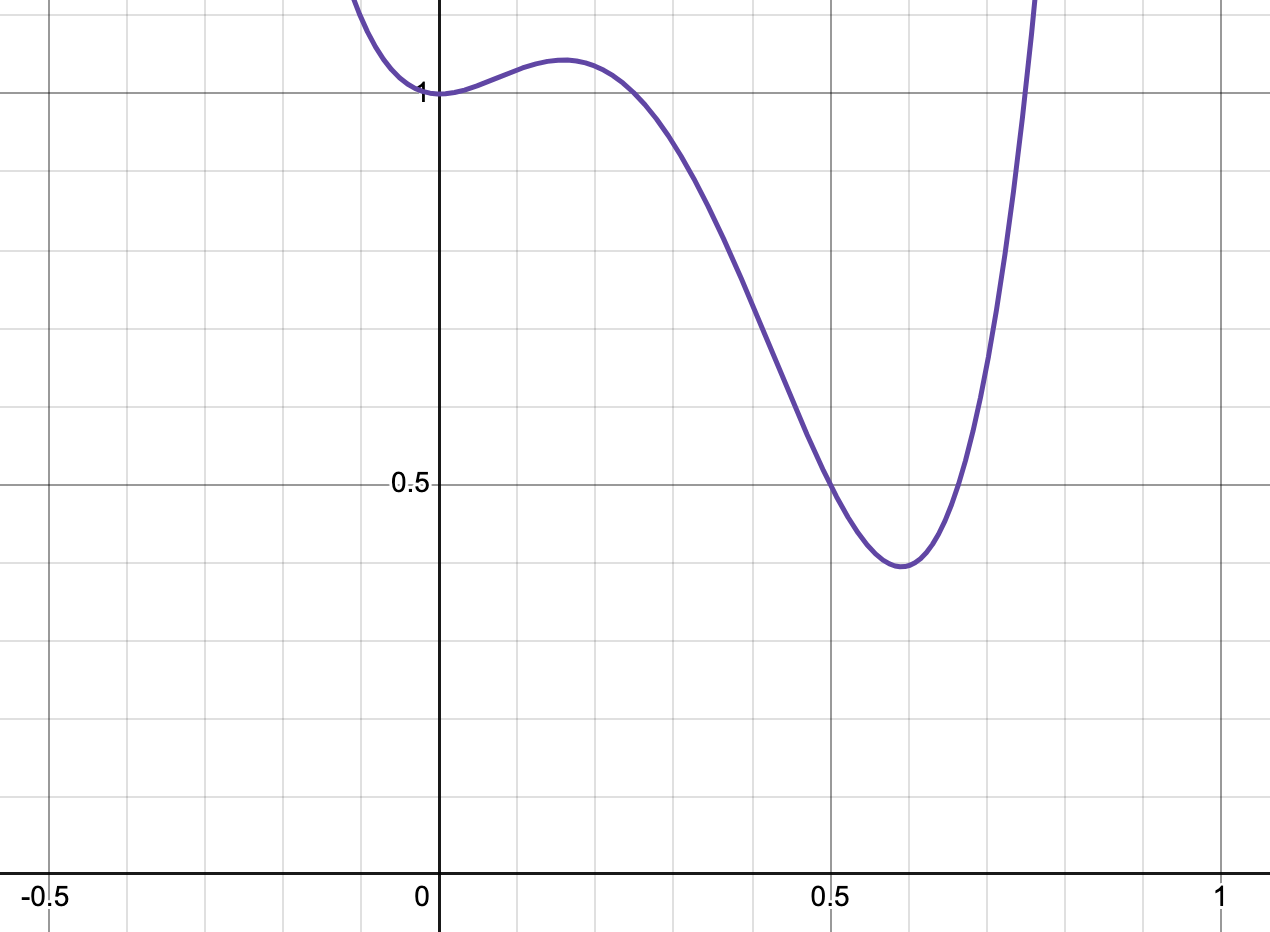
\includegraphics[width=0.4\textwidth]{fig41}
	\caption*{$F_t$}
\end{figure}

Em fim, no caso de $\mathbb{R}^{2}$, suponha que $\omega_0$ e $\omega_1$ são duas formas não degeneradas. Sabemos que em qualquer ponto de $\mathbb{R}^{2}$ elas são um múltiplo da outra. Portanto, uma combinação convexa delas não pode ser degenerada porque é da forma
\[\omega_t=(1-t)\omega_0+t\lambda\omega_0=(1-t+\lambda t)\omega_0.\]
\end{proof}

\begin{thing5}{Problem 3}\leavevmode
Let $(V,\Omega)$ be a symplectic vector space (or vector bundle) and let $W\subseteq V$ be a coisotropic subspace (or bundle).
\begin{enumerate}[label=\alph*.]
	\item Let $E$ be a complement of $W^\Omega$ in $W$, i.e., $W=W^\Omega\oplus E$. Show that the restriction of $\Omega$ to $E$ is nondegenerate.
	\item Let $J$ be a $\Omega$-compatible complex structure, with $g$ the associated inner product. Show that $\Omega$ induces an identification of $J(W^\Omega)=W^\perp$ with $(W^\Omega)^*$. Taking $E$ as the orthogonal complement (with respect to $g$) to $W^\Omega$ in $W$ (this means that $W=W^\Omega\oplus E$), show that the identification
		\[V\cong E\oplus (W^\Omega\oplus (W^\Omega)^*),\]
		is an isomorphism of symplectiv vector spaces (bundles)---on the right-hand-side, $E$ is equipped with its induced symplectic form (see a. above) and $W^\Omega\oplus (W^\Omega)^*$  with its canonical symplectic form.
\end{enumerate}
\end{thing5}

\begin{proof}[Solução]\leavevmode 
\begin{enumerate}[label=\alph*.]
	\item 	Basta ver que $\ker \Omega|_{E}=0$. Se $e\in\ker \Omega|_{E}$, então eu gostaria de ver que $e\in W^\Omega$ para concluir que $e=0$. Seja $w\in W$. Então $\Omega(e,w)=\Omega(e,w_1+w_2)$ com $w_1\in W^\Omega$ e $w_2\in E$. Daí $\Omega(e,w)=0$ já que tanto $\Omega(e,w_1)=0$ porque $e\in E\subset W$ quanto $\Omega(e,w_2)=0$ porque $w_2\in E$.

	\item Considere o mapa
		\begin{align*}
			J(W^\Omega) &\longrightarrow (W^\Omega)^* \\
			Jw &\longmapsto i_w\Omega= \Omega(w,\cdot )
		\end{align*}
		Note que $J(W^\Omega)$ e $W^\Omega$ são espaços vetorias de dimensões iguais, e que esse mapa tem kernel trivial pela não degeneração de $\Omega$. Isso explica que é um isomorfismo.

	Para construir o isomorfismo requerido note que por definição $W\cong E\oplus W^\Omega$. E como mostramos que $W^\perp\cong (W^\Omega)^*$, sabemos que $V\cong W\oplus (W^\Omega)^*$. Daí o isomorfismo algébrico está comprovado por causa de que a soma direita é associativa. Issto é, temos um isomorfismo de espaços vetoriais
	\begin{align*}
		\Phi: V &\longrightarrow E\oplus W^\Omega\oplus (W^\Omega)^* \\
		v &\longmapsto (v_1,v_2,v_3)
	\end{align*}
	onde $g(v_1,v_2)=0$ e $g(v_1+v_2,v_3)=0$.

	Agora vamos comprovar que esse mapa é um simplectomorfismo, 
	
\end{enumerate}
\end{proof}

\paragraph{Problem 4}Prove the following generalizaion of Weinstein's lagrangian neighbourhood theorem to coisotropic submanifolds (due to Gotay, 1982): Let $(M_0,\omega_0)$ be and $(M_1,\omega_1)$ be symplectic manifolds, and $\iota_0:Q\longrightarrow M_0$, $\iota_1:Q\longrightarrow M_1$ be coisotropic embeddings. If $\iota^*_0\omega_0=\iota_1^*\omega_1$ then there exist open  neighbourhoods $\mathcal{U}_0$ and $\mathcal{U}_1$ of $Q$, in $M_0$ and $M_1$, and a diffeomorphism $\varphi:\mathcal{U}_0\longrightarrow \mathcal{U}_1$ such that $\varphi(p)=p$ for all $p\in Q$ and $\varphi^*\omega_1=\omega_0$.

\begin{proof}[Solução]\leavevmode
	Estamos aqui:
	\[\begin{tikzcd}
		(M_0,\omega_0)&&(M_1,\omega_1)\\
	&Q\arrow[ul,"\iota_0",hook]\arrow[ur,"\iota_1",hook,swap]
	\end{tikzcd}\]
Em aula demostramos que:
\begin{thm}[Teorema de Darboux generalizado Vers\~ao 2.0]\leavevmode
	Suponha que, além do diagrama anterior, temos um isomorfismo de fibrados simpl\'ecticos
	\[\begin{tikzcd}
	TM_0|_{Q}\arrow[rr,"\phi"]\arrow[dr,swap]&&TM_1|_{Q}\arrow[dl]\\
	&Q
	\end{tikzcd}\]
	tal que $\phi|_{TQ}:TQ\to TQ$ é $\operatorname{id}_{TQ}$.

	Ent\~ao $\phi$ estende a derivada de um simplectomorfismo
	\[\begin{tikzcd}
	U_0\subset M_0\arrow[rr,"\varphi"]&&U_1\subset M_1\\
	&Q\arrow[ul]\arrow[ur,swap]
	\end{tikzcd}\]
	i.e.,
	\[d\varphi|_{Q}=\phi:TM_0|_{Q}\to TM_1|_{Q}\]
	Em palavras: a derivada do simplectomofismo (entre as vizinhanças de $M_1$ e $M_2$) que obtemos é estendida pelo isomorfismo simpl\'etico dos fibrados tangentes que nos foi dado.
\end{thm}
Portanto, para nosso exercício só precisamos achar um simplectomorfismo $\phi$ de fibrados tangentes que restringe a identidade no $TQ$.

Também é bom lembrar que na prova do teorema das vizinhanças lagrangianas construiimos esse simplectomorfismo de fibrados do seguinte jeito:
	\[\begin{tikzcd}
	&T\mathcal{L}\oplus (T\mathcal{L})^*\arrow[dr,"\cong "]\\
	TM|_{\mathcal{L}}\arrow[rr,"\phi"]\arrow[ur,"\cong "]&&T(T^*\mathcal{L})|_{\mathcal{L}}
	\end{tikzcd}\]
	Issto é, mostrando que, no caso lagragiano, existe um isomorfismo de fibrados tangentes entre o fibrado tangente da variedade ambiente restrito à subvariedade lagrangiana e a soma direita $T\mathcal{L}\oplus (T\mathcal{L})^*$. Aplicando isso usando como variedade ambiente tanto $M$ quanto $T^*M$ construimos o diagrama anterior.

	A estrutura complexa foi usada para obter a descomposição $T\mathcal{L}\oplus (T\mathcal{L})^*$: o que fizemos foi construir o complemento ortogonal usando a métrica compatível e daí mostramos que esse complemento é de fato isomorfo a $(T\mathcal{L})^*$.

	No caso coisotrópico temos, pelo exercício anterior, dois isomorfismos de fibrados
\begin{align*}TM_1\cong E_1\oplus \Big(TQ^\omega\oplus (TQ^\omega)^*\Big),\qquad \qquad 
TM_2&\cong E_2\oplus \Big(TQ^\omega\oplus (TQ^\omega)^*\Big)
\end{align*}
então é claro que se $E_1\cong E_2$ terminhamos. Mas $E_i$ é só o complemento ortogonal de $TQ^\omega$ respeito à métrica compatível $g_i$ em $TQ$, enquanto $g_1$ e $g_2$ coincidem em $TQ$ já que $\omega_1|_{Q}=\omega_2|_{Q}$ por hipótese (o pullback das incluções coincide). Note que também é imediato que a restrição desse isomorfismo a $TQ$  é a identidade.
\end{proof}
\clearpage
\begin{minipage}{\textwidth}
	\begin{minipage}{1\textwidth}
		Geometria Simpl\'etica \hfill Daniel González Casanova Azuela
		
		{\small Profs. Henrique Bursztyn e Leonardo Macarini\hfill\href{https://github.com/danimalabares/sg}{github.com/danimalabares/sg}}
	\end{minipage}
\end{minipage}\vspace{.2cm}\hrule

\vspace{10pt}
\section{Lista 5}

\begin{thing1}{Problem 1}\leavevmode
	Let  $G$ be a Lie group. Let $X:G\longrightarrow TG$ be a section of the projection $TG\longrightarrow G$, not necessarily smooth. Show that if  $X$ is left invariant (i.e., $dL_g(X)=X\circ L_g$ for all $g\in G$), then $X$ is automatically smooth.

	Conclude that an analogous result holds for differential forms: if a section $\eta:G\to \Lambda^{k}(T^*G)$ is left-invariant ($L^*_g\eta=\eta$), then $\eta$ is a smooth $k$-form. Check that an analogous result holds for $G$-invariant forms on a homogeneous manifold.
\end{thing1}

\begin{proof}[Solution]\leavevmode
	We know that $X_g=dL_g(X_e)$. We want to show that the map $G \to TG:g\mapsto dL_g(X_e)$ is smooth. Suggestion by \href{https://math.stackexchange.com/questions/1126553/left-invariant-vector-fields-smoothness}{Ted Shiffrin at StackExchange} is to consider 
	\begin{align*}
		\mu: G\times G &\longrightarrow G \\
		(g,h) &\longmapsto L_gh=gh
	\end{align*}
	which is smooth and thus has smooth differential which \href{https://math.stackexchange.com/questions/1740179/differential-of-the-multiplication-and-inverse-maps-on-a-lie-group}{turns out to have the expression}
	\begin{align*}
		d\mu: TG\times TG &\longrightarrow TG \\
		(u_g,v_h) &\longmapsto dR_hu_g+dL_g v_h
	\end{align*}
	Choosing $g$ arbitrary, $h=e$, $u_g=0$ and $v_h=X_e$, we obtain
	\[d\mu(u_g,v_h)=dL_gX_e\]
	and, as we have said, this differential depends smoothly on $g$.

	The pullback map is an induced map by $L_g$ on the Grassman algebra:
	\begin{align*}
		L_g^*: \Lambda^{k}(G) &\longrightarrow \Lambda^{k}(G) \\
		\eta &\longmapsto \begin{aligned}
			L_g^*\eta: \mathfrak{X}^k(G) &\longrightarrow \mathbb{R} \\
			(X_1,\ldots,X_k) &\longmapsto \eta(dL_gX_1,\ldots,dL_gX_1)
		\end{aligned}
	\end{align*}
and we have by hypothesis that 
\[L_g^*\eta=\eta.\]

Similarly, group multiplication $\mu$ induces a map on the Grassman algebra:
\begin{align*}
	\mu: \Lambda^{k}(G) \times \Lambda^{k}(G)&\longrightarrow \Lambda^{k}(G) \\
	(\alpha,\beta) &\longmapsto R_h^*\alpha+L_g^*\beta
\end{align*}
so again chosing $\alpha=0$ and $\beta=\eta$ we see that $\eta$ is smooth.

Now let $\eta$ be a $G$-invariant form on a homogeneous manifold $X$. Following \href{https://math.stackexchange.com/questions/4298636/smoothness-of-a-g-invariant-k-form}{Jack Lee's suggestion}, we can pull back $\eta$ to $G$ via the map $\pi:G\to X$, $g\mapsto g\cdot p$ for any fixed $p \in X$. This gives a form $\pi^*\eta$ on $G$ that is left-invariant since  $\eta$ is $G$-invariant: pushing vectors with left-multiplication preserves the orbit of a given point. More explicitly:
\begin{align*}
	L^*_g(\pi^*\eta)&=\pi^*\eta\qquad \text{because}\qquad 
	L^*_g(\pi^*\eta)=\eta\circ d\pi\circ dL_g
\end{align*}
and $\eta$ is constant along vectors on the orbit of $p$, which are the images of $d\pi\circ dL_g$. By the previous exercise we see that $\pi^*\eta$ is smooth.

Then we notice that $\pi$ is a submersion. This follows since $\pi$ is a surjective map (bacuse $X$ is homogeneous)  of constant rank. Constant rank means that $d\pi$ has the same rank at every point of $G$. This can be seen moving around the tangent spaces of both  $G$ and $X$ using the differentials of both the action of  $G$ on $M$, and the left-translation action of $G$ on $G$ as follows. There is a commutative diagram:
\[\begin{tikzcd}
	T_gG\arrow[r,"d\pi"]\arrow[d,swap,"d(\text{action}) "]&T_{gp}X\arrow[d,"d(\text{action})" ]\\
	T_{hg}G\arrow[r,"d\pi"]&T_{hgp}X
\end{tikzcd}\]
and those vertical differentials are diffeomorphisms by smothness of the actions.

Finally we conclude by taking a local inverse $\sigma$ of $\pi$ via inverse function theorem. Then we simply notice that $\eta=\sigma ^*\pi^*\eta$, which is smooth by construction.
\end{proof}

\begin{thing4}{Problem 2}\leavevmode
	\begin{enumerate}[label=\alph*.]
		\item Prove that any connected Lie group $G$ is generated as a group by any open neighbourhood $U$ of the identity element (i.e. $G=\bigcup_{n=1}^\infty U^n$).
		\item Suppose that two Lie group homomorphisms $\varphi,\psi:G\to H$ are such that $d\varphi|_{e}=d\psi|_{e}$. Show that $\varphi$ and $\psi$ coincide on the connected component of $G$ containing the identity $e$.
	\end{enumerate}
\end{thing4}

\begin{proof}[Solution]\leavevmode
	\begin{enumerate}[label=\alph*.]
		\item Let $U$ be an open  neighbourhood of the identity and define
			\[U^n:=\{g_1\cdot\ldots \cdot g_n:g_{i}\in U\}\]
		for $n \in\mathbb{N}\setminus\{0\}$. We will show that $\bigcup_{n \in\mathbb{N}} U^n$ is a (non-empty, which is trivial since it contains the identity) closed and open set, implying it is $G$ by connectedness.

		We know that for every $g\in G$ right-multiplication $L_g$  is a diffeomorphism of $G$ (because its inverse is $L_{g^{-1}}$). So it is an open map. This means that $U\cdot g$ is open. Now
		\[U^2=U\cdot U=\bigcup_{g\in U}U\cdot g \]
		must be open. Likeways $U^n$ is open and so is $\bigcup_{n \in\mathbb{N}} U^n$.

		To see that $\bigcup_{n \in\mathbb{N}} U^n$ is also closed, notice that any open subgroup of a topological group is also closed. To see this in our case call $H:=\bigcup_{n \in\mathbb{N}} U^n$. We'll show that $G\setminus H$ is open. Take $g \in G\setminus H$, the set $g\cdot H$ is in fact an open neighbourhood of $g$ contained in $G\setminus H$. Indeed, if $h\in g\cdot H\cap H$, then we can take the inverse $h^{-1}\in H$ and we get that $h^{-1}hg=g\in H$ but that's not possible.



		\item Let $g\in G$ be any element. Suppose we find a vector $v\in T_eG$ such that its integral curve $\gamma$ passes through $g$ at time $t_0$. Then we can map this vector both by $d\varphi$ and $d\psi$ to obtain a vector $w:=d_e\varphi(v)=d_e\psi(v)\in T_eH$. Then the integral curve of  $w$ is the same as the integral curve of $v$ pushed by either of  $\varphi$ or $\psi$ because both are solutions to the same differential equation.

			Then we get that
			\[\gamma(t_0)=g\implies \varphi(g)=\varphi(\gamma(t_0))=\psi(\gamma(t_0))=\psi(g)\]
$\mathsf{OK}$ now we only need to find the vector $v$. The statement is that for every $g$ in the connected component of the identity there is a maximal integral curve starting at the identity passing through $g$. Since $g$ is the same connected component as the identity we can find a curve connecting them. But this curve need not be a maximal integral curve nor homotopic to one. {\color{3}I couldn't find such a vector!} 

	\end{enumerate}
\end{proof}

\begin{thing1}{Problem 3}\leavevmode
	Consider the Lie groups $\mathsf{SU}(2) =\{A\in\mathcal{M}_{2}(\mathbb{C})|AA^*=\operatorname{Id}, \det A=1\}$ and $\mathsf{SO}(3) =\{A\in\mathcal{M}_{3}(\mathbb{R})|AA^{\mathbf{T}}=\operatorname{Id},\det A=1\}$.
	\begin{enumerate}[label=\alph*.]
		\item Show that
		\[\mathsf{SU}(2) =\left\{ \begin{pmatrix} a&b\\-\bar{b}&\bar{a} \end{pmatrix} ,a,b\in\mathbb{C},|a|^2+|b|^2=1\right\} \]
		Conclude that, as a manifold $\mathsf{SU}(2)$ is diffeomorphic to $S^3$ (hence it is simply connected).

		Recall the definition of the quaternions $\mathbb{H}$. Show that the sphere $S^3$, seen as quaternions of norm 1, inherits a Lie group structure with respect to which it is isomorphic to $\mathsf{SU}(2)$.

	\item Verify that
		\begin{equation}\label{eq:1}
			\mathfrak{su}(2) =\left\{ \begin{pmatrix} i\alpha &\beta\\-\bar{\beta} &-i\alpha \end{pmatrix} ,\alpha\in\mathbb{R},\beta\in\mathbb{C} \right\} .
		\end{equation}
		Consider the identification $\mathfrak{su}(2) \cong \mathbb{R}^{3}$, that takes the element in $\mathfrak{su}(2)$ determined by $\alpha,\beta$ to the vector $(\alpha,\operatorname{Re}\beta,\operatorname{Im}\beta)$ in $\mathbb{R}^{3}$. Observe that, with respect to this identification, $ \det $ in $\mathfrak{su}(2)$ corresponds to $\|\cdot\|^2$ in $\mathbb{R}^{3}$.


	\item Verify that each element $A\in\mathsf{SU}(2)$ defines a linear transformation on the vector space $\mathfrak{su}(2)$ by conjugation: $B\mapsto ABA^{-1}$. Show that, with the identification $\mathfrak{su}(2) \cong \mathbb{R}^{3}$, we obtain a representation (i.e., a linear action) of $\mathsf{SU}(2)$ on $\mathbb{R}^{3}$ that is norm preserving. Conclude that we have homomorphism $\phi:\mathsf{SU}(2) \to \mathsf{O}(3)$, verifying that is image is $\mathsf{SO}(3)$ and its kernel is $\{\operatorname{Id},-\operatorname{Id}\}$.

	\item Conclude that $\mathsf{SU}(2) \cong S^3$ is a double cover of $\mathsf{SO}(3)$ *hence is its universal cover, since it's simply connected), qnd the covering map identifies antipodal points of $S^3$. Hence, as manifolds, $\mathsf{SO}(3)$ is identified with $\mathbb{R}P^{3}$.
	\end{enumerate}
\end{thing1}

\begin{proof}[Solution]\leavevmode
	\begin{enumerate}[label=\alph*.]
		\item It is very easy to see that a matrix 
			\[A:=\begin{pmatrix} a &b\\c & d \end{pmatrix} \in\operatorname{Mat}_{2}(\mathbb{C})\]
			satisfying $A A^*=\operatorname{Id}\iff A^*=A^{-1}$ must be of the form
			\[\begin{pmatrix} a &b\\-\bar{b}&\bar{a} \end{pmatrix} \]
			since $A^*=A^{-1}$ translates to
			\[\begin{pmatrix} \bar{a} &\bar{c}\\\bar{b}&\bar{d} \end{pmatrix} =\begin{pmatrix} d&-b\\-c&a\end{pmatrix} \]
			which yields immediately $\bar{a} =d$ and $c=-\bar{b}$.

			Conversely, if $|a|^2+|b|^2=1$ the matrix \[B:=\begin{pmatrix} a &b\\-\bar{b}&\bar{a} \end{pmatrix}\] has determinant
			 \[\det B=a\bar{a}+b \bar{b}=|a|^2+|b|^2=1 \]
			 and its inverse is
			 \[B^{-1}=\begin{pmatrix} \bar{a}&-b\\\bar{b}&a \end{pmatrix} =B^*.\]


			Having estabilshed this expression for $\mathsf{SU}(2)$, it is clear that it is diffeomorphic to $S^3$ since its parameters $a,b\in\mathbb{C}$, $|a|^2+|b|^2=1$, can be understood as vectors $x\in\mathbb{R}^{4}$ of norm 1.

		The quaternions are the only 4-dimensional real division algebra. This means it is a 4-dimensional real vector space equipped with a (non-commutative) multiplication. They are also equipped with a norm that coincides with euclidean norm. With respect to this norm we define the unit sphere $S^3$. 
		
			To see that $S^3$ is a Lie subgroup we first need to check that it is closed under quaternion product. The easiest way to see that is via quaternion conjugate: if $x=x_1+ix_2+jx_3+kx_4$ is a quaternion, its conjugate is $\bar{x}=x_1-ix_2-jx_3-kx_4$. It may be computed that the norm is given by $|x| =x\bar{x}$. Then we see that if $x,y\in S^3$
			\[|xy\overline{xy}|=|xy\bar{y}\bar{x}| =\Big|x|y| \bar{x}\Big|=1\]
			Then the fact that $S^3$ is a Lie group follows from the fact that the restricition (the multiplication and inverse map) of smooth maps to embedded submanifolds remains smooth.

			An identification between $S^3\subset \mathbb{H}$ and $\mathsf{SU}(2)$ as expressed above is given by
			\[a+bi+cj+dk\longmapsto \begin{pmatrix} a+bi&c+di\\-c+di&a-bi\end{pmatrix} \]
			Checking that this map is a group isomorphism ammounts to checking that matrix multiplication in $\mathsf{SU}(2)$ is the same as quaternion multiplication.


			\item (Proof from \cite{hall}, prop. 3.24.) We will show that $\mathfrak{su}(2)$ is the space of traceless anti-hermitian matrices and \cref{eq:1} will follow.
				\begin{enumerate}[label=\textbf{Step \arabic*}]
					\item Show that the Lie algebra of a matrix Lie group $G$, defined as the tangent space at identity, is the same as the matrices $X$ such that $ \operatorname{exp}(tX) \in G$ for all $t\in\mathbb{R}$. (Inspired, though the proof is different because his definitions are different, in \cite{hall}, coro. 3.46.)

						\begin{proof}[Proof of Step 1]\leavevmode
							First suppose that $X$ is such that $\operatorname{exp}(tX)\in G$ for all $t\in\mathbb{R}$. Then the curve $\gamma(t)=\operatorname{exp}(tX)$, which is contained in $G$, passes through the identity at $t=0$ with velocity $X$, meaning that $X$ is in the tangent space of the identity element.

							For the converse suppose that $X \in T_{\operatorname{Id}}G$. Our definition of exponential map is to move along the integral curve of $X$, say $\gamma_X$, by 1 unit of time. Then
							\[\operatorname{exp}(tX) =\gamma_{tX}(1)=\gamma_X(t)\in G\]
							by homogenity property.

							%Define a curve $\gamma$ via the exponential map (seen in lectures, also see figure): $\gamma(t)=\operatorname{exp}(tX)$ which is in $G$ by definition of exponential map.
	\begin{figure}[H]		\centering
		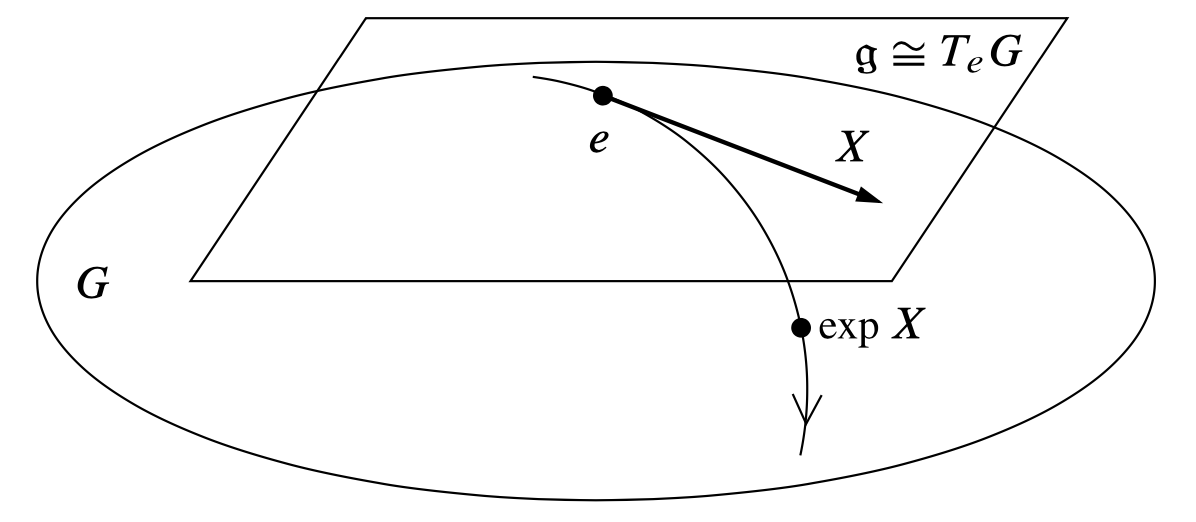
\includegraphics[width=0.4\textwidth]{fig2}	
	\end{figure}
						\end{proof}

					\item Then we look for the matrices such that for all $t\in\mathbb{R}$,
						\[\operatorname{exp}(tX)^* =\operatorname{exp}(tX)^{-1}=\operatorname{exp}(-tX) \qquad \text{ and} \qquad \det \operatorname{exp}(tX)=1. \]
						This means that
						\[\operatorname{exp}(tX^*) =\operatorname{exp}(-tX) \qquad \text{and} \qquad \operatorname{ Tr}(X)=0.\]
						The first implication is the result of the general facts that $(e^{A})^*=e^{A^*}$ and $(e^A)^{-1}=e^{A^{-1}}$. Let's have a look at the second one:
\begin{quotation}
	{\color{3}$(e^A)^{-1}=e^{A^{-1}}$}\hspace{.5em}This is nicely shown in \cite{lee} as follows. For any $X\in\mathsf{Lie}(G)$ map $t\mapsto \operatorname{exp}(tX)$ is a group homomorphism  $\mathbb{R}\to G$ because $\operatorname{exp}((t_1+t_2)X)=\operatorname{exp}(t_1X)\operatorname{exp}(t_2X)$ (but of course that should be justified…) and from this it follows that this map preserves inverses, which what we wanted.
\end{quotation}

						Now let's have a look at why determinant 1 in Lie group translates to vanishing trace in Lie algebra.
\begin{quotation}
	{\color{3}\bfseries $\forall X\in\mathcal{M}_{n}(\mathbb{C}), \;\det e^X=e^{\operatorname{tr}X}$.}\hspace{.5em}This is easy to see if $X$ is diagonalizable with eigenvalues  $\lambda_1,\ldots,\lambda_n$; then the eigenvalues of $e^{X}$ are $e^{\lambda_1},\ldots,e^{\lambda_n}$. So $\det e^X=\prod e^{\lambda_i}=e^{\sum \lambda_i}=e^{\operatorname{tr}X}$. But if $X$ is not diagonalizable we must do Jordan decomposition and some more computations.
\end{quotation}

						Finally, differentiating and evaluating at $t=0$ the equation $\operatorname{exp}(tX^*) =\operatorname{exp}(-tX)$ gives $X^*=-X$. (See \cite{hall}, prop. 2.4. It is intuitive but not immediate.)

						In conclusion, we see that
						\[\mathfrak{su}(2)=\{X\in\mathcal{M}_{2\times 2}(\mathbb{C}):X^* =-X\text{ and }\operatorname{Tr}(X)=0 \}\]
		
					\item It is immediate that the right-hand side in \cref{eq:1} is contained in the set above. For the other inclusion first notice that the condition $X^*=-X$ makes the entries in the diagonal be such that
						\begin{align*}							x+iy&=-\overline{x+iy}=-(x-iy)=-x+iy\implies x=-x\implies x=0						\end{align*}
						while the traceless condition implies the two entries in the diagonal must be additive inverses. For the entries in the antidiagonal we literally see the definition of conjugate transpose.
				\end{enumerate}

Now let's identify $\mathfrak{su}(2)$ with $\mathbb{R}^{3}$ via $\alpha,\beta \mapsto (\alpha,\operatorname{Re}\beta,\operatorname{Im}\beta)$. We immediately see that
\[\det \begin{pmatrix} i\alpha&\beta\\-\bar{\beta} &-i\alpha\end{pmatrix} =i\alpha(-i\alpha)=\beta(-\bar{\beta} )=\alpha^2+|\beta|^2=\|(\alpha,\operatorname{Re}\beta,\operatorname{Im}\beta)\|^2\]

\item De acordo com o exercício anterior, é suficiente mostrar que $ABA^{-1}$ tem traço zero e $ABA^{-1}=-(ABA^{-1})^*$. A primeira propriedade é imediata dado que, em geral, $\operatorname{Tr}(XY)=\operatorname{Tr}(YX)$. Para a segunda propriedade note que
	\[(ABA^{-1})^*=(A^{-1})^*B^*A^*=(A^*)^*(-B)A^{-1}=-ABA^{-1}\]
	O fato de que essa ação em $\mathsf{SU}(2)$ preserva a norma é immediato do item anterior e do fato de que determinante de um produto de matrizes é o produto dos determinantes.

	Isso significa que cada elemento em $\mathsf{SU}(2)$ age como uma isometria linear $\mathbb{R}^{3}\to \mathbb{R}^{3}$, i.e. temos um mapa 
	\begin{align*}
	\varphi:\mathsf{SU}(2) &\longrightarrow \mathsf{O}(3) \\
	A &\longmapsto I_A
\end{align*}
onde
\begin{align*}
	I_A: \mathfrak{su}(2) \cong \mathbb{R}^{3} &\longrightarrow \mathfrak{su}(2) \cong \mathbb{R}^{3} \\
		B &\longmapsto ABA^{-1}
\end{align*}

	$\varphi$ é um homomorfismo já que para $A,A'\in  \mathsf{SU}(2)$ e $B\in\mathfrak{su}(2)$ temos que
	\[I_{A A'}B=(A A')B(A A')^{-1}=A\Big(A'B(A')^{-1}\Big)A^{-1}=(I_A \circ  I_{A'})B.\]
	Para determinar que matriz corresponde com a transformação $I_A$ mediante a identificação $\mathfrak{su}(2) \cong \mathbb{R}^{3}$, suponha que
	\[A=\begin{pmatrix} a&b\\-\bar{b}&\bar{a} \end{pmatrix}, \qquad B=\begin{pmatrix} i\alpha &\beta\\-\overline{\beta} &-i\alpha\end{pmatrix}  \]
	Daí,
\begin{align*}
	ABA^{-1}&=ABA^*=\begin{pmatrix} a&b\\-\bar{b}&\bar{a} \end{pmatrix}\begin{pmatrix} i\alpha &\beta\\-\overline{\beta}&-i\alpha \end{pmatrix}\begin{pmatrix} \overline{a}&-b\\\bar{b}&a \end{pmatrix} \\
&=\begin{pmatrix} a&b\\-\bar{b}&\bar{a} \end{pmatrix}\begin{pmatrix} i \alpha\overline{a}+\beta\overline{b} & -i\alpha b + \beta a\\ -\overline{\beta}\overline{a}-i\alpha \overline{b} & \overline{\beta}b-i \alpha a \end{pmatrix}\\
&=\begin{pmatrix} a(i \alpha \overline{a}+\beta\overline{b})+b(-\overline{\beta}\overline{a}-i\alpha\overline{b}) &  a(-i \alpha b+\beta a)+b(\overline{\beta}b-i\alpha a)\\ * & * \end{pmatrix} 
\end{align*}
Daí, se $(x_1,x_2,x_3)$ é vetor correspondente a $ABA^{-1}$, vemos que
\begin{align*}
	ix_1&=a(i \alpha \overline{a}+\beta\overline{b})+b(-\overline{\beta}\overline{a}-i\alpha\overline{b}) \\
	&=i|a|^2\alpha+a\overline{b}\beta-b\overline{a}\overline{\beta}-i\alpha|b|^2\\
	x_2+ix_3&=a(-i \alpha b+\beta a)+b(\overline{\beta}b-i\alpha a)\\
	&=-iab \alpha
\end{align*}
Agora considere a base de $\mathfrak{su}(2)$ dada por
\[\begin{pmatrix} i&0\\0&-i \end{pmatrix},\quad \begin{pmatrix} 0&1\\-1&0 \end{pmatrix} ,\quad \begin{pmatrix} 0&i\\-i&0 \end{pmatrix}  \]
que corresponde à base canônica de $\mathbb{R}^{3}$. A matriz da transformação $I_A$  terá nas columnas os vetores correspondentes às imagens dessas treis matrizes. Usando as fórmulas anteriores, concluimos que
\[I_A=\begin{pmatrix} |a|^2-|b|^2 & \operatorname{Re}(-i(a\overline{b}-b \overline{a}))& \operatorname{Re}(a \overline{b}+b \overline{a})\\
0 & \operatorname{Re}(a^2+b^2)& \operatorname{Re}(i(a^2-b^2)) \\
-2ab& \operatorname{Im}(a^2+b^2)&\operatorname{Im}(i(a^2-b^2))\end{pmatrix} \]
\end{enumerate}
Para calcular o kernel de $\varphi$ suponha que a matriz anterior é a identidade. Segue que
\begin{align*}
	\ddot{\cap}
\end{align*}

\item Supondo que mostramos que a imagem de $\varphi$ é $\mathsf{SO}(3)$ com kernel $\{\operatorname{Id},-\operatorname{Id}\}$, temos o isomorfismo
	\[\dfrac{\mathsf{SU}(2)}{\{\operatorname{Id},-\operatorname{Id}\}}\cong \mathsf{SO}(3)\]
Suponha que dois elementos $A,B \in\mathsf{SU}(2)$ estão na mesma classe de equivâlencia no quociente. Então
\[AB^{-1}\in\{\operatorname{Id},-\operatorname{Id}\}\iff A=B \text{ ou }A=-B \]
Assim, cada elemento de $\mathsf{SO}(3)$ correponde com dois elementos de $\mathsf{SU}(2)$. Como $\{\operatorname{Id},-\operatorname{Id}\}$ age de maneira prórpia, livre e disonctínua em $\mathsf{SU}(2)$, temos um recobrimento de $\mathsf{SO}(3)$. Também é claro que estamos identificando pontos antípodas de $S^3$ já que ser antípoda em $S^3$ corresponde com o produto com $-\operatorname{Id}$. Note que $\mathbb{R}P^{3}\cong S^3/\mathbb{Z}_2$, de modo que $\mathsf{SU}(2)$ é um recobrimento de $\mathsf{SO}(3)$: cada ponto de $\mathsf{SO}(3)$ tem uma preimagem composta por dois elementos
\end{proof}

\begin{thing4}{Problem 4}\leavevmode
	Let $\mathfrak{g}$ be the Lie algebra of a Lie group $G$, and let  $k:\mathfrak{g} \times \mathfrak{g}\to \mathbb{R}$be a symmetric bilinear form that is $\operatorname{Ad}$-invariant (i.e. $k(\operatorname{Ad}_g(u),\operatorname{Ad}_g(v))=k(u,v)$ for $g\in G$).
	\begin{enumerate}[label=\alph*.]
		\item Show that the map
			\begin{equation}\label{Eq:4a}\begin{aligned}
				k^\sharp:\mathfrak{g}  &\longrightarrow \mathfrak{g}^* \\
				k^\sharp(u)(v) &=k(u,v)\end{aligned}
			\end{equation}
			is $G$-equivariant:
			\[k^\sharp \circ \operatorname{Ad}_g=(\operatorname{Ad}^*)_g\circ k^\sharp,\qquad \forall g\in G\]
			[\textit{Recall:} $(\operatorname{Ad}^* )_g:=(\operatorname{Ad}_{g^{-1}})^*$.] In particular, when $k$ is nondegenerate (i.e. $k^\sharp$ is an isomorphism), the adjoint and coadjoint actions are equivalent.

		\item Verify that \cref{Eq:4a} implies that $k([w,u],v)=-k(u,[w,v])$,  $\forall u,v,w\in\mathfrak{g}$, and that both conditions are equivalent when $G$ is connected.
	\end{enumerate}
\end{thing4}

\begin{proof}[Solução]
	\begin{enumerate}[label=\alph*.]
		\item É só abrir as definições . Fixe um elemento $x\in\mathfrak{g}$. No lado esquerdo, temos
			\[\Big(k^\sharp \circ \operatorname{Ad}_g\Big)(x)=k^\sharp(\operatorname{Ad}_gx)=k(\operatorname{Ad}_gx,\cdot )\]
			e no lado direito,
			\[\Big((\operatorname{Ad}^* )_g\circ k^\sharp \Big) (x)=\operatorname{Ad}^*_g(k^\sharp (x))=\operatorname{Ad}^* _g(k(x,\cdot ))=k(x,\operatorname{Ad}_{g^{-1}}\cdot )\]
			mas, como $k$ é $\operatorname{Ad}$-invariante,
			$k(x,\operatorname{Ad}_{g^{-1}}\cdot )=k(\operatorname{Ad}_gx,\cdot )$.

		\item Must check this later…
	\end{enumerate}
\end{proof}

\begin{thing1}{Problem 5}\leavevmode
For a Lie algebra $\mathfrak{g}$, there is always a canonical bilinear form $k:\mathfrak{g} \times \mathfrak{g} \to \mathbb{R}$, called \textit{\textbf{Killing form}}, given by:
\[k(u,v)=\operatorname{tr}(\operatorname{ad}_u\operatorname{ad}_v).\]
(\textit{Recall:} $\operatorname{ad}_u:\mathfrak{g} \to \mathfrak{g}$, $\operatorname{ad}_u(v)=[u,v]$.)
\begin{enumerate}[label=\alph*.]
	\item Note that $k$ is symmetric, and check that it is  $\operatorname{Ad}$-invariant.
	\item A Lie algebra is called \textit{\textbf{semi-simple}} if $k$ is nondegenerate. Show that $\mathfrak{so}(3)$ is semi-simple.
\end{enumerate}
\end{thing1}

\begin{proof}[Solution]\leavevmode
	\begin{enumerate}[label=\alph*.]
		\item O fato de $k$ ser simétrica segue de que, em geral, $\operatorname{tr}(AB)=\operatorname{tr}(BA)$. Para ver que $k$ é $\operatorname{Ad}$-invariante vamos mostrar que (a idea vem de \href{https://math.stackexchange.com/questions/2409279/showing-killing-form-is-ad-invariant}{StackExchange}):
	\begin{equation}\label{Eq:2}	\operatorname{ad}_{\operatorname{Ad}_gu}=\operatorname{Ad}_g\circ \operatorname{ad}_u\circ \operatorname{Ad}_{g^{-1}}.
		\end{equation}
			Supondo isso, é fácil ver que
			\begin{align*}
				\operatorname{ad}_{\operatorname{Ad}_gu}\circ \operatorname{ad}_{\operatorname{Ad}_{g}v}&=\operatorname{Ad}_{g}\circ \operatorname{ad}_u\circ \operatorname{Ad}_{g^{-1}}\circ \operatorname{Ad}_g\circ \operatorname{ad}_v\circ \operatorname{Ad}_{g^{-1}}\\
				&=\operatorname{Ad}_g\circ \operatorname{ad}_u\circ \operatorname{ad}_v\circ \operatorname{Ad}_{g^{-1}}
			\end{align*}
			e o resultado segue do fato de que a traça é invariante baixo mudanças de coordenadas e que $\operatorname{Ad}_g^{-1}=\operatorname{Ad}_{g^{-1}}$. Isso último segue de que o mapa inverso de $I_g$  é $I_{g^{-1}}$, assim as derivadas deles também são inversa uma da outra.

			Agora vamos mostrar \cref{Eq:2}. Pegue $x\in\mathfrak{g}$. O lado esquerdo diz que
			\[\operatorname{ad}_{\operatorname{Ad}_gu}x=[\operatorname{Ad}_gu,x]\]
			enquanto o direito diz que
			\[\Big(\operatorname{Ad}_g\circ \operatorname{ad}_u\circ \operatorname{Ad}_{g^{-1}}\Big)x=\operatorname{Ad}_g[u,\operatorname{Ad}_{g^{-1}}x]=[\operatorname{Ad}_gu,x\]
			já que $\operatorname{Ad}_g=d_eI_g$ não é apenas um automorfismo linear, mas é um automorfismo de álgebra de Lie, i.e. $\operatorname{Ad}_g[x,y]=[\operatorname{Ad}_gx,\operatorname{Ad}_gy]$ para $x,y\in\mathfrak{g}$. Isso segue do fato de que o pushforward de colchete de Lie de dois campos vetoriais e o colchete dos pushforwards dos campos vetoriais (ver \cite{lee}, coro. 8.31).
		
\item Por enquanto não consegui resolver esse problema:
	\end{enumerate}
\end{proof}

\begin{thing4}{Problem 6}\leavevmode
	Consider the linear isomorphism $\mathbb{R}^{3}\to \mathfrak{so}(3)$, given by
	\[v=(x,y,z)\longmapsto \hat{v}:=\begin{pmatrix} 0&-z&y\\z&0&-x\\-y&x&0 \end{pmatrix} \]
	\begin{enumerate}[label=\alph*.]
		\item Describe the Lie bracket on $\mathbb{R}^{3}$ induced by the commutator in $\mathfrak{so}(3)$, and the inner product in $\mathfrak{so}(3)$ that corresponds to the canonical inner product in $\mathbb{R}^{3}$.

		\item Describe the $\mathsf{SO}(3)$-action on $\mathbb{R}^{3}$ corresponding to the adjoint action, its orbits, as well as its infinitesimal generators. Find (without any calculation!) a description of the coadjoint action on $\mathbb{R}^{3}$ (identified with $(\mathbb{R}^{3})^*$ through the canonical inner product).
	\end{enumerate}
\end{thing4}

\begin{proof}[Solution]\leavevmode
	\begin{enumerate}[label=\alph*.]
		\item Lembre que
			\[\mathsf{SO}(3) =\{A\in\mathcal{M}_{3}(\mathbb{R}):A A^{\mathbf{T}}=\operatorname{Id},\det A=1\}\]
			\[\mathfrak{so}(3) =\{A\in\mathcal{M}_{3}(\mathbb{R}):A=-A^{\mathbf{T}}\}\]
Isso explica por que as matrizes em $\mathfrak{so}(3)$ tem a forma mostrada acima. O isomorfismo com $\mathbb{R}^{3}$ é dado por
	\begin{align*}
		 \mathfrak{so}(3) &\longrightarrow \mathbb{R}^{3} \\
		\begin{pmatrix} 0&-z&y\\z&0&-x\\-y&x&0 \end{pmatrix}  &\longmapsto \begin{pmatrix} x\\y\\z \end{pmatrix} =u\\
		[U,V ]& \longmapsto u\times v\\
		\frac{1}{2}\operatorname{tr}(UV^{\mathbf{T}})&\longmapsto\left<u,v\right> 
	\end{align*}
Para comprovar que de fato o commutador de $\mathfrak{so}(3)$ corresponde com o produto vetorial em $\mathbb{R}^{3}$, considere duas matrizes $U,V\in\mathfrak{so}(3)$ e os vetores correspondentes $u=(u_1,u_2,u_3)$, $v=(v_1,v_2,v_3)$. O commutador é
\begin{align*}
	[U,V]=UV-VU&=\begin{pmatrix} 0&-u_3&u_2\\u_3&0&-u_1\\-u_2&u_1&0 \end{pmatrix} \begin{pmatrix} 0&-v_3&v_2\\v_3&0&-v_1\\-v_2&v_1&0 \end{pmatrix} \\
	&- \begin{pmatrix} 0&-v_3&v_2\\v_3&0&-v_1\\-v_2&v_1&0 \end{pmatrix} 
\begin{pmatrix} 0&-u_3&u_2\\u_3&0&-u_1\\-u_2&u_1&0 \end{pmatrix}\end{align*}
	\end{enumerate}
	a entrada $(3,2)$ da matriz resultante  é a primeira coordenada do vetor correspondente a $[U,V]$; esse numero é claramente $u_1v_3-u_3v_2$. Analogamente, a segunda coordenada é $u_3v_1-u_1v_3$, enquanto a terceira $u_1v_2-u_2v_1$. Essas são as coordenadas de $u\times v$.

Para ver que o produto interno de $\mathbb{R}^{3}$ corresponde com $\frac{1}{2}\operatorname{tr}$ note que
\begin{align*}
	UV^{\mathbf{T}}=U(-V)&=\begin{pmatrix} 0&-u_3&u_2\\u_3&0&-u_1\\-u_2&u_1&0 \end{pmatrix} \begin{pmatrix} 0&v_3&-v_2\\-v_3&0&v_1\\v_2&-v_1&0 \end{pmatrix} \\
		       &=\begin{pmatrix} u_3v_3+u_2v_2&*&*\\ *&u_3v_3+u_1v_1&*\\ *&*&u_2v_2+u_1v_1 \end{pmatrix} 
\end{align*}

\item Agora vamos calcular a ação adjunta. 
Primeiro notemos que a ação adjunta, definida como a derivada do operador $I_A(X)=AXA^{-1}$, é ela mesma. Talvez esse é um fato obvio porque $I_A$  é um mapa linear, e a sua derivada coincide com ele. Porém, tem um argumento mais explícito no \href{https://math.stackexchange.com/questions/512026/prove-that-the-action-of-a-lie-group-on-its-lie-algebra-via-the-adjoint-represen}{StackExchange}: a ação adjunta em um vetor  $X\in\mathfrak{so}(3)$ que seja a derivada em $t=0$ da curva $\gamma\subset \mathsf{SO}(3)$, i.e.  $\gamma'(0)=X$, é simplesmente $\frac{d}{dt}A\gamma(t)A^{-1}\Big|_{t=0}=AXA^{-1}$. A observação chave é que como a álgebra de Lie $\mathfrak{so}(3)$ é um álgebra de matrizes, o produto do lado direito está bem definido.

Agora vamos achar uma matriz que representa esse operador linear quando identificamos $\mathfrak{so}(3)$ com $\mathbb{R}^{3}$. Ou seja, queremos achar uma matriz  $\overline{\operatorname{Ad}_A}$ tal que $\operatorname{Ad}_AX=AXA^{-1}\rightsquigarrow \overline{\operatorname{Ad}_A}x$ onde $x\in\mathbb{R}^{3}$  representa a matriz $X\in\mathfrak{so}(3)$. Vamos ver que de fato essa matriz é $A$.

\begin{align*}AXA^{\mathbf{T}}&=\begin{pmatrix}a_{11}&a_{12}&a_{13}\\ a_{21}&a_{22}&a_{23}\\ a_{31}&a_{32}&a_{33}\end{pmatrix}\begin{pmatrix}0&-z&y\\ z&0&-x\\ -y&x&0\end{pmatrix}\begin{pmatrix}a_{11}&a_{21}&a_{31}\\ a_{12}&a_{22}&a_{32}\\ a_{13}&a_{23}&a_{33}\end{pmatrix}\\
&=\begin{pmatrix}a_{11}&a_{12}&a_{13}\\ a_{21}&a_{22}&a_{23}\\ a_{31}&a_{32}&a_{33}\end{pmatrix}\begin{pmatrix}-za_{12}+ya_{13}&-za_{22}+ya_{23}&-za_{32}+ya_{33}\\ a_{11}z-xa_{13}&za_{21}-xa_{23}&za_{31}-xa_{33}\\ -ya_{11}+xa_{12}&-ya_{21}+xa_{22}&-ya_{31}+xa_{32}\end{pmatrix}\end{align*}
Daí, se o vetor correspondente a $AXA^{\mathbf{T}}$ e $(x',y',z')$, sabemos que suas coordenadas estão nas entradas $(3,2)$, $(1,3)$ e $(2,1)$, respetivamente, da matriz que resulta acima. Ou seja,
\begin{align*}
	x'&=a_{31}(-za_{22}+ya_{23})+a_{32}(za_{21}-xa_{23})+a_{33}(-ya_{21}+xa_{22})\\
	y'&=a_{11}(-za_{32}+ya_{33})+a_{12}(za_{31}-xa_{33})+a_{13}(-ya_{31}+xa_{32})\\
	z'&=a_{21}(-za_{12}+ya_{13})+a_{22}(a_{11}z-xa_{13})+a_{23}(-ya_{11}+xa_{12})
\end{align*}
Para achar a matriz buscada simplesmente calculamos as coordenadas dos vetores canónicos de $\mathbb{R}^{3}$.

\begin{itemize}
\item Se $(x,y,z)=(1,0,0)$ obtemos  \[(x',y',z')=(-a_{23}a_{32}+a_{22}a_{33},-a_{12}a_{33}+a_{13}a_{32},-a_{22}a_{13}+a_{23}a_{12})\]
\item Se $(x,y,z)=(0,1,0)$ obtemos  \[(x',y',z')=(a_{23}a_{31}-a_{21}a_{33},a_{11}a_{33}-a_{13}a_{31},a_{21}a_{13}-a_{23}a_{11})\]
\item Se $(x,y,z)=(0,0,1)$ obtemos  \[(x',y',z')=(-a_{22}a_{31}+a_{21}a_{32},-a_{11}a_{32}+a_{12}a_{31},-a_{21}a_{12}+a_{22}a_{11})\]
\end{itemize}
Esses treis vetores em colunas conformam a matriz que buscamos, que podemos chamar por enquanto $\mathbf{C}$. Para mostrar que $\mathbf{C}=A$ basta ver que $\mathbf{C}A^{\mathbf{T}}=\operatorname{Id}$.

É simples ver que as coordenadas de $\mathbf{C}$ são distintos menores (determinantes de sub-matrizes de $2\times 2$) de $A$. Quando calculamos o produto $\mathbf{C} A^{\mathbf{T}}$, vemos que nas tres entradas da diagonal aparece o determinante de $A$, que é 1. As entradas fora da diagonal devem ser zero. Fazendo contas não achei immediato, mas o resultado é um fato de álgebra linear: a matriz que calculamos se chama \href{https://en.wikipedia.org/wiki/Minor_(linear_algebra)#Cofactor_expansion_of_the_determinant}{\textit{\textbf{matriz de cofactores}}} e satisfaz, em geral,
\[A^{-1}=\frac{1}{\det A}\mathbf{C}^{\mathbf{T}}\]
A menos dessa continha, isso mostra que a ação adjunta de $\mathsf{SO}(3)$ em $\mathbb{R}^{3}$ é por rotações com eixos que passam pela origem. Segue que a órbita da origem é trivial. As órbitas dos outros pontos são quocientes $\mathsf{SO}(3)/S^1$, já que as órbitas são difeomorfas ao quociente do grupo sobre estabilizador (pode pensar que a órbita é uma variedade homogénea). Ademais, $\mathsf{SO}(3)$ age transitivamente em $S^2$ com estabilizador também $S^1$. Segue que as órbitas são $\mathsf{SO}(3)/S^1\overset{\operatorname{dif}}{\simeq} S^2$.

Em geral, o gerador infinitesimal da ação adjunta $\operatorname{Ad}_g$ em $u\in\mathfrak{g}$ é $\operatorname{ad}_u=[u,\cdot]$. No nosso caso, para $u\in\mathfrak{so}(3) \cong \mathbb{R}^{3}$, $\operatorname{ad}_u=[u,\cdot ]\rightsquigarrow u\times \cdot$, i.e., é o campo vetorial que em cada ponto de $\mathbb{R}^{3}$ asoccia o produto vetorial dele com $u$.

Por último, a ação coadjunta em $A\in\mathsf{SO}(3)$ é um operador $\operatorname{Ad}^*_A$ satisfazendo para todo $\xi\in  \mathfrak{so}(3)^* \cong \mathbb{R}^{3}$ e $Y\in \mathfrak{so}(3) \cong \mathbb{R}^{3}$,
\[(\operatorname{Ad}^* _A\xi)Y=\xi(\operatorname{Ad}_{A^{-1}}Y).\]
A identificação de $(\mathbb{R}^3)^*$ com $\mathbb{R}^3$ usando o produto interno canônico significa que associamos $\xi$ com algum vetor $V_\xi$ tal que $\xi(Y)=(V_\xi,Y)$ onde $(\cdot,\cdot)$ é o produto interno euclidiano canônico. Como ainda já sabemos que $\operatorname{Ad}_{A^{-1}}$ age em $\mathbb{R}^{3}$ como multiplicação por $A^{-1}$, vemos que
\begin{align*}
	(\operatorname{Ad}^*_A\xi)Y \leftrightsquigarrow (V_\xi,A^{-1}Y).
\end{align*}
Mas ainda, o vetor $V_\xi$ é simplesmente o vetor de coordenadas $(\xi^1,\xi^2,\xi^3)$ se escrevemos $\xi=\sum \xi^idx^i\in (\mathbb{R}^3)^*$. Para descrever as órbitas só note que a expressão acima está determinada por $A$, de modo que a  órbita coadjunta está em correspondência com a $\mathsf{SO}(3)$-órbita do vetor $V_\xi$, que já sabemos que é uma esfera $S^2$.

\iffalse
\begin{align*}
	(\operatorname{Ad}^*_A\mu)Y&=\mu(A^{-1}YA)
\end{align*}
Passando a $\mathbb{R}^{3}$, podemos usar o produto interno para identificar $\mu$ com o vetor $V_\mu$ tal que $\mu(X)=\left<V_\mu,X\right> $ para todo $X\in \mathbb{R}^{3}\cong \mathfrak{su}(3)$. Lembrando a fórmula que corresponde com o produto interno, obtemos
\begin{align*}
	(\operatorname{Ad}^*_A\mu)Y&=\frac{1}{2}\operatorname{tr}\Big(V_\mu (A^{-1}YA)^{\mathbf{T}}\Big)=\frac{1}{2}\operatorname{tr}(V_\mu A^{\mathbf{T}}YA)
\end{align*}
E isso último é\fi
\end{proof}

\begin{thing1}{Problem 7}\leavevmode
	Let $(V,\Omega)$ be a symplectic vector space, and consider $H:=V\times \mathbb{R}=\{(v,t)\}$. This space $H$ with the multiplication
	\[(v_1,t_1)\cdot(v_2,t_2)=\left( v_1+v_2,\frac{1}{2}\Omega(v_1,v_2)+t_1+t_2 \right) \]
	is a Lie group called the \textit{\textbf{Heisenberg group}} (find the identity elements and inverses in  $H$).
	\begin{enumerate}[label=\alph*.]
		\item Show (directly from the conjugation formula in $H$) that $\operatorname{Ad}_{(v,t)}(X,r)=(X,r+\Omega(v,X))$, for $(X,r)\in\mathfrak{h}=\mathsf{Lie}(H) =V\times \mathbb{R}$. Describe the adjoint orbits, verifying that their possible dimensions are zero and one.
		\item Verify that $\operatorname{ad}_{(Y,s)}(X,r)=(0,\Omega(Y,X))$. [Recalling that $\operatorname{ad}_{(Y,s)}(X,r)=[(Y,s),(X,r)]$, we obtain a formula for the Lie bracket in $ \mathfrak{h}$.]
		\item Describe the coadjoint action of $H$ on $\mathfrak{h}^*=V^*\times \mathbb{R}^*$ and its orbits, analyzing the possible dimensions.
	\end{enumerate}
\end{thing1}

\begin{proof}[Solution]\leavevmode
É imediato que a identidade em $H$ é $(0,0)\in V\times \mathbb{R}$, e o elemento inverso de $(v,t)$  é $(-v,-t)$.
 \begin{enumerate}[label=\alph*.]
	\item Primeiro note que $\operatorname{Ad}_{(v,t)}X=(v,t)\cdot X\cdot(-v,-t)$ onde $\cdot$ denota o produto en $H\cong \mathfrak{h}$ (esse isomorfismo é claro já que $H$ é um espaço vetorial, assim o espaço tangente em $(0,0)$  é isomofo a ele). Para justificar isso (como no exercício anterior), considere uma curva $\gamma\subset H$ tal que $\gamma(0)=(0,0)$ e $\gamma'(0)=(X,r)$. Então 
		\begin{align*}
			\operatorname{Ad}_{(v,t)}(X,r)&=d_{(0,0)}I_{(v,t)}(X,r)=\frac{d}{d\tau}I_{(v,t)}\circ \gamma\Big|_{\tau=0}\\&=\frac{d}{d\tau}(v,t)\cdot \gamma(\tau)\cdot(-v,-t)\Big|_{\tau=0}=(v,t)\cdot (X,r)\cdot(-v,-t).
		\end{align*}
daí é só calcular
		\begin{align*}
			\operatorname{Ad}_{(v,t)}(X,r)&=(v,t)\cdot(X,r)\cdot(-v,-t)\\
			&=(v,t)\cdot\left(X-v, \frac{1}{2}\Omega(X-r)+r-t \right) \\
			&=\left( X,\frac{1}{2}\Omega(v,X-v)+t+\frac{1}{2}\Omega(X,-v)+r-t \right) \\
			&=\left( X,\frac{1}{2}\Omega(v,X)+\frac{1}{2}\Omega(v,-v)+\frac{1}{2}\Omega(X,-v)+s \right) \\
			&=(X,\Omega(v,X)+r)
		\end{align*}
A órbita adjunta de $(X,r)$  é $X\times \mathbb{R}$ sempre que $X\neq 0$ já que $\Omega$ é não degenerada. Caso $X=0$, a  órbita é um ponto, $(0,r)$.

\item Para calcular $\operatorname{ad}_{(Y,s)}(X,r)$ devemos calcular o generador infinitesimal da ação adjunta:\begin{align*}
			\operatorname{ad}_{(Y,s)}(X,r)&=\frac{d}{dt}\operatorname{Ad}_{\operatorname{exp}(tY, ts)}(X,r)\\
			&=\frac{d}{dt}(X,r+\Omega(\operatorname{exp}(tY),X)\\
			&=\left( 0,\frac{d}{dt}\Omega(\operatorname{exp}(tY,X))\right)
		\end{align*}
		supondo que a exponencial age em $H$ entrada a entrada. Para calcular essa derivada lembre que a \href{https://math.stackexchange.com/questions/1120430/derivative-of-bilinear-forms}{derivada de uma forma bilinear}  $f:\mathbb{R}^{n}\times \mathbb{R}^{n}\to \mathbb{R}$ em $(a,b)$ é
		\[Df_{(x,y)}(a,b)=f(x,b)+f(a,y)\]
		Agora considere que a expressão $\operatorname{exp}(tY,X)$ é a composição de $\Omega$ com a curva $\gamma(t)=(\operatorname{exp}(tY),X)$. A equação acima vira
		\begin{align*}
			&=(0,D_{\gamma(t)}\Omega\cdot \gamma'(t)\\
			&=\Big(0,\Omega(tY,0)+\Omega( \operatorname{exp}(tY)Y,X) \Big)\\
			&=\Big(0,\Omega(\operatorname{exp}(tY)Y,X)\Big)
		\end{align*}
		em $t=0$ obtemos o resultado.

		\item  
	\end{enumerate}
\end{proof}

\clearpage
\begin{minipage}{\textwidth}
	\begin{minipage}{1\textwidth}
		Geometria Simpl\'etica \hfill Daniel González Casanova Azuela
		
		{\small Profs. Henrique Bursztyn e Leonardo Macarini\hfill\href{https://github.com/danimalabares/sg}{github.com/danimalabares/sg}}
	\end{minipage}
\end{minipage}\vspace{.2cm}\hrule

\vspace{10pt}
\section{Lista 6}


\begin{thing1}{Problem 1}\leavevmode
\begin{enumerate}[label=\alph*.]
	\item Consider hamiltonian actions of $ G$ on two symplectic manifolds $(M_i,\omega_i)$, $i=1,2$ with moment maps $\mu_i:M_i\to \mathfrak{g}^*$, $i=1,2$. Show that the diagonal action of $G$ on $M_1\times M_2$ ($g(x_1,x_2)\mapsto (gx_1,gx_2)$) is hamiltonian, with moment map $\mu(x_1,x_2)=\mu_1(x_1)+\mu_2(x_2)$.

	\item Suppose that $G\mathbb{y} M$ is a hamiltonian action with moment map $ \mu$, and let $H\subseteq G$ be a Lie subgroup. Show that the restriction of the action to $H$,  $H\mathbb{y} M$ is hamiltonian with moment map $\iota^*\circ\mu$, where $\iota:\mathfrak{h}\to\mathfrak{g}$ is the inclusion.
\end{enumerate}

\begin{proof}[Solution]\leavevmode
	\begin{enumerate}[label=\alph*.]
		\item Primeiro vamos mostrar que
		\begin{equation}\label{eq:1}d\left<\mu, u\right> =i_{u_M}\omega \end{equation}
		para $u\in\mathfrak{g}^*$. Suponha que $\pi_1,\pi_2$ são as projeções de $M_1\times M_2$. Etão o lado direito de \cref{eq:1} é:
		\begin{align*}
			i_{u_{M_1\times M_2}}\omega&=\omega(u_{M_1\times M_2},\cdot)\\
			&=\pi^*_1\omega_1(u_{M_1\times M_2},\cdot)+\pi^*_2\omega_2(u_{M_1\times M_2},\cdot)\\
			&=\omega_1\Big(\pi_1(u_{M_1\times M_2)},\pi_1(\cdot)\Big)+\omega_2\Big(\pi_2(u_{M_1\times M_2}),\pi_2(\cdot)\Big)\\
			&=\omega_1(u_{M_1},\cdot)+\omega_2(u_{M_2},\cdot)\\
			&=i_{u_{M_1}}\omega+i_{u_{M_2}}\omega
		\end{align*}
	Enquanto que o lado direito é a derivada exterior da função
	\[\left<\mu,u\right> =\mu(\cdot)(u)=\mu_1(\cdot)u+\mu_2(\cdot)u=\left<\mu_1,u\right> +\left<\mu_2,u\right>.\]

Agora vamos provar equivariância. Queremos ver que
\[\mu \circ \psi_g=(\operatorname{Ad}^*)_g(\mu).\]
onde $\psi$ é a ação $G\mathbb{y}M$. Pegando $(x_1,x_2)\in M_1\times M_2$ vemos que
\begin{align*}
\mu \circ \psi_g(x_1,x_2)&= \mu(gx_1,gx_2)\\&=\mu_1(gx_1)+\mu_2(gx_2)\\&=(\operatorname{Ad}^*)_g(\mu_1(x_1))+(\operatorname{Ad}^*)_g(\mu_2(x_2))
\end{align*}
E pegando $Y\in \mathfrak{g}$ vemos que
\begin{align*}
	(\operatorname{Ad}^*)_g(\mu_1(x_1))(Y)&=(\mu_1(x_1))(\operatorname{Ad}_{g^{-1}}(Y))\\
	(\operatorname{Ad}^*)_g(\mu_2(x_2))(Y)&=(\mu_2(x_2))(\operatorname{Ad}_{g^{-1}}(Y))
\end{align*}
e a soma delas é
\begin{align*}
(\mu_1(x_1))(\operatorname{Ad}_{g^{-1}}Y)+(\mu_2(x_2))(\operatorname{Ad}_{g_1}Y)&=\Big(\mu(x_1,x_2)\Big)(\operatorname{Ad}_{g^{-1}}Y)\\
&=(\operatorname{Ad}^*)_g\Big(\mu(x_1,x_2)\Big)(Y).
\end{align*}


\item Neste caso queremos ver que
	\[d\left<\iota^*\circ\mu,u\right> =i_{u_M}\omega.\]
Isso vai ser immediato assim que tivermos esclarecido duas coisas. Primeiro, que o generador infinitesimal de $u$ como elemento de $\mathfrak{h}$ coincide com o generador infinitesimal de  $u$ como elemento de $\mathfrak{g}$ (isso é simplesmente porque a curva integral de $u$ em $H\subset G$ fica contida em $H$, então a ação em $M$ genera o mesmo campo vetorial). Segundo, que a derivada exterior de $\left<\iota^*\circ\mu,u\right>$ coincide com a derivada exterior de $\left<\mu,u\right>$ já que $\iota^*$ é a restrição dos funcionais em $\mathfrak{g}^*$ a $\mathfrak{h}^*$ e vamos a avaliar em vetores de $\mathfrak{h}$. Então podemos simplesmente escrever:
\begin{align*}
	d\left<\iota^*\circ\mu\right>&=d\left<\mu,u\right>=i_{u_M}\omega.
\end{align*}
Para ver equivariância, pegue $h \in H$ e $x \in M$. Então 
\begin{align*}
	(\iota^*\circ\mu)\circ \psi_h(x)&=(\iota^*\circ\mu)(hx)=\iota^*(\mu(hx))=\iota^*(\operatorname{Ad}^*_h(\mu(hx)))=(\operatorname{Ad}^*)_h(\mu(hx))\Big|_{\mathfrak{h}}\end{align*}
	Avaliando em $Y\in \mathfrak{h}\subset\mathfrak{g}$,
\begin{align*}	(\operatorname{Ad}^*)_h(\mu(x))(Y)&=(\mu(x))(\operatorname{Ad}_{h^{-1}}(Y))\\&=\Big(\iota^*\circ\mu(x)\Big)(\operatorname{Ad}_{h^{-1}}(Y))\\&=\operatorname{Ad}^*_h\Big((\mu\circ \iota)(x)\Big),
\end{align*}
onde na segunda igualdade podemos substituir $\mu$ por $\iota^*\circ\mu$ porque estamos avaliando em um vetor $Y \in \mathfrak{h}$ e a imagem de $\operatorname{Ad}$ restrito a $\mathfrak{h}$ está contida em $\mathfrak{h}$. Isso último pode ser feito explícito calculando $\operatorname{Ad}_{h^{-1}}=d I_h$ usando uma curva totalmente contida em $H$ que cuja velocidad em $t=0$ seja  $Y$.
\end{enumerate}
\end{proof}
\end{thing1}

\begin{thing1}{Problem 2}\leavevmode
Consider the group $\mathsf{SO}(3)$ acting on $T^*\mathbb{R}^{3}$ by the the cotangent lift of the usual action of $\mathsf{SO}(3)$ on $\mathbb{R}^{3}$.
\begin{enumerate}[label=\alph*.]
\item For $u\in\mathfrak{so}(3)$, compute the corresponding infinitesimal generator $u_{T^*\mathbb{R}}\in\mathfrak{X}(T^*\mathbb{R}^{3})$.
\item Identify $\mathfrak{so}(3)$ with $\mathbb{R}^3$ as in Lista 5. Show that, with this identification, we have $u_{T^*\mathbb{R}^e}(q,p)=(u\times q,u\times p)$.
\item Identifying $\mathfrak{so}(3)^*\cong(\mathbb{R}^{3})^*\cong\mathbb{R}^{3}$ using the usial inner product, show that the moment map for the action of $\mathsf{SO}(3)$ on $T^*\mathbb{R}^{3}$ is $\mu(q,p)=q\times p$. Conclude (by Noether's theorem) that if $V\in \mathcal{C}^\infty(\mathbb{R}^3)$ is $\mathsf{SO}(3)$-invariant, then the flow of the Hamiltonian $H(q,p)=\frac{p^2}{2m}+V(q)$ preserves "angular momentum" $q \times p$.
\end{enumerate}
\end{thing1}

\begin{proof}[Solution]\leavevmode
\begin{enumerate}[label=\alph*.]
\item Pegue $U\in\mathfrak{so}(3)$ e vamos calcular $u_M\in\mathfrak{X}(T^*\mathbb{R}^{3})$ num ponto $(p,q)\in T^*\mathbb{R}^{3}$.
	\begin{equation}\label{eq:3}
	\begin{aligned}
		u_M&=\frac{d}{dt}\Big|_{t=0}\operatorname{exp}(tU) \cdot(q,p)\\
		&=\frac{d}{dt}\Big|_{t=0}\Big(\operatorname{exp}(tU)q,\operatorname{exp}(-tU)^*p\Big)
	\end{aligned}
	\end{equation}
	Vamos explicar isso antes de seguir. O levantamento cotangente da ação $\mathsf{SO}(3)\mathbb{y}\mathbb{R}^3$ está dado por
	\[\begin{tikzcd}[column sep=huge]
		T^*\mathbb{R}^3\arrow[r,"((dA)^{*})^{-1}"]\arrow[d]&T^*\mathbb{R}^3\arrow[d]\\
		\mathbb{R}^3\arrow[r,swap,"A"]&\mathbb{R}^3
	\end{tikzcd}\]
	Issto é, para um elemento $A\in\mathsf{SO}(3)$, o levantamento cotangente é: (1) agir com $A$ nas primeiras coordenadas e (2) agir com a inversa do pullback da derivada dele na componente em $T^*\mathbb{R}^3$; mas  a derivada dele é ele mesmo por ser uma transformação linear. Daí a \cref{eq:3} segue pegando $A=\operatorname{exp}(tU)$. (E já sabemos super bem que $\operatorname{exp}(X)^{-1}=\operatorname{exp}(-X)$.)

	Continuando com a conta, derivando obtemos
	\begin{align*}
	&=\Big(U\operatorname{exp}(tU)q,-U\operatorname{exp}(-tU)p\Big)\Big|_{t=0}\\
	&=(Uq,-Up).
	\end{align*}
\item Aqui é simplesmente identificar $U$ com um vetor e calcular $Uq$. Então digamos que
	 \[U:=\begin{pmatrix}0&-c&b\\ c&0&-a\\ -b&a&0\end{pmatrix}\leftrightsquigarrow(a,b,c)\]
Daí
\begin{align*}
Up&=\begin{pmatrix}0&-c&b\\ c&0&-a\\ -b&a&0\end{pmatrix}\begin{pmatrix} q_1\\q_2\\q_3 \end{pmatrix} =\begin{pmatrix} -cq_2+bq_3\\cq_1-aq_3\\-bq_1+aq_2 \end{pmatrix} 
\end{align*}
que são as coordenadas de $(a,b,c)\times (q_1,q_2,q_3)$.

Agora a mesma conta funciona para a coordenada em  $p$, só que de acordo ao item anterior temos um signo $-$, o que significa que em realidade
 \[u_{T^*\mathbb{R}^3}(q,p)=(u\times q, -u \times p).\]

\item Vamos ver que
	\[d\left<\mu,u\right>=i_{u_{T^*\mathbb{R}^3}}\omega.\]
       A idenficação $\mu(q,p)\leftrightsquigarrow q\times p$, significa que $\mu(q,p)=(q\times p,  \cdot)$ onde $(\cdot,\cdot)$ é o produto interno canônico. Para calcular o lado esquerdo lembre que a derivada exterior de uma função $f$  é a 1-forma $df=\sum \frac{\partial f}{\partial x^i}dx^i$. Neste caso temos a função $f(q,p)=(q\times p,u)$. A derivada parcial respecto a, por exemplo, $q^1$ é
\begin{align*}
\frac{\partial f}{\partial q^1}&=\frac{\partial }{\partial q^1}(q\times p, u)\\&=\left( \frac{\partial }{\partial q^1}q\times p, u \right) +\cancelto{0}{\left( q \times p, \frac{\partial u}{\partial q^1} \right) }\\
&=\left( \frac{\partial q}{\partial q^1}\times p, u \right) +\cancelto{0}{\left( q \times \frac{\partial p}{\partial q^1},u \right) }\\
&=(e_1 \times p ,u), \qquad \text{ onde } e_1:=(1,0,0)\\
&=(p \times u, e_1)\\
&=(-u \times p, e_1):=(-u \times p)^1
\end{align*}
onde $(-u \times p)^1$ denota a primeira coordenada do vetor $-u\times p$. Note que quando derivemos respecto das coordenadas em $p$ não vamos ter que botar um signo $-$ para obter as coordenadas do vetor  $u\times q$.

Então vamos ter que
\begin{align*}
d\left<\mu,u\right>(q,p)&=d(q \times p,u)\\
&=\sum_{i=1}^3(-u \times p)^i dq^i +\sum_{i=1}^3 (u \times q)^i dp^i.
\end{align*}\iffalse
\begin{align*}
d\left<\mu,u\right>(q,p)&=d(q \times p,u)\\
&=\Big(d(q\times p),u\Big)+\cancelto{0}{(q \times p,du)}\\
&=(dq\times p,u)+(q\times dp,u)\\
&=(p\times u,dq)+(u\times q,dp)\\
&=(-u\times p,dq)+(u\times q,dp)
\end{align*}\fi
Agora vamos calcular $\omega(u_{T^*\mathbb{R}^3},\cdot)$. Para isso podemos expressar
\[u_{T^*\mathbb{R}^3}(q,p)=(u\times q,-u\times p)\leftrightsquigarrow  \sum (u \times q)^i\partial_{q^i}-\sum (u \times p)^i\partial_{p^i}\]
Obtemos que:\begin{align*}
	i_{u_{T^*\mathbb{R}^3}}\omega_{\operatorname{can}}&=\sum dq^i\wedge dp^i\Big((u\times q,-u\times p),\cdot\Big)\\
	&=\sum dq^i\wedge dp^i\Big(\sum (u \times q)^i\partial_{q^i}-\sum (u \times p)^i\partial_{p^i}, \; \cdot\Big)\\
	&=\sum (u \times q)^i dp^i(\cdot) - \sum (u\times p)^i dq^i(\cdot)
	\end{align*}
	que coincide com a conta feita acima.

Para ver que essa ação também é equivariante, queremos mostrar que
\[\Big((\operatorname{Ad}^*)_A\mu(q,p)\Big)(u)=\Big(\mu(A(q,p))\Big)(u)\]
para $(q,p)\in T^*\mathbb{R}^3$ e $u\in \mathfrak{so}(3) \cong \mathbb{R}^3$. O lado esquerdo é
\begin{align*}
	\Big((\operatorname{Ad}^*)_A\mu(q,p)\Big)(u)=\Big(\mu(q,p)\Big)(\operatorname{Ad}_{A^{-1}}u)\leftrightsquigarrow &(q\times p, A^{-1}u)=(A(q\times p),u ) \\&=(Aq \times {\color{3}Ap}, u)\\ &\text{{\color{3}\hspace{-2em}Eu queria ter $A^{-1}$ alí}} 
\end{align*}
usando da Lista 5 que a ação adjunta age como multiplicação da matriz por vetor quando identificamos $\mathfrak{so}(3)$ com $\mathbb{R}^3$. O lado direito é
\begin{align*}
\Big(\mu(A(q,p))\Big)(u)=\Big(\mu(Aq,A^{-1}p)\Big)(u)\leftrightsquigarrow&(Aq \times A^{-1}p,u)
\end{align*}




	Para ver que o fluxo de $H(q,p)=\frac{p^2}{2m}+V(q)$ preserva o momento angular basta ver que $H$  é $\mathsf{SO}(3)$-invariante, i.e. $\mathcal{L}_{u_{T^*\mathbb{R}^3}}H=0$.

	Temos que 
	\begin{align*}
	\mathcal{L}_{u_{T^*\mathbb{R}^3}}H&=u_{T^*\mathbb{R}^3}H\\
	&=\sum (u \times q)^i\partial_{q^i}H+\sum (u \times p)^i\partial_{p^i}H\\
	&=\cancelto{0}{\sum (u \times q)^i\partial_{q^i}\left(\frac{p^2}{2m}+V(q)\right)}+\sum (u \times p)^i\partial_{p^i}\left(\frac{p^2}{2m}+V(q)\right)\\
	&=\sum (u \times p)^i\partial_{p^i}\frac{p^2}{2m}\\
	&=\sum (u\times p)^i \frac{p^i}{m}
	\end{align*}
\end{enumerate}
Olhando a expressão do produto vetorial do item anterior, vemos que
\[\begin{pmatrix} -cp_2+bp_3\\cp_1-ap_3\\-bp_1+ap_2 \end{pmatrix}\begin{pmatrix} p_1\\ p_2\\ p_3 \end{pmatrix} =-cp_1p_2+bp_1p_3+cp_1p_2-ap_3p_2-b p_1p_3+ap_2p_3= 0\]
\end{proof}

\begin{thing1}{Problem 3}\leavevmode
Consider $G=\mathbb{R}^2$ acting on $\mathbb{R}^2$ by $g\cdot(x,y)=(x+a,y+b)$ where $g=(a,b)$. Show that this action is weakly hamiltonian (i.e., there exists $\mu:M\to \mathfrak{g}^*$ such that $i_{u_M}\omega=d\left<\mu,u\right>$ but id does not admit an equivariant moment map).
\end{thing1}

\begin{proof}[Solution]\leavevmode
Fix $u=(u_1,u_2)\in \mathfrak{g}=\mathbb{R}^2$. The infinitesimal generator of this action is given by
\begin{align*}
u_{\mathbb{R}^2}&=\frac{d}{dt}\operatorname{exp}(tu)\cdot(p,q)\\&=\frac{d}{dt}\Big(p+\operatorname{exp}(tu)^1,q+\operatorname{exp}(tu)^2\Big)\\
&=(u_1,u_2)\leftrightsquigarrow u_1\partial_q+u_2\partial_p.
\end{align*}
So
\begin{align*}
i_{u_{\mathbb{R}^2}}\omega&=dq\wedge dp(u_2\partial_q+u_2\partial_p,\cdot)\\
&=dq(u_1\partial_q+u_2\partial_q)p(\cdot)-dq(\cdot)dp(u_1 \partial_q+u_2\partial_q)\\
&=u_1dp-u_2dq.
\end{align*}
So a good candidate for the moment map is
\[\mu(p,q)=(p,-q)\]
because, denoting again euclidean product by $(\cdot,\cdot)$, that way we get
\[d\left<\mu,u\right>(p,q)=d\Big((p,-q),(u_1,u_2)\Big)=d(u_1p-u_2q)=u_1dp-u_2dq.\]
Moreover, \textit{any} moment function for this action should be of this kind. Indeed, any such such function $\mu=(\mu_1,\mu_2)$ must statisfy
\begin{align*}
	u_1dp-u_2d_1&=d\Big((\mu_1,\mu_2),(u_1,u_2)\Big)\\
	&=d\mu_1u_1+d\mu_2u_2\\
	&=\Big(\partial_q\mu_1dq+\partial_p\mu_2 dp\Big)u_1+\Big(\partial_q\mu_1dq+\partial_p\mu_2dp\Big)u_2
\end{align*}
Which means that
\begin{align*}
\partial_q\mu_1&=0,\qquad \partial_p\mu_2=1\\
\partial_q\mu_1&=-1, \qquad \partial_p\mu_2=0
\end{align*}
Which forces $\mu$ to be as we have proposed up to adding a constant vector. I'll do the next computations without adding a constant and at the end argue why the constant term wouldn't make a difference.

Pick an element $g=(a,b)$ in the group $G=\mathbb{R}^2$. Showing equivariance ammounts to checking
\[\mu \circ \psi_g=(\operatorname{Ad}^*)_g(\mu)\]
To see better what the left-hand-side means we evaluate at $(q,p)$ to obtain the functional
\begin{equation}\label{eq:mom1}
\mathfrak{g}^*\ni(\mu \circ \psi_g)(q,p)=\mu(q+a,p+b)\leftrightsquigarrow \Big((q+a,p+b),\cdot\Big)
\end{equation}
And to compute the right-hand-side we first notice that
\[\mu(q,p)\leftrightsquigarrow\Big((p,-q),\cdot\Big)\]
And then write its pullback under the coadjoint action evaluating at a vector $u=(u_1,u_2)\in\mathfrak{g}$ to see what's going on:
\[(\operatorname{Ad}^*)_{g^{-1}}\Big(\mu(q,p)\Big)(u_1,u_2)\leftrightsquigarrow\Big((p,-q),(u_1-a,u_2-b)\Big)\]
And evaluating such a functional in $\operatorname{Ad}_{g^{-1}}u$ for $u=(u_1,u_2)\in\mathfrak{g}$ we get
\begin{equation}\label{eq:mom2}
	\Big((q+a,p+b),(u_1-a,u_2-b)\Big)=(q+a)(u_1-a)+(p+b)(u_2-b)
	\end{equation}
So, if we evaluate  \cref{eq:mom1} at a vector $u=0$ we get 0, \textit{even} if we consider a more general $\mu$ by adding a constant vector. This need not be the case for \cref{eq:mom2}
\end{proof}

\begin{thing1}{Problem 4}\leavevmode
Consider a weakly hamiltonian $G$-action on $(M,\omega)$, with moment map $\mu:M\to\mathfrak{g}^*$ (i.e. not necessarily equivariant). We now see two independent cases in which we can always find a moment map which is equivariant.
\begin{enumerate}[label=(\alph*)]
\item For each $g\in G$, define $g\cdot\mu:=(\operatorname{Ad}^*)_g(\mu\circ g^{-1})$ (in such a way that $\mu$ is equivariant if and only if $g\cdot \mu=\mu$ for all $g$). Show that $g\cdot\mu$ is also a moment map (not necessarily equivariant) for the action.

\item Suppose that $G$ is compact. In this case, we can take a left-invariant volume form $\Lambda$ on $G$ (i.e., $L^*_g\Lambda=\Lambda$) satisfying $\int_{G}\Lambda=1$ (why?). Consider the ``average" $\overline{\mu}:=\int_{G}g\cdot\mu$ (integral with respect to $\Lambda$). Show that $\overline{\mu}$ is an equivariant moment map.
\item Suppose that $M$is compact and connected. Then there is an equivariant moment map. 
\end{enumerate}
\end{thing1}

\begin{proof}[Solution]\leavevmode
\begin{enumerate}[label=(\alph*)]
\item Pegando $u \in \mathfrak{g}$ temos
\begin{align*}
\left<g\cdot \mu,u\right>&=\left<\mu,u\right>\circ L_{g^{-1}}
\end{align*}
de modo que
\[d\left<g \cdot\mu,u\right>=d\Big(\left<\mu,u\right>\circ L_{g^{-1}}\Big)=d\left<\mu,u\right>dL_{g^{-1}}\]
Agora como $\mu$ é fracamente hamiltoniana, $i_{u_M}\omega=d\left<\mu,u\right>$ e assim
\[d\left<\mu,u\right>dL_{g^{-1}}=\omega(u_M,dL_{g^{-1}}\cdot)=\omega(dL_{g}u_M,\cdot)\]
já que como a ação é fracamente hamiltoniana, em particular é simplética. Porém, {\color{4}não sei} se em geral $u_M=dL_gu_M$…

\item The construction of an invariant volume form on a Lie group (found in \href{https://math.stackexchange.com/questions/3924697/existence-of-left-invariant-n-forms-in-a-lie-group}{StackExchange}) is as follows. Pick a basis $v_1,\ldots,v_n$ of $T_eG$, pass to a basis $\theta_1,\ldots,\theta_n$ of $T_e^*G$ and consider the top-degree form $\Lambda_e=\theta_1\wedge\ldots\wedge\theta_n$. Then define $\Lambda_g=L_{g^{-1}}^*\Lambda_e$, which grants left-invariance and turns out to be smooth by smoothness of $L_{g^{-1}}$. Then $\int_{G}\Lambda$ is finite because $G$ is compact, so we may normalize to 1.

{\color{7}$\overset{\times \;\times}{\widetilde{\;\;\;}}$}

\end{enumerate}
\end{proof}

\begin{thing1}{Problem 5}\leavevmode
Consider the torus $\mathbb{T}^n$ acting on $\mathbb{C}^{n}$ (the canonical symplectic form reads $\frac{i}{2}\sum dz_j\wedge d\bar{z}_j$ by:
\[\left( e^{i\theta_1},\ldots,e^{i\theta_n} \right) \cdot(z_1,\ldots,z_n)=\left( e^{ik_1\theta_1}z_1,\ldots,e^{ik_n\theta_n}z_n \right),\]
where $k_1,\ldots,k_n \in\mathbb{Z}$ are fixed.
\begin{enumerate}[label=(\alph*)]
\item Show that this action is hamiltonian, with moment map $\mu:\mathbb{C}^n\to(\mathfrak{t}^n)^*\cong \mathbb{R}^n$,
	\[\mu(z_1,\ldots,z_n)=-\frac{1}{2}\left( k_1|z_1|^2,\ldots,k_n|z_n|^2 \right) .\]
\item Conclude (see Problem 1) that the action of $S^1$ on $\mathbb{C}^n$ given by multiplication by $e^{i\theta}$ on each coordinate is hamiltonian with moment map $\mu:\mathbb{C}^n\to\mathbb{R}^n$, $\mu(z)=-\frac{1}{2}|z|^2$. 
\end{enumerate}
\end{thing1}

\begin{proof}[Solution]\leavevmode
\begin{enumerate}[label=(\alph*)]
\item Primeiro note que o campo vetorial fundamental de $(\theta_1,\ldots,\theta_n)=u\in\mathfrak{t}^n\cong \mathbb{R}^n$ em $z=(z_1,\ldots,z_n)$ é
	\begin{align*}
	u_{\mathbb{T}^n}&=\frac{d}{dt}\Big|_{t=0}\operatorname{exp}(u)\cdot z\\&=\frac{d}{dt}\Big|_{t=0}\operatorname{exp}(t\theta_1,\ldots,t\theta_n)\cdot (z_1,\ldots,z_n)\\&=\frac{d}{dt}\Big|_{t=0}\left( e^{it\theta_1},\ldots,e^{it\theta_n} \right) \cdot(z_1,\ldots,z_n)\\
	&=\frac{d}{dt}\Big|_{t=0}\left( e^{itk_1\theta_1}z_1,\ldots,e^{itk_n\theta_n}z_n \right)\\
	&=i\left( k_1\theta_1z_1,\ldots,k_n\theta_nz_n \right) 
	\end{align*}
	Antes de seguir lembre que se $z_j=x_j+iy_j$ são coordenadas de um ponto em $\mathbb{C}$, definimos
	\[dz^j=dx^j+idy^j,\qquad d\overline{z}^j=dx^j-idy^j,\]
	\[\frac{\partial }{\partial z^j}=\frac{1}{2}\left( \frac{\partial }{\partial x^j}-i\frac{\partial }{\partial y^j} \right) ,\qquad \frac{\partial }{\partial \overline{z}^j}=\frac{1}{2}\left( \frac{\partial }{\partial x^j}+i \frac{\partial }{\partial y^j} \right) \]
como bases duais dos espaços cotangente e tangente de $\mathbb{C}^n$. (Ver \cite{gri} p. 2.)

	Isso significa que
	\begin{align*}
	i_{u_{\mathbb{T}^n}}\omega&=\omega\left( i\sum_j k_j\theta_jz_j\frac{\partial }{\partial z^j},\cdot \right) \\
	&=\frac{i}{2}\sum_\ell dz^\ell\wedge d\overline{z}^\ell\left( i\sum_j k_j\theta_jz_j\frac{\partial }{\partial z^j},\cdot \right)\\
	&=-\frac{1}{2}\sum_{j}k_j\theta_jz_jd\overline{z}^j
	\end{align*}
	Por outro lado,
\begin{align*}
d\left<\mu,u\right>(z)&=d(\mu(z),u)\\
&=d\Big(-\frac{1}{2}(k_1|z_1|^2,\ldots,k_n|z_n|^2),u\Big)\\
&=\sum_j \frac{\partial }{\partial z^j}\Big(-\frac{1}{2}(k_1|z_1|^2,\ldots,k_n|z_n|^2),u\Big)dz^j\\
&\qquad +\sum_j \frac{\partial }{\partial \overline{z}^j}\Big(-\frac{1}{2}(k_1|z_1|^2,\ldots,k_n|z_n|^2),u\Big)d\overline{z}^j
\end{align*}
que segue das definições acima. Para calcular isso note que para toda $j=1,\ldots,n$,
\begin{align*}
\frac{\partial }{\partial z^j}|z_j|^2&=\frac{1}{2}\left(\frac{\partial }{\partial x^j}-i \frac{\partial }{\partial y^j}\right)\left(\sum_k (x^k)^2+(y^k)^2\right)=x^j-iy^j=\overline{z}^j
\end{align*}
e que
\begin{align*}
\frac{\partial }{\partial \overline{z}^j}|z_j|^2&=\frac{1}{2}\left(\frac{\partial }{\partial x^j}+i \frac{\partial }{\partial y^j}\right)(x^2+y^2)=z^j
\end{align*}
assim, obtemos que
\begin{align*}
-2d\left<\mu,u\right>(z)&=\Big((k_1\overline{z_1},0,\ldots,0),u\Big)dz^1+\ldots+\Big((0,\ldots,0,k_n\overline{z}_n),u\Big)dz^n\\
&+\Big((k_1z_1,0,\ldots,0),u\Big)d\overline{z}^1+\ldots+\Big((0,\ldots,0,k_nz_n),u\Big)d \overline{z}^n\\
&=\sum_j k_j\overline{z}_j\theta_jdz^j+k_jz_j\theta_jd\overline{z}^j\\
&=\sum_jk_j\theta_j(\overline{z}_jdz^j+z_jd\overline{z}^j)
\end{align*}

\item Para aplicar o exercício 1 considere o caso $n=1$. Obtemos uma ação $S^1\mathbb{y}\mathbb{C}$ com mapa momento $\mu(z)=-\frac{1}{2}|z|^2$. Tomando a variedade produto $\mathbb{C}^n$, obtemos a ação por  multiplicação de $e^{i\theta}$ em cada coordenada e o mapa momento
	\begin{align*}
	\mu(z_1,\ldots,z_n)&=\sum \mu(z_i)=\sum -\frac{1}{2}|z_i|^2=\frac{1}{2}|z|^2.
	\end{align*}
\end{enumerate}
\end{proof}


\begin{thing1}{Problem 6}\leavevmode $\ddot\cap $
\iffalse Consider the usual action of $\mathsf{U}(n)$ on $\mathbb{C}^n$.
\begin{enumerate}[label=(\alph*)]
	\item Writing elements $U\in\mathsf{U}(n)$ in the form $A+iB$, check that the action of  $U$ on $\mathbb{R}^{2n}$ is given by the linear symplectomorphism
		\[\begin{pmatrix}A&-B\\ B&A\end{pmatrix}.\]
The Lie algebra $\mathfrak{u}(n)$ consists of anti-hermitian matrices $u=\xi+i\eta$ with $\xi=-\xi^{\mathbf{T}} \in \operatorname{Mat}_{n}(\mathbb{R})$, $\eta=\eta^{\mathbf{T}}\in\operatorname{Mat}_{n}(\mathbb{R})$. Show that the infinitesimal generator of $u \in \mathfrak{u}(n)$ is hamiltonian with respect to
\[\mu^u(z)=-\frac{1}{2}\left<x,\eta x\right>+\left<y,\xi x\right>-\frac{1}{2}\left<y,\eta y\right>,\]
\item Show that $\mu^u(z)=\frac{1}{2}iz^*uz=\frac{1}{2}i\operatorname{tr}((zz^*u)$.
\item Identify $\mathfrak{u}(n)$ with $\mathfrak{u}(n)^*$ through the inner product $(A,B)=\operatorname{tr}(A^*B )$. Let $\mu:\mathbb{C}^n\to \mathfrak{u}(n)$,
	\[\mu(z)=\frac{i}{2}z z^*.\]
	Here $z \in \mathbb{C}^n$ is viewed as a $n \times 1$ matrix. Show that $\mu$ is equivariant (recall what the adjoin and coadjoint actions are) and conclude that $\mu$ is a moment map for the $\mathsf{U}(n)$-action.
\item Consider the action of $\mathsf{U}(k)$ on the space $\mathbb{C}^{k\times n}$ (with the canonical symplectic form), viewed as $k\times n$ matrices. Identify $\mathfrak{u}(k)$ with its dual as in item $(c).$ Show that a moment map for this action is
	\[\mu(A)=\frac{i}{2}A A^* -\frac{i \operatorname{Id}}{2}.\]
	(\textit{Hint: combine problem 1(a) and the previous items, the constant factor is just for convenience.}

	Verify that $\mu^{-1}(0)/\mathsf{U}(k)$ is naturally identified with the Grassmanian of $k$-planes in $\mathbb{C}^n$ (which hence acquires a symplectic form from symplectic reduction).

\end{enumerate}\fi
\end{thing1}
\iffalse\begin{proof}[Solution]\leavevmode
\begin{enumerate}[label=(\alph*)]
\item Na Lista 1 já vimos que $\mathsf{U}(n)$ é a interseção $\mathsf{GL}(n,\mathbb{C})\cap \mathsf{Sp}(2n)$. (Isso foi feito por meio das expressões
\begin{align*}\mathsf{Sp}(2n)&=\{A\in\mathsf{GL}(2n,\mathbb{R}):A^{\mathbf{T}}J_0A=J_0\},\\ \mathsf{GL}(n,\mathbb{C})&=\{A\in\mathsf{GL}(2n,\mathbb{R}):A J_0=J_0 A\}\end{align*}
\end{enumerate}
aqui $\mathsf{GL}(n,\mathbb{C})$ é visto como o subgrupo de $\mathsf{GL}(2n,\mathbb{R})$ dado pelas matrizes
\[\begin{pmatrix}A&-B\\ B&A\end{pmatrix}\]
\end{proof}\fi

\begin{thing3}{Problem 7}\leavevmode
Consider a hamiltonian action $\psi:G \mathbb{y}(M,\omega)$, with moment map $\mu:M\to\mathfrak{g}^*$. Consider the co-moment map $\hat{\mu}:\mathfrak{g}\to\mathcal{C}^\infty(M)$, $\hat{\mu}(u)=\left<\mu,u\right>$, and consider $\mathcal{C}^\infty(M)$ equipped with the Poisson bracket.
\begin{enumerate}[label=(\alph*)]
\item We saw in class that the equivariance of $\mu$ implies that $\hat{\mu}$ is an anti-homomorphism of Lie algebras. Show that the converse holds when $G$ is connected.
\item Show that for $G$ connected, the fact that $\psi^*_g\omega=\omega$ follows from the condition $i_{u_M}\omega=d \left<\mu,u\right>$.
\end{enumerate}
\end{thing3}

\begin{proof}[Solution]\leavevmode
\begin{enumerate}[label=(\alph*)]
\item (Vou fazer a prova de \cite{wang}, lecture 8. Embora demorei para entender, gostei muito do argumento.)

	Suponha que
\begin{equation}\label{eq:lie-alg-hom}\hat{\mu}(u),\hat{\mu}(v)\}=\hat{\mu}\Big([u,-v]\Big)\end{equation}
A hipótese de conexidade de $G$ é usada para expresar cualquer elemento do grupo como produto de elementos $\operatorname{exp}(X)$ para $X \in \mathfrak{g}$. Isso segue do exercício 2 da lista 5 (todo grupo de Lie conexo está generado por uma vizinhança da identidade) e do fato de que $\operatorname{exp}$ é um difeomorfismo em vizinhanças de $e \in G$ e $0 \in\mathfrak{g}$.

Assim, o nosso objetivo é mostrar que
\begin{align*}
\mu(\operatorname{exp}(tX)x)&=\operatorname{Ad}^*_{\operatorname{exp}(tX)}\mu(x)
\end{align*}
Lembre que $\operatorname{exp}(tX)$ é o fluxo de $X_M$. Considere também o campo vetorial $X_{\mathfrak{g}^*}$ em $\mathfrak{g}^*$ que seja o generador do fluxo $\operatorname{Ad}^*_{\operatorname{exp}(tX)}$---isso se obtém simplesmente derivando respeito a $t$. O lance vai ser mostrar que esses campos vetoriais estão $\mu$-relacionados, já que isso implica que os fluxos comutam, i.e. o seguinte diagrama commuta (\cite{lee}, prop. 9.13):
\[\begin{tikzcd}
	G\arrow[r,"\mu"]\arrow[d,"\operatorname{exp}(tX)",swap]&\mathfrak{g}^*\arrow[d,"\operatorname{Ad}^*_{\operatorname{exp}(tX)}"]\\
	G\arrow[r,swap,"\mu"]&\mathfrak{g}^*
\end{tikzcd}\]
que é exatamente o que precisamos mostrar.

A condição dos fluxos serem $\mu$-relacionados significa que
\[d\mu(X)=X_{\mathfrak{g}^*}\circ \mu.\]
(ponto a ponto, $d\mu(X_p)=(X_{\mathfrak{g}^*})_{\mu(p)}$.) Mas, o que é a diferencial de $\mu$? Tata-se de um mapa
\[d\mu:TM\to T\mathfrak{g}^*=\mathfrak{g}^*\]
Então pegue $m \in M$ e $Y\in \mathfrak{g}=\mathfrak{g}^{**}$. Pensando que $Y$ é um funcional linear em $\mathfrak{g}^*\ni d\mu(X_M)(m)$, podemos calcular
\begin{align*}
\left<d\mu(X_M(m)),Y\right>&=Y \circ d\mu(X_M(m))\\
&=d(Y \circ \mu)X_M(m),\qquad \text{ pois $Y\in (\mathfrak{g}^*)^*$ é linear} \\
&=X_M(Y \circ \mu)(m),\qquad \text{em geral $Xf=dfX$} \\
&=X_M(\left<\mu(m),Y\right>)
\end{align*}
Agora usemos a hipotese \cref{eq:lie-alg-hom} de que $\hat{\mu}$ é um antihomomorfismo de álgebras de Lie :
\begin{align*}
	X_M(\hat{\mu}(Y))=X_{\hat{\mu}(X)}(Y)=\{\hat{\mu}(Y),\hat{\mu}(X)\}=\hat{\mu}([Y,X])=-\left<\mu,[X,Y]\right>.
\end{align*}
Para concluir note que
\[-\left<\mu,[X,Y]\right>=\left<X_{\mathfrak{g}^*}(\mu),Y\right>,\]
que vem de diferenciar ambos lados de
\[\left<\mu,\operatorname{Ad}_{\operatorname{exp}(-tX)}Y\right>=\left<\operatorname{Ad}^*_{\operatorname{exp}(tX)}\mu,Y\right>\]
e evaluar em $t=0$. Concluimos que
 \[\left<d\mu(X_M(m)),Y\right>=\left<X_{\mathfrak{g}^*}(\mu(m)),Y\right>.\]
 Ou seja, $X_M$ e $X_{\mathfrak{g}^*}$ estão $\mu$-relacionados.

\item De novo, como  $G$ é conexo, podemos supor que qualquer  $g \in G$ como $g=\operatorname{exp}(u)$ para $u\in \mathfrak{g}$. Isso permete expressar a invariância da multiplicação por $g$ com respeito a $\omega$ em termos da derivada de Lie de $u_M$:
\[\mathcal{L}_{u_M}\omega=\frac{d}{dt}\Big|_{t=0}\operatorname{exp}(tu_M)^*\omega=\frac{d}{dt}\Big|_{t=0}\psi_{\operatorname{exp}(tu)}^*\omega=\frac{d}{dt}\Big|_{t=0}\psi_g^*\omega.\]
	Agora lembre que $i_{u_M}\omega=d\left<\mu,u\right>$ implica $u_M=X_{\left<\mu,u\right>}$ por definição do campo vetorial hamiltoniano. Isso implica que a derivada de Lie dele com respeito a $\omega$ se anula. Lembremos por que:
\[\mathcal{L}_{u_M}\omega\overset{\operatorname{Cartan}}{=}di_{u_M}\omega+\cancelto{0}{i_{u_M}d\omega}=di_{u_M}\omega=dd\left<\mu,u\right>=0\]

\end{enumerate}
\end{proof}

\begin{thing3}{Problem 8}\leavevmode
	Let $G$ be a Lie group and consider the action by multiplication on the left: $G\times G \to G$, $(g,a)\mapsto L_g(a)=ga$. Take the $G$-action on $T^*G$ by cotangent lift, $\psi:G \times T^* G\to T^* G$.
\begin{enumerate}[label=(\alph*)]
\item Consider the action of $G_\xi$ on $G $ by left multiplication, and the map $q:G to \mathcal{O}_\xi$, $g \mapsto  \operatorname{Ad}_{g^{-1}}^*\xi$ (where $\mathcal{O}_\xi$ is the coadjoint orbit through $\xi$). Note that we have an induced bijection $G/G_\xi \to \mathcal{O}_\xi$. (It is a general fact that the quotient $G/G_\xi$ is naturally a smooth manifold, and we equip $\mathcal{O}_\xi$ with the smooth structure for which this bijection is a diffeomorphism.)

	Verify that $q(R_h(g))=\operatorname{Ad}^*_{h^{-1}}(q(g))$, and conclude that $dq(u^L|_{g}=u_{\mathfrak{g}^*}|_{q(g)}$ and $dq\left( u^R|_{g} \right) =\left( \operatorname{Ad}_{g^{-1}}(u) \right)_{\mathfrak{g}^*}|_{q(g)}$.

\end{enumerate}
\end{thing3}

\begin{proof}[Solution]\leavevmode
\begin{enumerate}[label=(\alph*)]
\item Temos que
	\begin{align*}
	q(R_h(g))&=q(gh)=\operatorname{Ad}^*_{(gh)^{-1}}\xi=\operatorname{Ad}^*_{h^{-1}g^{-1}}\xi\\&=\operatorname{Ad}^*_{h^{-1}}\operatorname{Ad}^*_{g^{-1}}\xi=\operatorname{Ad}^*_{h^{-1}}q(g).
	\end{align*}
Diferenciando no lado esquerdo dessa expresão e avaliando em $u \in \mathfrak{g}=T_eG$
\begin{align*}
d_e(qR_h)(u)&=d_{h}q\Big(d_eR_h(u)\Big)=d_hq(u^L|_{h}),
\end{align*}
enquanto que o lado direito nos da
\begin{align*}
d_e(\operatorname{Ad}_{h^{-1}}^*q)(u)&=d_{q(e)}\operatorname{Ad}^*_{h^{-1}}\Big(d_eq(u)\Big)=d_\xi\operatorname{Ad}^*_{h^{-1}}\Big(\operatorname{ad}^*_u(\xi)\Big).
\end{align*}
{\color{5}Parece que algo tá errado aqui… $ \ddot \sim$}

\end{enumerate}
\end{proof}

\begin{thing3}{Problem 9}[Shift trick]\leavevmode
Let $(M,\omega,\mu)$ be a hamiltonian $G$-space. Take a coadjoint orbit $\overline{\mathcal{O}_\xi}$ with symplectic form $-\omega_{\operatorname{kks}}$. Verify that the diagonal $G$-action on $M\times\overline{\mathcal{O}_\xi}$ is hamiltonian with moment map
\[\tilde{\mu}:M\times\overline{\mathcal{O}_\xi}\longrightarrow\mathfrak{g}^* ,\qquad \tilde{\mu}(x,\eta)=\mu(x)-\eta,\]
and that $\xi$ is a regular value for $\mu$ if and only if $0$ is a regular value for  $\tilde{\mu}$.

Note that we have a natural inclusion $j:\mu^{-1}(\xi)\hookrightarrow \tilde{\mu}^{-1}(0)$, $x\mapsto (x,\xi)$. Show that this inclusion induces a diffeomorphism $\mu^{-1}(\xi)/G_\xi\overset{\sim}{\longrightarrow}\tilde{\mu}^{-1}(0)/G$ preserving the reduced symplectic forms.
\end{thing3}

\begin{proof}[Solution]\leavevmode
Vamos denotar $Q:=M \times \overline{ \mathcal{O}_\xi}$Primeiro vamos ver que a ação $\tilde{\mu}$ é fracamante hamiltoniana, i.e., que
\[i_{u_Q}\omega_{Q}=d\left<\tilde{\mu},u\right>.\]
O resultado e bastante imediato assim que identifiquemos cada elemento na equação anterior. Em primeiro lugar, note que a forma simplética na variedade produto $Q=M\times \overline{\mathcal{O}_{\xi}}$ está dada por
\[\omega_Q\Big((v,w),(v',w')\Big)=\omega(v,v')-\omega_{\operatorname{kks}}(w,w').\]
Em segundo lugar, lembre que a ação de $G$ em $\mathcal{O}_\xi$ é hamiltoniana com mapa momento
\[\mu_{\mathcal{O}_\xi}(\eta)=\eta.\]
Em terceiro lugar note que para qualquer $u\in \mathfrak{g}^* $, o campo $u_Q$ está dado como $(u_M,u_{\mathcal{O}_\xi})$. Isso é simplesmente porque a ação de $G$ em  $Q$ está dada entrada a entrada.

Então podemos simplesmente escrever
\begin{align*}d\left<\tilde{\mu},u\right>&=d\Big(\left<\mu,u\right>-\left<\mu_{\mathcal{O}_\xi},u\right>\Big)\\
&=i_{u_M}\omega-i_{u_{\mathcal{O}_\xi}}\omega_{\operatorname{kks}}\\
&=i_{u_Q}\omega_Q.
\end{align*}
A prova da equivariância também segue das observações anteriores: para todo $g \in G$,
\begin{align*}
\tilde{\mu}(gx,g\eta)&=\mu(gx)-\mu_{\mathcal{O}_\xi}(g\eta)=\operatorname{Ad}_g^*(\mu(x))-\operatorname{Ad}_{g}^*\left(\mu_{\mathcal{O}_\xi}(\eta)\right)=\operatorname{Ad}_g^*\left(\tilde{\mu}(x,\eta)\right).
\end{align*}
	A prova de que $\xi$ é um valor regular de $\mu$ se e somente se $0 $ é um valor regular de $\tilde{\mu}$ segue do fato de que (\cite{das}, p. 168)
\[\mathfrak{g}_p = \{0\} \iff d\mu_p \text{ é surjetiva} \]
onde $\mathfrak{g}_p=\{X \in \mathfrak{g}: X_M(p)=0\}$ é a algebra de Lie do estabilizador de $p$.

Para nosso exercício suponha primeiro que $0$ é um valor regular de $\tilde{\mu}$. Então $\mathfrak{g}_{(p,\eta)}=\{0\}$ para qualquer $(p,\eta)\in \tilde{\mu}^{-1}(0)$. Isso significa que se $X \in \mathfrak{g}_{(p,\eta)}$, $X=0$. Ou seja, se  $X_Q(p,\eta)=0$ então $X=0$.

Para ver que $\mathfrak{g}_p=\{0\}$ se $p \in \mu^{-1}(\xi)$, pegue $p \in M$ tal que $\mu(p)=\xi$ e $X \in \mathfrak{g}$ tal que $X_M(p)=0$. Então $(p,\xi) \in \tilde{\mu}^{-1}(0)$, e então, se $X_Q(p,\xi)=0$ teremos que $X=0$. De fato,  $X_Q(p,\xi)=(X_Mp,X_{\overline{\mathcal{O}}_\xi}(\xi))=(0, {\color{2}0})$. ({\color{3}Não consegui ver por que tem $0$ alí}.)

A implicação conversa  é  mais simples: imitando o argumento, concluimos notando que o fato de $X_Q(p,\eta)=0$ implica trivialmente que $X_M(p)=0$.

\iffalse de um exercício feito em aula (aula 17):
\begin{exercise}\leavevmode
$x \in M$, $\mathfrak{g}_x \subseteq \mathfrak{g}$, então vale
\[\operatorname{Ann}(\mathfrak{g}_x) =\operatorname{img} d_x \mu.\]
\end{exercise}\fi

\iffalse que também achamos em \cite{wang}, lecture 9:
\begin{thing4}{Proposition 1.3}\leavevmode
	The $G$-action is locally free at each $m \in \mu^{-1}(0)$ if and only if $d\mu_m$ is surjective, i.e. $m$ is a regular point of $\mu$.
\end{thing4}
Daí nosso resultado segue, pois $0$ é um valor regular de $\tilde{\mu}$ se e só se $G$ age livremente em  $Q$, \fi
\end{proof}

\clearpage\begin{minipage}{\textwidth}
	\begin{minipage}{1\textwidth}
		Geometria Simpl\'etica \hfill Daniel González Casanova Azuela
		
		{\small Profs. Henrique Bursztyn e Leonardo Macarini\hfill\href{https://github.com/danimalabares/sg}{github.com/danimalabares/sg}}
	\end{minipage}
\end{minipage}\vspace{.2cm}\hrule

\vspace{10pt}
\section{Lista 7}

\vspace{1em}

\begin{thing4}{Problem 1}\leavevmode
\begin{enumerate}[label=(\alph*)]
\item Let  $\alpha \in \Omega^{1}(N)$ be a contact form. Consider $N \times \mathbb{R}$ equipped with the 2-form $d(e^t\alpha)$ (where $t$ is the coordinate on $\mathbb{R}$). Verify that this 2-form is symplectic, and conclude that any $(N,\alpha)$ can be viewed as a hypersurface of contact type of a symplectic manifold.

\item On the other hand: Let $(M,\omega)$ be symplectic and $\iota:S\hookrightarrow M$ a hypersurface of contact, with contact form $\alpha$. Suppose that $S$ is compact. Show that there is a neighbourhood $U$ of $S$ in $M$ that is symplectomorphic to a neighbourhood of $S$ in its symplectization, $(S \times (-\varepsilon, \varepsilon), d (e^t \alpha))$, for an $\varepsilon>0$.

\item Let $\xi \in \Omega^{1}(N)$ be a contact form on $N$ and $D=\ker \xi\subset TN$. Let $ L \subset N$ be a submanifold such that $ TL \subset D|_{ L}$.
	\begin{enumerate}[label=(\arabic*)]
	\item Check that $T_x L$ is an isotropic subspace of the symplectic vector space  $(D_x, d \xi|_{x}$ for all $x \in L$, so  $ \dim L \leq  \frac{1}{2 \operatorname{rk}(D)}$. In case of equality, we call $L$ \textit{\textbf{legendrian}}.
	\item Very that $L$ is legendrian iff $L \times \mathbb{R}$ is a lagrangian submanifold of the symplectization  $ N \times \mathbb{R}$.
	\end{enumerate}
\end{enumerate}
\end{thing4}

\begin{proof}[Solution]\leavevmode
\begin{enumerate}[label=(\alph*)]
\item   By Lista 1, exercise 1, it's enough to show that $\Big(d(e^t\alpha)\Big)^n\neq 0$. Since 
	\[d(e^t\alpha)=e^t(dt\wedge \alpha+d\alpha),\] 
	it's enough to show that $(dt \wedge \alpha+d\alpha)^n \neq 0$. Since the wedge product of 2-forms commutes, we may apply binomial theorem to get
	\begin{align*}
		\Big((dt\wedge \alpha)+ d\alpha\Big)^n&=\sum_{i=0}^n\binom{n}{i}(dt \wedge \alpha)^{n-i}\wedge (d\alpha)^i.
	\end{align*}
	(With a little help from \href{https://math.stackexchange.com/questions/3552761/given-a-contact-manifold-give-a-contact-form-on-m-%C3%97-mathbb-r2}{StackExchange}.) When $i=n-1$ we find the term $n(dt \wedge \alpha)\wedge(d\alpha)^{n-1}$, which must be nowhere vanishing since so is $dt$ and $\alpha$ is a contact form. Further, when $i=n$ we have  $(d \alpha)^n$, which vanishes since $\alpha$ is a form on the ($n-1$)-dimensional manifold  $M$. Likeways, $(dt \wedge \alpha)^2$ vanishes since $(dt)^2$ vanishes on $\mathbb{R}$. We conclude that the only term that survives is when $i=n-1$.

	 To see that $N \subset N \times \mathbb{R}$ is a hypersurface of contact type consider the inclusion $i:N \hookrightarrow  N \times \mathbb{R}$, $x\mapsto (x,0)$. Then
\begin{align*}
i^* d (e^t\alpha)&=d i^*(e^t\alpha)=d\alpha
\end{align*}
since for any point $x \in N$ and vector $v \in T_xN$ we see that
\[i^*(e^t\alpha)_x(v)=(e^t\alpha)_{i(x)}(i_*v)=(e^t\alpha)_{(x,0)}(v)=\alpha(v).\]
 \item O teorema da vizinhança tubular nos diz que existe uma vizinhança $U$ de $S$ em $M$ e um difeomorfismo $\psi:U \to S \times (-\varepsilon,\varepsilon)$ tal que $f|_{S}=\operatorname{id}$. Como o campo vetorial conformemente simplético $X$ é transversal a $S$, podemos supor que em coordenadas locais de $S \times (-\varepsilon,\varepsilon)$, $X=\frac{\partial }{\partial t}$.

Seguindo o hint (e a prova em \cite{sg}, thm. 5.2.1), seja $Y$ o campo de Reeb de $S$ e defina $W_1=\ker \alpha$ e $W_2=\operatorname{span}(X,Y)$. Para ver que  $W_1$ e $W_2$ são $\omega$-ortogonais pegue $V \in \ker \alpha$. Por um lado, $\omega=d\alpha$ por ser $S$ uma hiperfície, e como $Y$ é o campo de Reeb, $\omega(Y,V)=0$. Por outro lado, $ \iota^*(i_X \omega)=\alpha$, de modo que $\omega(X,V)=0$.

Para confirmar que também são $\psi^*(de^t\alpha)$-ortogonais, note que
\[\psi^*(de^t\alpha)=e^t \psi^*dt \wedge \alpha+d\alpha\]
já que $\psi^*\alpha=\alpha$. Daí, como no parágrafo anterior, $d\alpha(Y,V)=0$ por ser $Y$ de Reeb, e
\begin{equation}\label{eq:1.1}\alpha \wedge \psi^* dt(Y,V)=\cancelto{0}{\alpha(V)}\psi^*dt (Y)-\cancelto{1}{\alpha(Y)}\psi^*dt(V)=0\end{equation}
já que $V$ e tangente a $S$.

Para o caso de $X$, como antes, $d\alpha(X,V)=0$  e temos
\begin{equation}\label{eq:1.2}\alpha \wedge \psi^* dt(X,V)=\cancelto{0}{\alpha(V)}\psi^* (X)-\cancelto{0}{\alpha(X)}\psi^*dt(V)=0\end{equation}
de novo porque $\alpha=\iota^*(i_X\omega)$ e $\omega$ é simplética.

Para concluir queremos ver que $\psi^*d(e^t \alpha)=\omega$. O teorema de Darboux-Weinstein nos da exatamente esse resultado (possivelmente numa vizinhança mais pequena que $U$) se mostramos que $\psi^* d(e^t \alpha)|_{x}=\omega|_{x}$ em todo ponto $x \in S$. Lembre que, em pontos de $S$,
\begin{align*}\psi^*d(e^t \alpha)=\psi^*dt\wedge\alpha+d\alpha
	\end{align*}
Basta comprovar o resultado em $W_1$ e $W_2$. Para $W_1$ é claro já que $W_1=\ker \alpha$ e $d\alpha=\omega$ em $S$. Para $W_2$ note que o fator $\psi^*dt \wedge \alpha$ se anula em pares de campos vetoriais se um deles é $X$ ou $Y$; isso segue das \cref{eq:1.1,eq:1.2}.
\item 
	\begin{enumerate}[label=(\arabic*)]
	\item (Com ajuda de ChatGPT) A observação chave é que como $TL \subset D=\ker \xi$, quando escrevemos $d\xi$ na fórmula sem coordenadas obtemos
		\[d\xi(X,Y)=X(\xi(Y))-Y(\xi(x))-\xi([X,Y])=0\qquad  \forall X,Y \in \mathfrak{X}(L)\]
		já que $[X,Y] \in \mathfrak{X}(L)$ por ser $L$ uma subvariedade.

	\item Suponha que $L$ é legendriana. Primeiro note que $\dim (L\times \mathbb{R})=\frac{1}{2}\dim (N \times \mathbb{R})$: como $D$  é de codimensão 1, \[\dim (L \times \mathbb{R})=\dim L +1 =\frac{1}{2}\operatorname{rk}D +1=\frac{1}{2}(\dim N -1)+1=\frac{1}{2}\dim (N\times \mathbb{R}).\]
	Além disso, por $(1)$ sabemos que  $L$ é isotrópica.

	Supondo que $L\times \mathbb{R}$ é uma subvariedade lagrangiana de $N \times \mathbb{R}$, por uma conta análoga sabemos que $\dim L= \frac{ 1 }{2 } \operatorname{rk}( D)$. Para ver que $T_xL$ é um subespaço isotrópico de $T_x N$ devemos usar que $T_{(x,t)}(L \times \mathbb{R})$ é um subespaço lagrangiano de $T_{(x,t)}(N \times \mathbb{R})$; isso significa que a forma simplética $d(e^t \xi)=e^t(dt \wedge \xi+d\xi)$ se anula em $T_{(x,t)}(L \times \mathbb{R})$.  Mediante o mergulho $\iota:L \hookrightarrow  L\times \mathbb{R}$, $\iota(x)=(x,0)$, obtemos que $d\xi|_{TxL}=0$.

%\item  Pelo item (b), sabemos que existe uma vizinhança $U$ de $S^{2n-1}$ na simplectização que é simplectomorfa a $S \times (-\varepsilon,\varepsilon)$. Ou.. teorema de Darboux-Weinstein? Queremos ver que $S^{2n-1}\times \mathbb{R} \overset{\operatorname{sy m p l}		}{\cong}\mathbb{R}^{2n}\setminus\{0\}$.
	\end{enumerate}
\end{enumerate}
\end{proof}

\begin{thing4}{Problem 2}\leavevmode
	Show the Darboux theorem for contact manifolds: Given contact manifold $(N^{2n-1},\alpha)$, around any point there exist local coordinates $q^1,\ldots,q^{n-1},p_1,\ldots,p_{n-1},z$ such that $\alpha=\sum_i q^i dp_i + dz$.
\end{thing4}

\begin{proof}[Ideia de prova]\leavevmode
Em \cite{arn}, apéndice 4, temos uma prova deste teorema usando simplectificação. Porém, Arnold define a simplectifiação de uma variedade de contato como o conjunto de das formas de contato na variedade. (As formas de contacto são todas proporcionais, de forma que esse conjunto é um fibrado linear.) A forma simplética é a diferencial da “forma tautológica" definida neste fibrado---a definição dessa forma é idéntica à da forma tatutológica no fibrado cotangente:
\[\alpha_{(x,\xi)}=(d\pi_{(p,\xi)})^*\xi,\]
para $(x,\xi)\in T^*N$ com  $\xi$ de contato, i.e. $d\xi$ é simplética em $\ker \xi$.

Para mostrar o teorema de Darboux para variedades de contato, pegue um ponto na variedade de contato $N$ e um ponto na fibra dele na simplectização. Alí usamos o teorema de Darboux para expressar a forma simplética da simplectização como
\[d\alpha=dp_0\wedge dq_0+\ldots+dp_n\wedge dq_n.\]
Mas ainda, podemos pegar essas coordenadas tais que a hiperfície $p_0=0$ é a variedade de contato. {\color{3}(Faltou checar.)}

Como a diferencial da forma $\sum_{i=0}^n p_idq_i$ é $d\alpha$, segue que
\[\alpha=p_0dq_0+\ldots+p_ndq_n+dw\]
para alguma função $w$. Daí, a restrição a $N$ é
\[\alpha|_{N}=p_1dq_1+\ldots+p_ndq_n+dw.\]
Para concluir devemos ver que $\alpha|_{N}$ é uma forma de contato, i.e., que a diferencial dela  $d\alpha|_{N}$ é simplética em $\ker \alpha|_{N}$. Porém, {\color{3}não consegui descrever $\ker \alpha|_{N}$ tomando em conta o sumando $dw$.}




\end{proof}



\begin{thing4}{Problem 4}\leavevmode
	The \textit{\textbf{manifold of contact elements}} of an $n$-dimensional manifold $X$ is $\mathcal{C}=\{(x,\chi_x):x \in X\text{ and } \chi_x \text{ is a hyperplane in $T_xX$} \}$. On the other hand, the projectivization of the cotangent bundle of $X$ is $\mathbb{P}^* X=(T^* X\setminus \text{zero section})/\sim$, where $(x,\xi)\sim(x,\xi')$ whenever $\xi=\lambda\xi'$ for some $\lambda \in \mathbb{R}\setminus\{0\}$.
\begin{enumerate}[label=(\alph*)]
\item Show that $\mathcal{C}$ is naturally isomorphic to $\mathbb{P}^*X$ as a bundle over $X$.
\item There is on $\mathcal{C}$ a canonical field of hyperplanes $ \mathcal{H}$: $\mathcal{H}$ at the point $p=(x,\chi_x)\in \mathcal{C}$ is the hyperplane $\mathcal{H}_p=(d\pi_p)^{-1}\chi)_x$, where $\pi:\mathcal{C} \to X$ is the projection. Therefore, by item (a),  $\mathcal{H}$ induces a field of hyperplanes $\mathbb{H}$ on $\mathbb{P}^*X$. Describe $\mathcal{H}$.
\item Check that $(\mathbb{P}^* X,\mathbb{H})$ is a contact manifold, and therefore $(\mathcal{C}, \mathcal{H})$ is a contact maifold.
\item What is the symplectization of $\mathcal{C}$?
\end{enumerate}
\end{thing4}

\begin{proof}[Solution]\leavevmode
\begin{enumerate}[label=(\alph*)]
\item Consultando \cite{das} e \cite{arn} confirmei que os hiperplanos $\chi_x$ passam pela origem, i.e. são subespaços lineares. Segue do teorema da dimensão que o kernel de uma 1-forma é um subespaço de codimensão 1, i.e. um hiperplano, e de fato esse hiperplano é invariante quando multiplicamos a forma por um escalar não zero. Isso garante que a seguinte correspondência está bem definida em cada ponto $x \in X$:
\begin{align*}
	(\mathbb{P}^*X)_x &\longrightarrow \mathcal{C}_x \\
	[\xi_x] &\longmapsto \ker \xi_x
\end{align*}
Para ver injectividade, suponha que $\xi_x,\xi_x' \in T^*_xM$ tem o mesmo kernel em algum ponto $x \in X$. Queremos ver que $\xi_x'(v)=\lambda\xi_x(v)$ para todo $v\in V\setminus\ker \xi_x$. Fixe um $v$ fora do kernel e defina $\lambda=\xi_x'(v)/\xi_x(v)$. Como o kernel e de codimensão 1, todo vetor $w \in V\setminus\ker \xi$ é da forma $w=\mu v$. Daí $\xi_x'(w)=\xi_x'(\mu v)=\lambda\xi_x(\mu v)=\lambda\xi_x(w)$.

A surjetividade segue de que os espaços $(\mathbb{P}^*X)_x$ e $\mathcal{C}_x$ tem a mesma dimensão: $\dim X-1$. Isso é claro no caso de $\mathbb{P}^*X$. Para $\mathcal{C}$ também es simples já que podemos identificar cada hiperplano em $\mathcal{C}_x$ com a reta normal a ele respeito a produto ponto usual, o que nos diz que de fato $\dim \mathcal{C}_x=\dim \mathbb{R}\mathbb{P}^{\dim X}=\dim X-1$.
	\item  Denotando por $\varphi$ o isomorfismo do item anterior, temos o seguintes dados:
	\[\begin{tikzcd}
	\mathcal{C}\arrow[rr,"\varphi"]\arrow[dr,"\pi",swap]&&\mathbb{P}^*X\arrow[dl,"\pi_0"]\\
	&X
	\end{tikzcd}\]
	\[\begin{aligned}
		\mathcal{C}_x &\xrightarrow{\;\;\varphi\;\;}(\mathbb{P}^* X)_x  \\
		(x,\chi_x) &\longmapsto [\xi],\;\;\ker \xi=\chi_x 
	\end{aligned}\qquad \qquad \begin{aligned}
	T_{(x,\chi_x)}\mathcal{C} &\xrightarrow{\;\; d\varphi\;\;}T_{(x,[\xi])}\mathbb{P}^*X  \\
		\mathcal{H}_{(x,\chi_x)} &\rightsquigarrow \qquad  ? 
	\end{aligned}\]
	Onde
	\[\mathcal{H}_{(x,\chi_x)}=(d\pi_{(x,\chi_x)})^{-1}\chi_x.\]
	O hint em \cite{das} é considerar o pullback de $\xi$ baixo $\pi_0$, que é uma 1-forma em $\mathbb{P}^*X$, cujo kernel é um hiperplano de $T_{(x,[\xi])}\mathbb{P}^*X$. Só queda comprovar que de fato esse hiperplano é $d\varphi(\mathcal{H}_{(x,\chi_x)})$.

	$d\varphi$ manda um vetor tangente $v\in T\mathcal{C}$
	%=\sum_iv^i\partial_{x^i}+\sum_jw^j\partial_{\chi^j}$ 
	em um vetor tangente $d\varphi:= w \in T\mathbb{P}^*M$.
	%$\sum_iv^i \partial_{x^i}+\sum_j\tilde{w}^j\partial_{\xi^j}$. 
	Como $d\pi v$ está no kernel de $\xi$, segue que $d\pi_0w$ também. (Isso segue de que tanto $\varphi$ quanto as projeções $\pi, \pi_0$ não alteram as primeiras $n$ coordenadas.) Concluimos que os vetores em $d\pi\left( \mathcal{H}_{(x,\chi_x)} \right) $ são aqueles que se anulam baixo $\xi \circ d\pi_0=(d\pi_0)^*\xi$.

Agora note que o pullback de $\xi$ baixo $\pi_0$ é a forma tautológica $\alpha$ do fibrado cotangente em $(x,[\xi])$. Lembre a expressão em coordenadas locais de $\alpha$ no fibrado cotangente sem projetivizar:
	\begin{equation}\label{eq:taut}\alpha=\sum \xi_i dx_i\end{equation}
	onde $(x_1,\ldots, x_n,\xi_1,\ldots,\xi_n)$ são coordenadas do espaço cotangente perto de $(x,\xi)$. Segue que os vetores no kernel de $\alpha$ são os vetores \textit{verticais}: aqueles que não tem coordenadas $\partial_{x_i}$. O hiperplano $\mathbb{H}_{(x,[\xi])}$ é a projetivização desse espaço de vetores verticais.

\item Mostrar que $(\mathbb{P}^* X,\mathbb{H})$ é de contato significa achar uma 1-forma $\alpha$ em $\mathbb{P}^*X$ tal que $\ker \alpha=\mathbb{H}$ e $d\alpha$ é simplética em $\mathbb{H}$. De fato, a escolha de $\alpha$ é exatamente a forma tautológica em \cref{eq:taut}.

	O detalhe aqui é que a definição de estrutura de contato em \cite{das} é um campo de hiperplanos definidos \textit{localmente} como o kernel de uma 1-forma cuja derivada exterior é simplética no hiperplano. Já sabemos que $\ker \alpha_{(x,[\xi])}=\mathbb{H}_{(x,[\xi])}$. Para ver que $d\alpha$ é simplética em $\mathbb{H}_{(x,[\xi])}$ considere um sistema de coordenadas locais $(x_1,\ldots,x_n,[\xi_1,\ldots,\xi_n])$ em $\mathbb{P}^*X$. Mas ainda, fixe coordenadas afins $\xi_1=1$. Nessas coordenadas, a forma tautológica na \cref{eq:taut} tem a forma
	\begin{equation}\label{eq:t2}\alpha=dx_1+\sum_{i=2}^n\xi_idx_i.\end{equation}
	Segue que
	\[d \alpha=\sum_{i=2}^nd\xi_i\wedge dx_i,\]
	que é simplética.

\item (Ideia) A simplectização de $\mathcal{C}$ é o fibrado cotangente. A forma simpléica na simplectização de $\mathcal{C}$ é
	\[d(e^t\alpha)=e^t(dt\wedge \alpha+d\alpha).\]
Sustituindo \cref{eq:t2} obtemos que
\[d(e^t\alpha)=e^t\Big(dt \wedge dx_1+ \sum_{i\geq 2} \xi_idt \wedge x_i+\sum_{i \geq 2} d \xi _i \wedge d x_i\Big) \]
Daí eu queria chegar à forma simplética canônica no espaço cotangente…
\end{enumerate}
\end{proof}

\begin{thing4}{Problem 5}\leavevmode
	Let $(M,\alpha)$ be a contact manifold with contact structure $\xi=\ker \alpha$. A \textit{\textbf{contact vector field}} $X$ on $M$ is a vector field whose (linearized) flow preserves $\xi$.
	\begin{enumerate}[label=(\alph*)]
	\item Let $R_\alpha$ be the Reeb vector field of $\alpha$. Prove that $R_\alpha$ is a contact vector field.
	\item Suppose that $X$ is a contact vector field transverse to $\xi$. Show that it can be written as a Reeb vector field for some 1-form $\alpha_X$ defining the contact structure $\xi$.
	\end{enumerate}
\end{thing4}

\begin{proof}[Solution]\leavevmode
\begin{enumerate}[label=(\alph*)]
\item Pela  fórmula de Cartan e as propriedades que definem $R_\alpha$, é imediato que
	\[\mathcal{L}_{R_\alpha}\alpha=d i_{R_\alpha}\alpha+i_{R_\alpha}d\alpha=0.\]
	Segue que, se $\varphi_t$ é o fluxo de $R_\alpha$,
	\[v \in \ker \alpha \iff 0=\alpha(v)=\varphi^*_t\alpha(v)=\alpha(d\varphi_t(v)) \iff d\varphi_tv \in \ker \alpha\]
	
	
\end{enumerate}
\end{proof}

\begin{minipage}{\textwidth}
	\begin{minipage}{1\textwidth}
		Geometria Simpl\'etica \hfill Daniel González Casanova Azuela
		
		{\small Profs. Henrique Bursztyn e Leonardo Macarini\hfill\href{https://github.com/danimalabares/sg}{github.com/danimalabares/sg}}
	\end{minipage}
\end{minipage}\vspace{.2cm}\hrule

\vspace{10pt}
{\huge Lista 7}

\tableofcontents
\vspace{1em}

\begin{thing4}{Problem 1}\leavevmode
\begin{enumerate}[label=(\alph*)]
\item Let  $\alpha \in \Omega^{1}(N)$ be a contact form. Consider $N \times \mathbb{R}$ equipped with the 2-form $d(e^t\alpha)$ (where $t$ is the coordinate on $\mathbb{R}$). Verify that this 2-form is symplectic, and conclude that any $(N,\alpha)$ can be viewed as a hypersurface of contact type of a symplectic manifold.

\item On the other hand: Let $(M,\omega)$ be symplectic and $\iota:S\hookrightarrow M$ a hypersurface of contact, with contact form $\alpha$. Suppose that $S$ is compact. Show that there is a neighbourhood $U$ of $S$ in $M$ that is symplectomorphic to a neighbourhood of $S$ in its symplectization, $(S \times (-\varepsilon, \varepsilon), d (e^t \alpha))$, for an $\varepsilon>0$.

\item Let $\xi \in \Omega^{1}(N)$ be a contact form on $N$ and $D=\ker \xi\subset TN$. Let $ L \subset N$ be a submanifold such that $ TL \subset D|_{ L}$.
	\begin{enumerate}[label=(\arabic*)]
	\item Check that $T_x L$ is an isotropic subspace of the symplectic vector space  $(D_x, d \xi|_{x}$ for all $x \in L$, so  $ \dim L \leq  \frac{1}{2 \operatorname{rk}(D)}$. In case of equality, we call $L$ \textit{\textbf{legendrian}}.
	\item Very that $L$ is legendrian iff $L \times \mathbb{R}$ is a lagrangian submanifold of the symplectization  $ N \times \mathbb{R}$.
	\end{enumerate}
\end{enumerate}
\end{thing4}

\begin{proof}[Solution]\leavevmode
\begin{enumerate}[label=(\alph*)]
\item   By Lista 1, exercise 1, it's enough to show that $\Big(d(e^t\alpha)\Big)^n\neq 0$. Since 
	\[d(e^t\alpha)=e^t(dt\wedge \alpha+d\alpha),\] 
	it's enough to show that $(dt \wedge \alpha+d\alpha)^n \neq 0$. Since the wedge product of 2-forms commutes, we may apply binomial theorem to get
	\begin{align*}
		\Big((dt\wedge \alpha)+ d\alpha\Big)^n&=\sum_{i=0}^n\binom{n}{i}(dt \wedge \alpha)^{n-i}\wedge (d\alpha)^i.
	\end{align*}
	(With a little help from \href{https://math.stackexchange.com/questions/3552761/given-a-contact-manifold-give-a-contact-form-on-m-%C3%97-mathbb-r2}{StackExchange}.) When $i=n-1$ we find the term $n(dt \wedge \alpha)\wedge(d\alpha)^{n-1}$, which must be nowhere vanishing since so is $dt$ and $\alpha$ is a contact form. Further, when $i=n$ we have  $(d \alpha)^n$, which vanishes since $\alpha$ is a form on the ($n-1$)-dimensional manifold  $M$. Likeways, $(dt \wedge \alpha)^2$ vanishes since $(dt)^2$ vanishes on $\mathbb{R}$. We conclude that the only term that survives is when $i=n-1$.

	 To see that $N \subset N \times \mathbb{R}$ is a hypersurface of contact type consider the inclusion $i:N \hookrightarrow  N \times \mathbb{R}$, $x\mapsto (x,0)$. Then
\begin{align*}
i^* d (e^t\alpha)&=d i^*(e^t\alpha)=d\alpha
\end{align*}
since for any point $x \in N$ and vector $v \in T_xN$ we see that
\[i^*(e^t\alpha)_x(v)=(e^t\alpha)_{i(x)}(i_*v)=(e^t\alpha)_{(x,0)}(v)=\alpha(v).\]
 \item O teorema da vizinhança tubular nos diz que existe uma vizinhança $U$ de $S$ em $M$ e um difeomorfismo $\psi:U \to S \times (-\varepsilon,\varepsilon)$ tal que $f|_{S}=\operatorname{id}$. Como o campo vetorial conformemente simplético $X$ é transversal a $S$, podemos supor que em coordenadas locais de $S \times (-\varepsilon,\varepsilon)$, $X=\frac{\partial }{\partial t}$.

Seguindo o hint (e a prova em \cite{sg}, thm. 5.2.1), seja $Y$ o campo de Reeb de $S$ e defina $W_1=\ker \alpha$ e $W_2=\operatorname{span}(X,Y)$. Para ver que  $W_1$ e $W_2$ são $\omega$-ortogonais pegue $V \in \ker \alpha$. Por um lado, $\omega=d\alpha$ por ser $S$ uma hiperfície, e como $Y$ é o campo de Reeb, $\omega(Y,V)=0$. Por outro lado, $ \iota^*(i_X \omega)=\alpha$, de modo que $\omega(X,V)=0$.

Para confirmar que também são $\psi^*(de^t\alpha)$-ortogonais, note que
\[\psi^*(de^t\alpha)=e^t \psi^*dt \wedge \alpha+d\alpha\]
já que $\psi^*\alpha=\alpha$. Daí, como no parágrafo anterior, $d\alpha(Y,V)=0$ por ser $Y$ de Reeb, e
\begin{equation}\label{eq:1.1}\alpha \wedge \psi^* dt(Y,V)=\cancelto{0}{\alpha(V)}\psi^*dt (Y)-\cancelto{1}{\alpha(Y)}\psi^*dt(V)=0\end{equation}
já que $V$ e tangente a $S$.

Para o caso de $X$, como antes, $d\alpha(X,V)=0$  e temos
\begin{equation}\label{eq:1.2}\alpha \wedge \psi^* dt(X,V)=\cancelto{0}{\alpha(V)}\psi^* (X)-\cancelto{0}{\alpha(X)}\psi^*dt(V)=0\end{equation}
de novo porque $\alpha=\iota^*(i_X\omega)$ e $\omega$ é simplética.

Para concluir queremos ver que $\psi^*d(e^t \alpha)=\omega$. O teorema de Darboux-Weinstein nos da exatamente esse resultado (possivelmente numa vizinhança mais pequena que $U$) se mostramos que $\psi^* d(e^t \alpha)|_{x}=\omega|_{x}$ em todo ponto $x \in S$. Lembre que, em pontos de $S$,
\begin{align*}\psi^*d(e^t \alpha)=\psi^*dt\wedge\alpha+d\alpha
	\end{align*}
Basta comprovar o resultado em $W_1$ e $W_2$. Para $W_1$ é claro já que $W_1=\ker \alpha$ e $d\alpha=\omega$ em $S$. Para $W_2$ note que o fator $\psi^*dt \wedge \alpha$ se anula em pares de campos vetoriais se um deles é $X$ ou $Y$; isso segue das \cref{eq:1.1,eq:1.2}.
\item 
	\begin{enumerate}[label=(\arabic*)]
	\item (Com ajuda de ChatGPT) A observação chave é que como $TL \subset D=\ker \xi$, quando escrevemos $d\xi$ na fórmula sem coordenadas obtemos
		\[d\xi(X,Y)=X(\xi(Y))-Y(\xi(x))-\xi([X,Y])=0\qquad  \forall X,Y \in \mathfrak{X}(L)\]
		já que $[X,Y] \in \mathfrak{X}(L)$ por ser $L$ uma subvariedade.

	\item Suponha que $L$ é legendriana. Primeiro note que $\dim (L\times \mathbb{R})=\frac{1}{2}\dim (N \times \mathbb{R})$: como $D$  é de codimensão 1, \[\dim (L \times \mathbb{R})=\dim L +1 =\frac{1}{2}\operatorname{rk}D +1=\frac{1}{2}(\dim N -1)+1=\frac{1}{2}\dim (N\times \mathbb{R}).\]
	Além disso, por $(1)$ sabemos que  $L$ é isotrópica.

	Supondo que $L\times \mathbb{R}$ é uma subvariedade lagrangiana de $N \times \mathbb{R}$, por uma conta análoga sabemos que $\dim L= \frac{ 1 }{2 } \operatorname{rk}( D)$. Para ver que $T_xL$ é um subespaço isotrópico de $T_x N$ devemos usar que $T_{(x,t)}(L \times \mathbb{R})$ é um subespaço lagrangiano de $T_{(x,t)}(N \times \mathbb{R})$; isso significa que a forma simplética $d(e^t \xi)=e^t(dt \wedge \xi+d\xi)$ se anula em $T_{(x,t)}(L \times \mathbb{R})$.  Mediante o mergulho $\iota:L \hookrightarrow  L\times \mathbb{R}$, $\iota(x)=(x,0)$, obtemos que $d\xi|_{TxL}=0$.

%\item  Pelo item (b), sabemos que existe uma vizinhança $U$ de $S^{2n-1}$ na simplectização que é simplectomorfa a $S \times (-\varepsilon,\varepsilon)$. Ou.. teorema de Darboux-Weinstein? Queremos ver que $S^{2n-1}\times \mathbb{R} \overset{\operatorname{sy m p l}		}{\cong}\mathbb{R}^{2n}\setminus\{0\}$.
	\end{enumerate}
\end{enumerate}
\end{proof}

\begin{thing4}{Problem 2}\leavevmode
	Show the Darboux theorem for contact manifolds: Given contact manifold $(N^{2n-1},\alpha)$, around any point there exist local coordinates $q^1,\ldots,q^{n-1},p_1,\ldots,p_{n-1},z$ such that $\alpha=\sum_i q^i dp_i + dz$.
\end{thing4}

\begin{proof}[Ideia de prova]\leavevmode
Em \cite{arn}, apéndice 4, temos uma prova deste teorema usando simplectificação. Porém, Arnold define a simplectifiação de uma variedade de contato como o conjunto de das formas de contato na variedade. (As formas de contacto são todas proporcionais, de forma que esse conjunto é um fibrado linear.) A forma simplética é a diferencial da “forma tautológica" definida neste fibrado---a definição dessa forma é idéntica à da forma tatutológica no fibrado cotangente:
\[\alpha_{(x,\xi)}=(d\pi_{(p,\xi)})^*\xi,\]
para $(x,\xi)\in T^*N$ com  $\xi$ de contato, i.e. $d\xi$ é simplética em $\ker \xi$.

Para mostrar o teorema de Darboux para variedades de contato, pegue um ponto na variedade de contato $N$ e um ponto na fibra dele na simplectização. Alí usamos o teorema de Darboux para expressar a forma simplética da simplectização como
\[d\alpha=dp_0\wedge dq_0+\ldots+dp_n\wedge dq_n.\]
Mas ainda, podemos pegar essas coordenadas tais que a hiperfície $p_0=0$ é a variedade de contato. {\color{3}(Faltou checar.)}

Como a diferencial da forma $\sum_{i=0}^n p_idq_i$ é $d\alpha$, segue que
\[\alpha=p_0dq_0+\ldots+p_ndq_n+dw\]
para alguma função $w$. Daí, a restrição a $N$ é
\[\alpha|_{N}=p_1dq_1+\ldots+p_ndq_n+dw.\]
Para concluir devemos ver que $\alpha|_{N}$ é uma forma de contato, i.e., que a diferencial dela  $d\alpha|_{N}$ é simplética em $\ker \alpha|_{N}$. Porém, {\color{3}não consegui descrever $\ker \alpha|_{N}$ tomando em conta o sumando $dw$.}




\end{proof}



\begin{thing4}{Problem 4}\leavevmode
	The \textit{\textbf{manifold of contact elements}} of an $n$-dimensional manifold $X$ is $\mathcal{C}=\{(x,\chi_x):x \in X\text{ and } \chi_x \text{ is a hyperplane in $T_xX$} \}$. On the other hand, the projectivization of the cotangent bundle of $X$ is $\mathbb{P}^* X=(T^* X\setminus \text{zero section})/\sim$, where $(x,\xi)\sim(x,\xi')$ whenever $\xi=\lambda\xi'$ for some $\lambda \in \mathbb{R}\setminus\{0\}$.
\begin{enumerate}[label=(\alph*)]
\item Show that $\mathcal{C}$ is naturally isomorphic to $\mathbb{P}^*X$ as a bundle over $X$.
\item There is on $\mathcal{C}$ a canonical field of hyperplanes $ \mathcal{H}$: $\mathcal{H}$ at the point $p=(x,\chi_x)\in \mathcal{C}$ is the hyperplane $\mathcal{H}_p=(d\pi_p)^{-1}\chi)_x$, where $\pi:\mathcal{C} \to X$ is the projection. Therefore, by item (a),  $\mathcal{H}$ induces a field of hyperplanes $\mathbb{H}$ on $\mathbb{P}^*X$. Describe $\mathcal{H}$.
\item Check that $(\mathbb{P}^* X,\mathbb{H})$ is a contact manifold, and therefore $(\mathcal{C}, \mathcal{H})$ is a contact maifold.
\item What is the symplectization of $\mathcal{C}$?
\end{enumerate}
\end{thing4}

\begin{proof}[Solution]\leavevmode
\begin{enumerate}[label=(\alph*)]
\item Consultando \cite{das} e \cite{arn} confirmei que os hiperplanos $\chi_x$ passam pela origem, i.e. são subespaços lineares. Segue do teorema da dimensão que o kernel de uma 1-forma é um subespaço de codimensão 1, i.e. um hiperplano, e de fato esse hiperplano é invariante quando multiplicamos a forma por um escalar não zero. Isso garante que a seguinte correspondência está bem definida em cada ponto $x \in X$:
\begin{align*}
	(\mathbb{P}^*X)_x &\longrightarrow \mathcal{C}_x \\
	[\xi_x] &\longmapsto \ker \xi_x
\end{align*}
Para ver injectividade, suponha que $\xi_x,\xi_x' \in T^*_xM$ tem o mesmo kernel em algum ponto $x \in X$. Queremos ver que $\xi_x'(v)=\lambda\xi_x(v)$ para todo $v\in V\setminus\ker \xi_x$. Fixe um $v$ fora do kernel e defina $\lambda=\xi_x'(v)/\xi_x(v)$. Como o kernel e de codimensão 1, todo vetor $w \in V\setminus\ker \xi$ é da forma $w=\mu v$. Daí $\xi_x'(w)=\xi_x'(\mu v)=\lambda\xi_x(\mu v)=\lambda\xi_x(w)$.

A surjetividade segue de que os espaços $(\mathbb{P}^*X)_x$ e $\mathcal{C}_x$ tem a mesma dimensão: $\dim X-1$. Isso é claro no caso de $\mathbb{P}^*X$. Para $\mathcal{C}$ também es simples já que podemos identificar cada hiperplano em $\mathcal{C}_x$ com a reta normal a ele respeito a produto ponto usual, o que nos diz que de fato $\dim \mathcal{C}_x=\dim \mathbb{R}\mathbb{P}^{\dim X}=\dim X-1$.
	\item  Denotando por $\varphi$ o isomorfismo do item anterior, temos o seguintes dados:
	\[\begin{tikzcd}
	\mathcal{C}\arrow[rr,"\varphi"]\arrow[dr,"\pi",swap]&&\mathbb{P}^*X\arrow[dl,"\pi_0"]\\
	&X
	\end{tikzcd}\]
	\[\begin{aligned}
		\mathcal{C}_x &\xrightarrow{\;\;\varphi\;\;}(\mathbb{P}^* X)_x  \\
		(x,\chi_x) &\longmapsto [\xi],\;\;\ker \xi=\chi_x 
	\end{aligned}\qquad \qquad \begin{aligned}
	T_{(x,\chi_x)}\mathcal{C} &\xrightarrow{\;\; d\varphi\;\;}T_{(x,[\xi])}\mathbb{P}^*X  \\
		\mathcal{H}_{(x,\chi_x)} &\rightsquigarrow \qquad  ? 
	\end{aligned}\]
	Onde
	\[\mathcal{H}_{(x,\chi_x)}=(d\pi_{(x,\chi_x)})^{-1}\chi_x.\]
	O hint em \cite{das} é considerar o pullback de $\xi$ baixo $\pi_0$, que é uma 1-forma em $\mathbb{P}^*X$, cujo kernel é um hiperplano de $T_{(x,[\xi])}\mathbb{P}^*X$. Só queda comprovar que de fato esse hiperplano é $d\varphi(\mathcal{H}_{(x,\chi_x)})$.

	$d\varphi$ manda um vetor tangente $v\in T\mathcal{C}$
	%=\sum_iv^i\partial_{x^i}+\sum_jw^j\partial_{\chi^j}$ 
	em um vetor tangente $d\varphi:= w \in T\mathbb{P}^*M$.
	%$\sum_iv^i \partial_{x^i}+\sum_j\tilde{w}^j\partial_{\xi^j}$. 
	Como $d\pi v$ está no kernel de $\xi$, segue que $d\pi_0w$ também. (Isso segue de que tanto $\varphi$ quanto as projeções $\pi, \pi_0$ não alteram as primeiras $n$ coordenadas.) Concluimos que os vetores em $d\pi\left( \mathcal{H}_{(x,\chi_x)} \right) $ são aqueles que se anulam baixo $\xi \circ d\pi_0=(d\pi_0)^*\xi$.

Agora note que o pullback de $\xi$ baixo $\pi_0$ é a forma tautológica $\alpha$ do fibrado cotangente em $(x,[\xi])$. Lembre a expressão em coordenadas locais de $\alpha$ no fibrado cotangente sem projetivizar:
	\begin{equation}\label{eq:taut}\alpha=\sum \xi_i dx_i\end{equation}
	onde $(x_1,\ldots, x_n,\xi_1,\ldots,\xi_n)$ são coordenadas do espaço cotangente perto de $(x,\xi)$. Segue que os vetores no kernel de $\alpha$ são os vetores \textit{verticais}: aqueles que não tem coordenadas $\partial_{x_i}$. O hiperplano $\mathbb{H}_{(x,[\xi])}$ é a projetivização desse espaço de vetores verticais.

\item Mostrar que $(\mathbb{P}^* X,\mathbb{H})$ é de contato significa achar uma 1-forma $\alpha$ em $\mathbb{P}^*X$ tal que $\ker \alpha=\mathbb{H}$ e $d\alpha$ é simplética em $\mathbb{H}$. De fato, a escolha de $\alpha$ é exatamente a forma tautológica em \cref{eq:taut}.

	O detalhe aqui é que a definição de estrutura de contato em \cite{das} é um campo de hiperplanos definidos \textit{localmente} como o kernel de uma 1-forma cuja derivada exterior é simplética no hiperplano. Já sabemos que $\ker \alpha_{(x,[\xi])}=\mathbb{H}_{(x,[\xi])}$. Para ver que $d\alpha$ é simplética em $\mathbb{H}_{(x,[\xi])}$ considere um sistema de coordenadas locais $(x_1,\ldots,x_n,[\xi_1,\ldots,\xi_n])$ em $\mathbb{P}^*X$. Mas ainda, fixe coordenadas afins $\xi_1=1$. Nessas coordenadas, a forma tautológica na \cref{eq:taut} tem a forma
	\begin{equation}\label{eq:t2}\alpha=dx_1+\sum_{i=2}^n\xi_idx_i.\end{equation}
	Segue que
	\[d \alpha=\sum_{i=2}^nd\xi_i\wedge dx_i,\]
	que é simplética.

\item (Ideia) A simplectização de $\mathcal{C}$ é o fibrado cotangente. A forma simpléica na simplectização de $\mathcal{C}$ é
	\[d(e^t\alpha)=e^t(dt\wedge \alpha+d\alpha).\]
Sustituindo \cref{eq:t2} obtemos que
\[d(e^t\alpha)=e^t\Big(dt \wedge dx_1+ \sum_{i\geq 2} \xi_idt \wedge x_i+\sum_{i \geq 2} d \xi _i \wedge d x_i\Big) \]
Daí eu queria chegar à forma simplética canônica no espaço cotangente…
\end{enumerate}
\end{proof}

\begin{thing4}{Problem 5}\leavevmode
	Let $(M,\alpha)$ be a contact manifold with contact structure $\xi=\ker \alpha$. A \textit{\textbf{contact vector field}} $X$ on $M$ is a vector field whose (linearized) flow preserves $\xi$.
	\begin{enumerate}[label=(\alph*)]
	\item Let $R_\alpha$ be the Reeb vector field of $\alpha$. Prove that $R_\alpha$ is a contact vector field.
	\item Suppose that $X$ is a contact vector field transverse to $\xi$. Show that it can be written as a Reeb vector field for some 1-form $\alpha_X$ defining the contact structure $\xi$.
	\end{enumerate}
\end{thing4}

\begin{proof}[Solution]\leavevmode
\begin{enumerate}[label=(\alph*)]
\item Pela  fórmula de Cartan e as propriedades que definem $R_\alpha$, é imediato que
	\[\mathcal{L}_{R_\alpha}\alpha=d i_{R_\alpha}\alpha+i_{R_\alpha}d\alpha=0.\]
	Segue que, se $\varphi_t$ é o fluxo de $R_\alpha$,
	\[v \in \ker \alpha \iff 0=\alpha(v)=\varphi^*_t\alpha(v)=\alpha(d\varphi_t(v)) \iff d\varphi_tv \in \ker \alpha\]
	
	
\end{enumerate}
\end{proof}



\end{document}
